%%  This is the main file to compile the document
\documentclass[12pt]{article}
\usepackage{setspace}
\usepackage{fullpage} %% better margin use
\usepackage[final]{graphicx}
\usepackage{xcolor,colortbl}
\usepackage{enumitem}
%\usepackage{subfig}
\usepackage{caption}
\usepackage{subfigure}
\usepackage{multirow}
\usepackage{amsmath}
\setdescription{leftmargin=\parindent,labelindent=\parindent}
\usepackage{units}
\usepackage{xfrac} %slanted fractions
\usepackage[colorlinks,linkcolor={red},citecolor={red}]{hyperref}
%\hypersetup[colorlinks, linkcolor=red, filecolor=red,  pagecolor=red,
%urlcolor=red]{hyperref}
\usepackage[version=4]{mhchem}

\graphicspath{{./figures/}{./figures/introduction/}{./figures/evaluations/}{./figures/experiment_overview/}{./figures/ratiocalculation/}{./figures/simulation/}{./figures/neutron_energy/}{./figures/energy_shape/}{./figures/isotopics/}{./figures/target_normalization/}{./figures/wraparound/}{./figures/efficiency/}{./figures/uncertainty/}{./figures/validations/}}


\newcommand{\verify}{\textbf{\textcolor{red}{Verify}}}
\newcommand{\etal}{\emph{et al.}}
\newcommand{\ie}{\emph{i.e.}}
\newcommand{\eg}{\emph{e.g.}}
\newcommand{\etc}{\emph{etc}}
\newcommand{\pu}[1][239]{$\mathrm{^{#1}}$Pu}
%\newcommand{\cf}[1][252]{$\mathrm{^{#1}}$Cf} 
\renewcommand{\u}[1][235]{$\mathrm{^{#1}}$U}
\newcommand{\hyd}[1][1]{$\mathrm{^{#1}}$H}  
\newcommand{\talpha}{$\alpha$}
\newcommand{\talphas}{$\alpha$s}
\newcommand{\ftpc}{fissionTPC}
\newcommand{\mev}{MeV}
\newcommand{\mus}{~$\mu$s}
\newcommand{\massunits}{\ensuremath{\mathrm{\mu g /cm^{2}}}}
\renewcommand{\textfraction}{0.15}
\renewcommand{\topfraction}{0.85}
\renewcommand{\bottomfraction}{0.65}
\renewcommand{\floatpagefraction}{0.6}

\newcommand{\HRule}{\rule{\linewidth}{0.5mm}}

%% ==============================================
%%  package for commenting
%%  documentation at: http://get-software.net/macros/latex/contrib/fixme/fixme.pdf
%% ==============================================
% use option 'final' to remove all comments
\usepackage[draft, inline, nomargin]{fixme}
\fxsetup{theme=color, mode=multiuser}
% this create a custom note command for a user
\FXRegisterAuthor{nb}{anb}{\color{blue}NB}      % creates \nbnote{} command
\FXRegisterAuthor{rv}{arv}{\color{red}RV}      % creates \rvnote{} command
 

\bibliographystyle{unsrt}






\begin{document}
%title page
\begin{titlepage}

\begin{center}

% Upper part of the page

\includegraphics[width=0.50\textwidth]{figures/PROSPECT_logo}\\[1cm]    

% Title
\HRule \\[0.4cm]
{\huge \bfseries Energy Scale Study for PROSPECT 2018A Data Release}
\HRule \\[1.5cm]

%\textsc{\Large LLNL-TR-732603-DRAFT}\\[1.5cm]

{\Large X. Zhang}\\
\emph{\Large PROSPECT Collaboration}\\


\vfill
% Bottom of the page
{\large \today}

\end{center}

\end{titlepage}
\newpage


\newpage
\tableofcontents{}

%\newpage
%\section*{Working Notes}

%Relevant DocDB entries
%\begin{itemize}

%\item First look at gamma source calibrations

%\item First look at $^{12}$B in full detector

%\item Energy scale study with combined calibrations on PROSPECT AD



%\end{itemize}

\newpage

\section{Introduction}
\label{sec:intro}
The early physics results of PROSPECT will include the reconstructed prompt energy spectrum of IBD events, model independent spectral comparison between baselines for oscillation analysis, and the data vs. model comparison of reconstructed prompt spectrum.

The reconstructed energy of particle events in detector is naturally different from the energy deposit by the particles because of detector response. 
It is vital to characterize the detector response with correct detector geometry, nonlinearity of energy response and energy resolution to
\begin{itemize}
    \item Supply accurate detector response model through MC with correct key values.
    \item Quantify the systematic uncertainty in energy response. 
\end{itemize}

In this study, we firstly introduced the gamma source, neutron source calibration and ambient calibration that were performed to PROSPECT Detector. 
Those calibration helped characterize the absolute detector response, including nonlinearty induced by the Birks' law quenching and Cherenkov radiation of scintillator, the energy resolution that is contributed by the detector geometry and photon statistics, and absolute energy scale caused by calibration pressumption of n-capture electron equivalent energy. 
In addition, we also implemented necessary detector geometry correction to enhance data-MC agreement in gamma collection.
At last, we discussed the combined fit of all calibration data to present the energy resolution and nonlinearity.


\section{Calibrations}
In early calibration runs, the sources $^{137}$Cs, $^{22}$Na and $^{60}$Co were available to us. 
After the early oscillation analysis, we had also applied $^{252}$Cf neutron source 
Table \ref{tab:src_table} shows the decay and particle energy of the radioactive sources.

Each radioactive source was sealed in an alluminum capsule, then inserted through calibration tube by time belt and deployed close to the center of detector.
Once in position, the each energy scale calibration run last for 10 minutes.

During data collection, a Zero Length Encoding (ZLE) threshold is set to reduce the electronic noise in each DAQ channel.
The ZLE is a pulse height threshold requires the pulse from both PMTs in each cell exceed a specific height.
During the gamma and neutron calibrations, the ZLE thresholds were 10 and 20 ADC units respectively.
The light collection varies through out the detector because of detector nonuniformity and LS attenuation length.
In addition, the time dependent variation of the PMT gain and scintillator light yield also exist in PROSPECT AD.
Hence, the ZLE threshold can induce nonuniformity of reconstructed energy scale based on event position and time variation.
An 85 keV threshold of reconstructed energy for each segment was manually set to resolve this problem by cut the hits with reconstructed energy lower than 85 keV, thus unifies the nonuniformity of lower energy event selection \cite{doc85kev}. 

\begin{table}
    \centering
    \begin{tabular}{c|c|c}
        Source & Decay Type & Energy[MeV]\\
        $^{137}$Cs  & $\beta^-$   & $0.662$ (de-excitation $\gamma$)\\
        $^{22}$Na   & $\beta^+$   & $1.274$ (de-excitation $ \gamma$) + $2\times0.511$ (annihilation $\gamma$) \\
        $^{60}$Co   & $\beta^-$   & $1.17 + 1.33$ de-excitation $\gamma$ \\
        $^{252}$Cf  & SF   & 2.223 (n-H capture de-excitation $\gamma$)
    \end{tabular}
    \caption{Calibration source utilized}
    \label{tab:src_table}
\end{table}

To unpack and analyze the calbiration data, PROSPECT2x analysis package was used to reconstruct the gamma energy of clusters in the full detector and compton scattering energy deposited in single segments. 
The reconstructed energy resolution is mainly dependent on the photostatistics of events, therefore it changes with respect to event position and time. 
During the data unpacking and analysis, we smeared the data further based on the lowest photostatistics, 400 PE/MeV, found in the through out the detector and the data series.
Before the gamma calibration runs, a half-hour long reactor off background data was collected for background subtraction.
To measure the gamma spectrum from the $^{252}$Cf calibration, we reconstructed the time coincidence between the prompt gamma of the $^{252}$Cf fission and delayed gamma from neutron captures.
To select the neutron capture gamma events, the ionization events after 0 to 200 $\mu s$ from the prompt gamma (3 to 15 MeV gamma) were tagged as correlated events, while the events 200 to 0 $\mu s$ before prompt gamma are accidental.
The neutron capture gamma spectrum, therefore, is obtained from the accidental subtraction of the correlated events. 
The calibration spectra is shown in Figure \ref{fig:gammacalib}.

\begin{figure}[ht]
\centering
\subfigure[The gamma energy distribution from $^{137}$Cs calibration.]{\label{fig:caliba}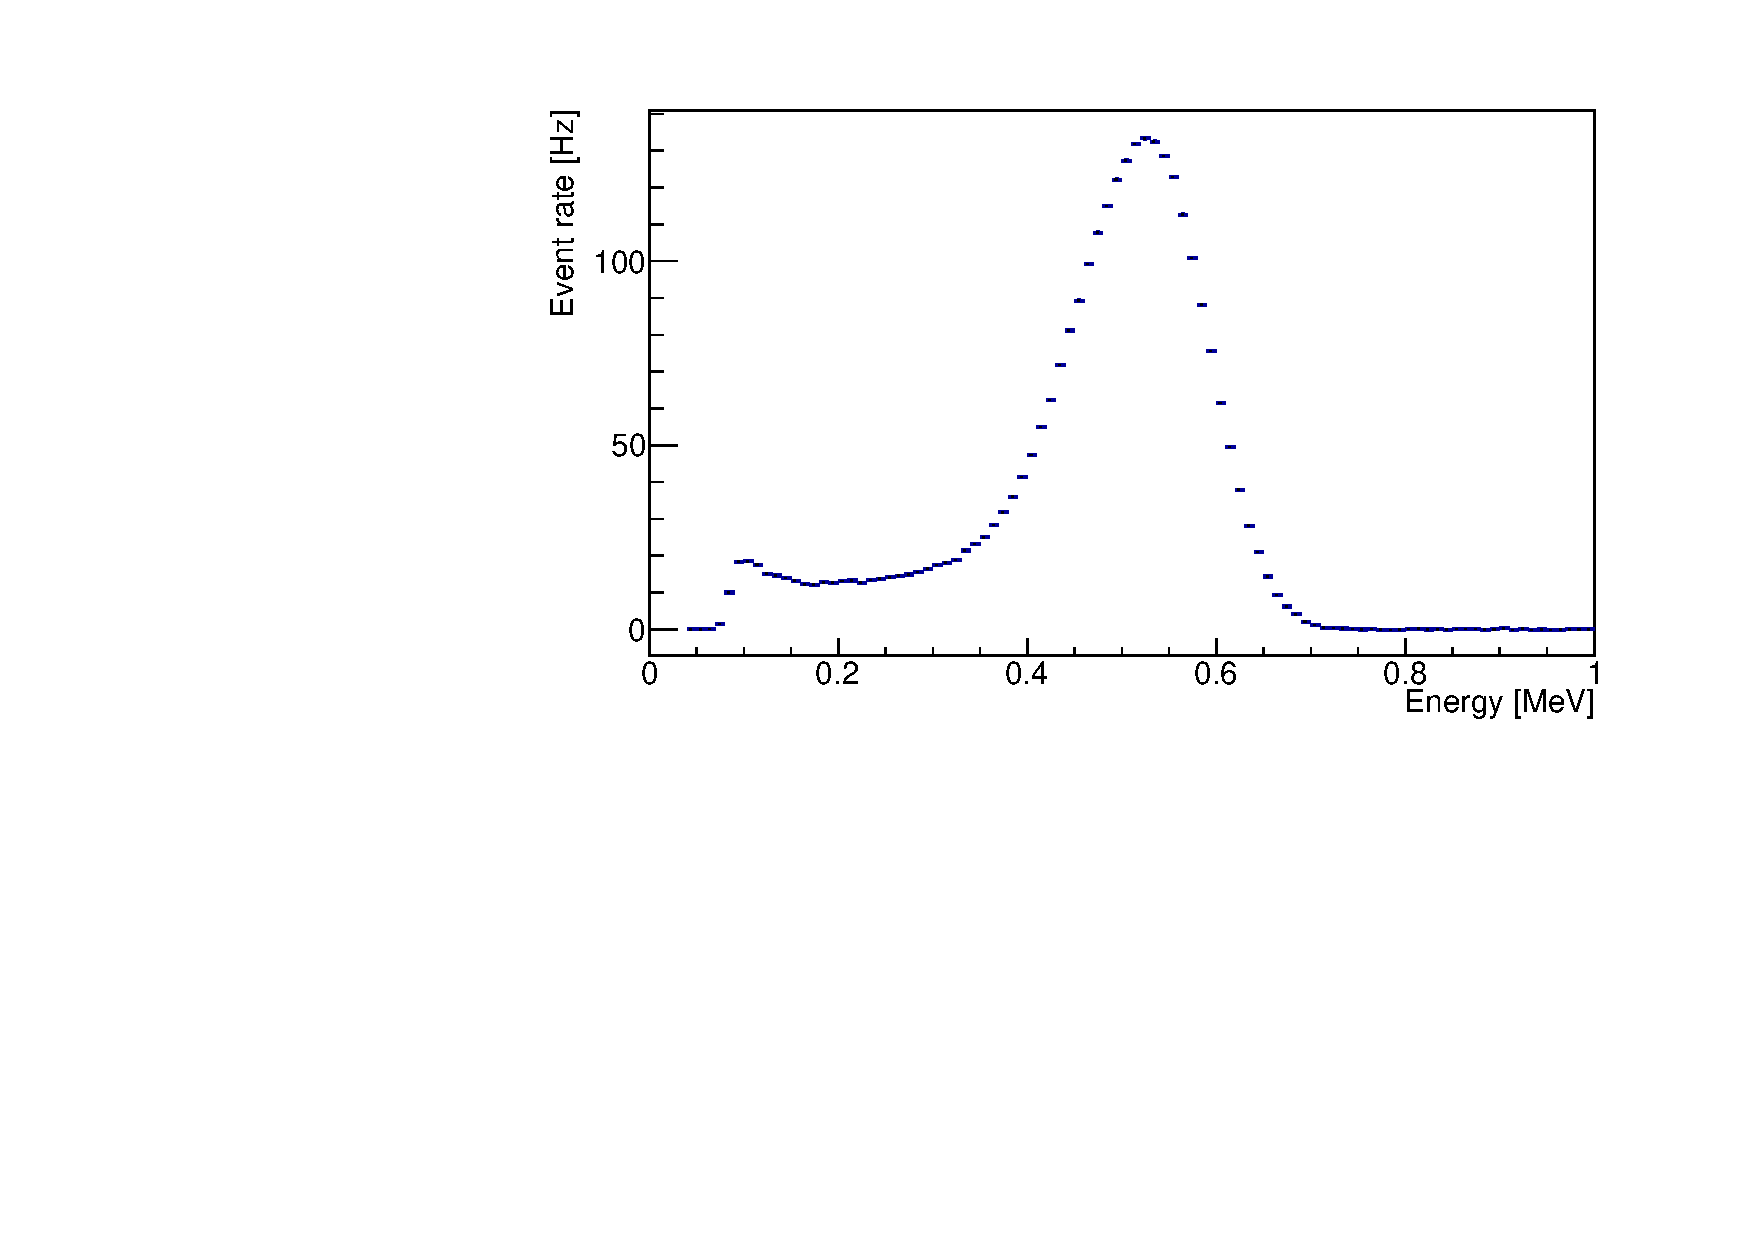
\includegraphics[width=60mm]{figures/Cs137smear85.pdf}}\quad
\subfigure[The gamma energy distribution from $^{22}$Na calibration.]{\label{fig:calibb}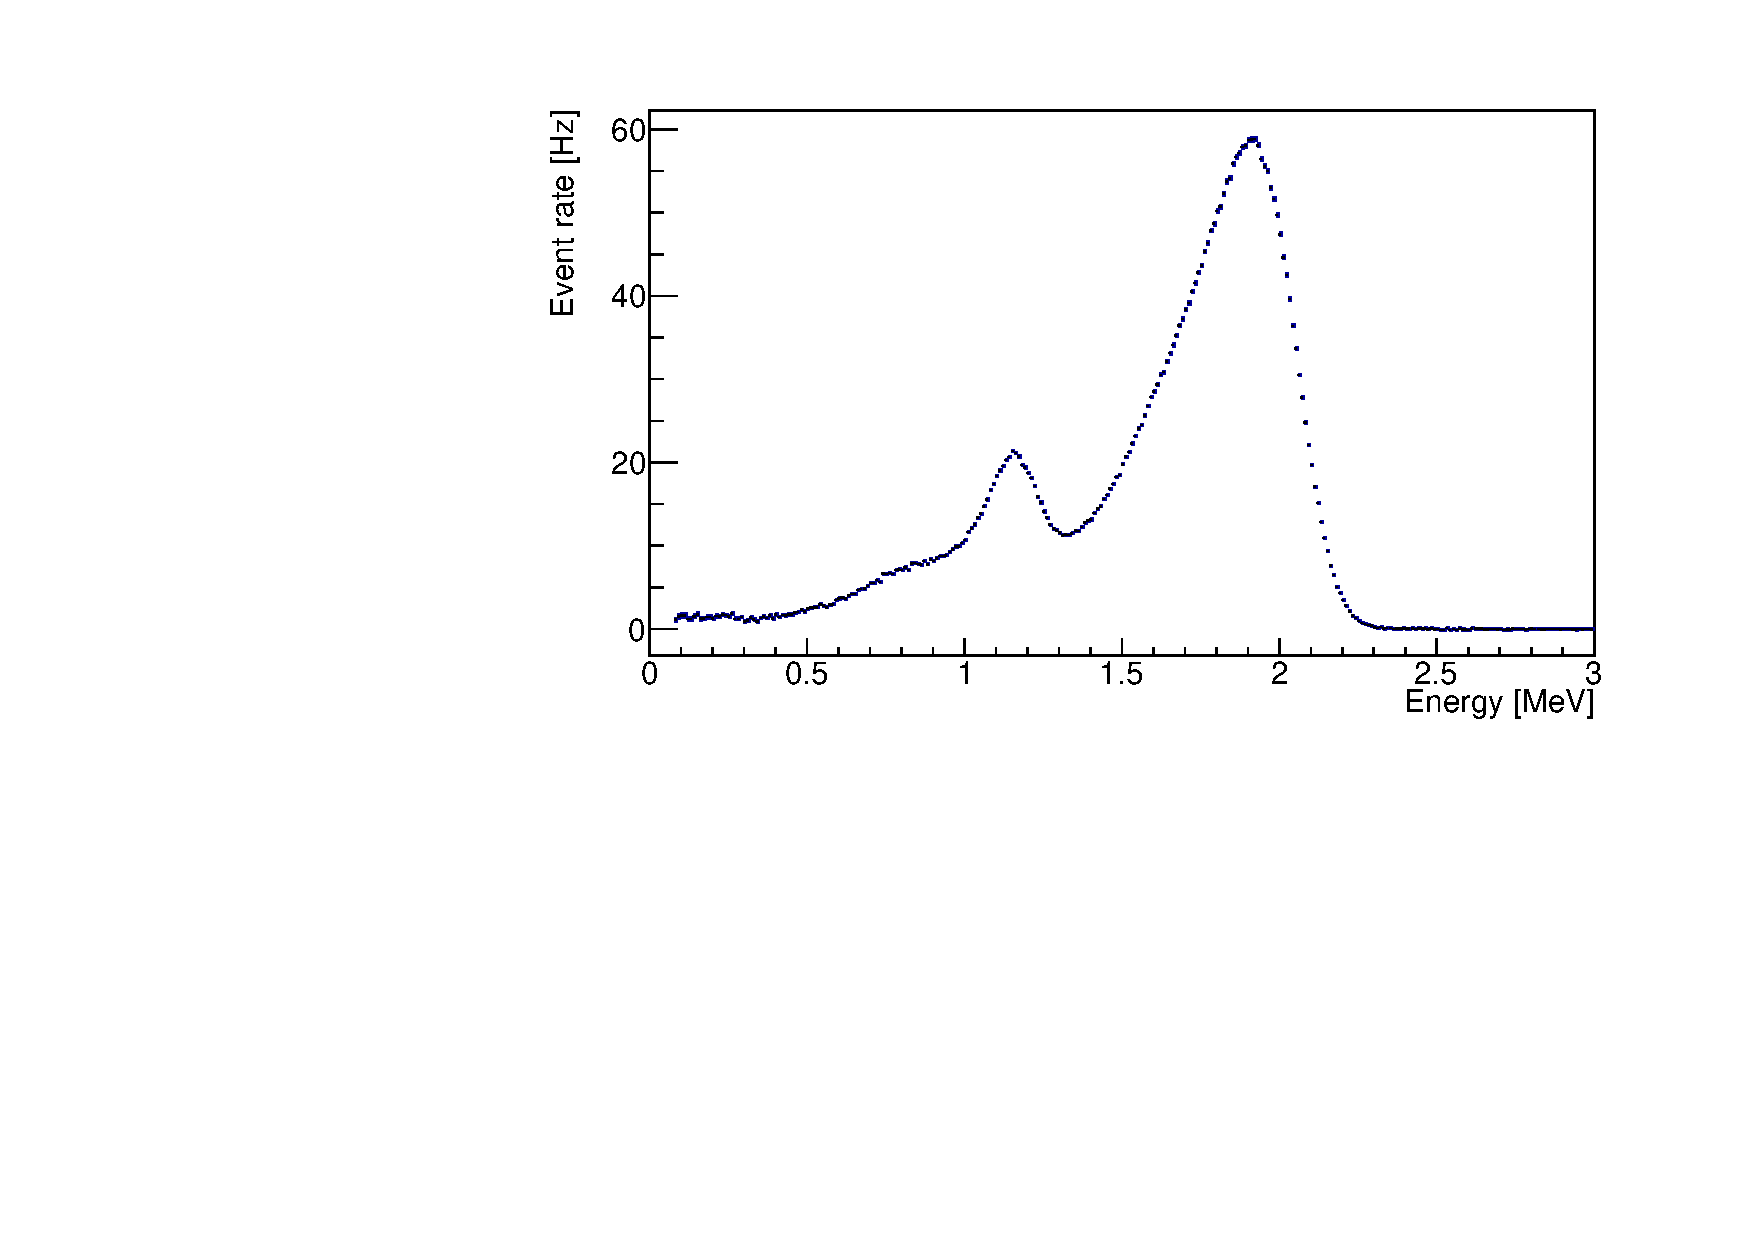
\includegraphics[width=60mm]{figures/Na22smear85.pdf}} \\
\subfigure[The gamma energy distribution from $^{60}$Co calibration.]{\label{fig:calibc}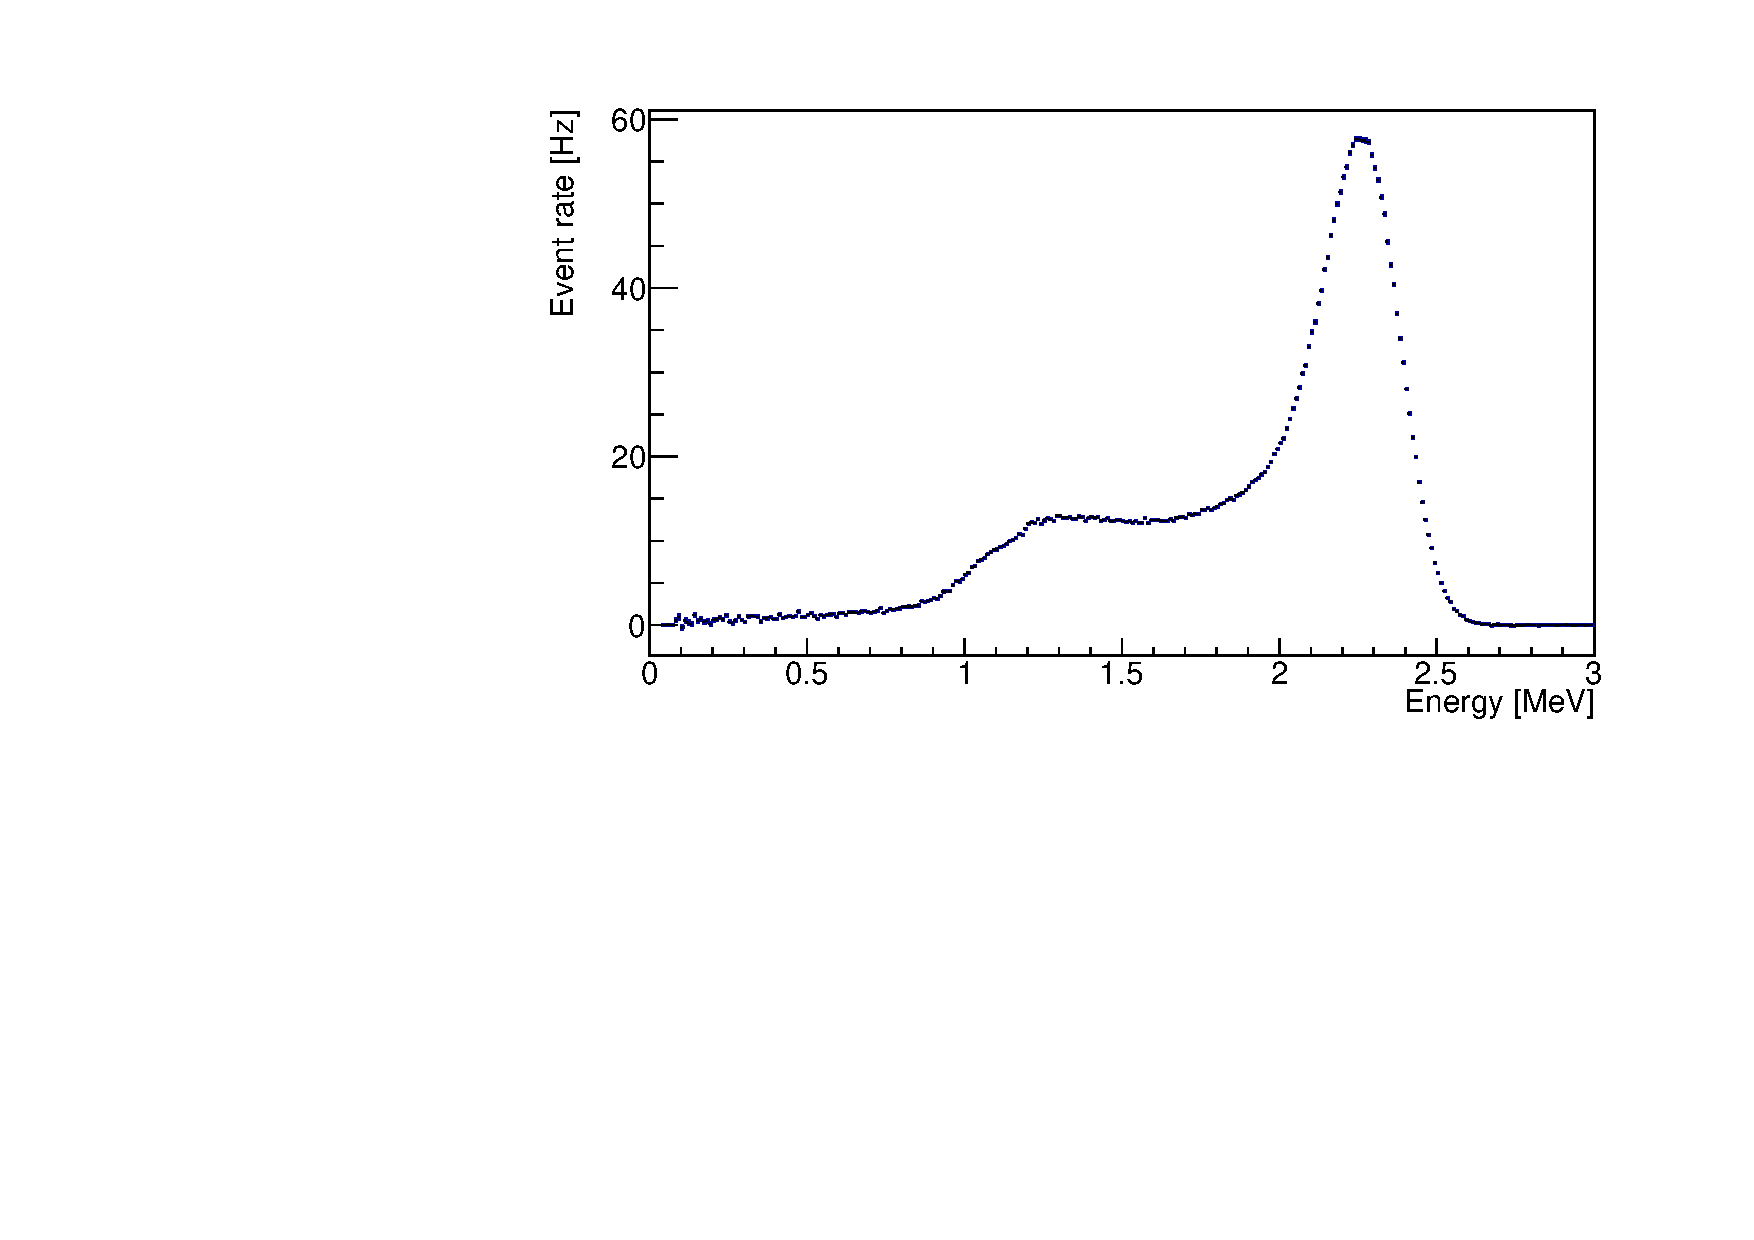
\includegraphics[width=60mm]{figures/Co60smear85.pdf}} 
\subfigure[The gamma energy distribution from neutron captured by hydrogen.]{\label{fig:calibd}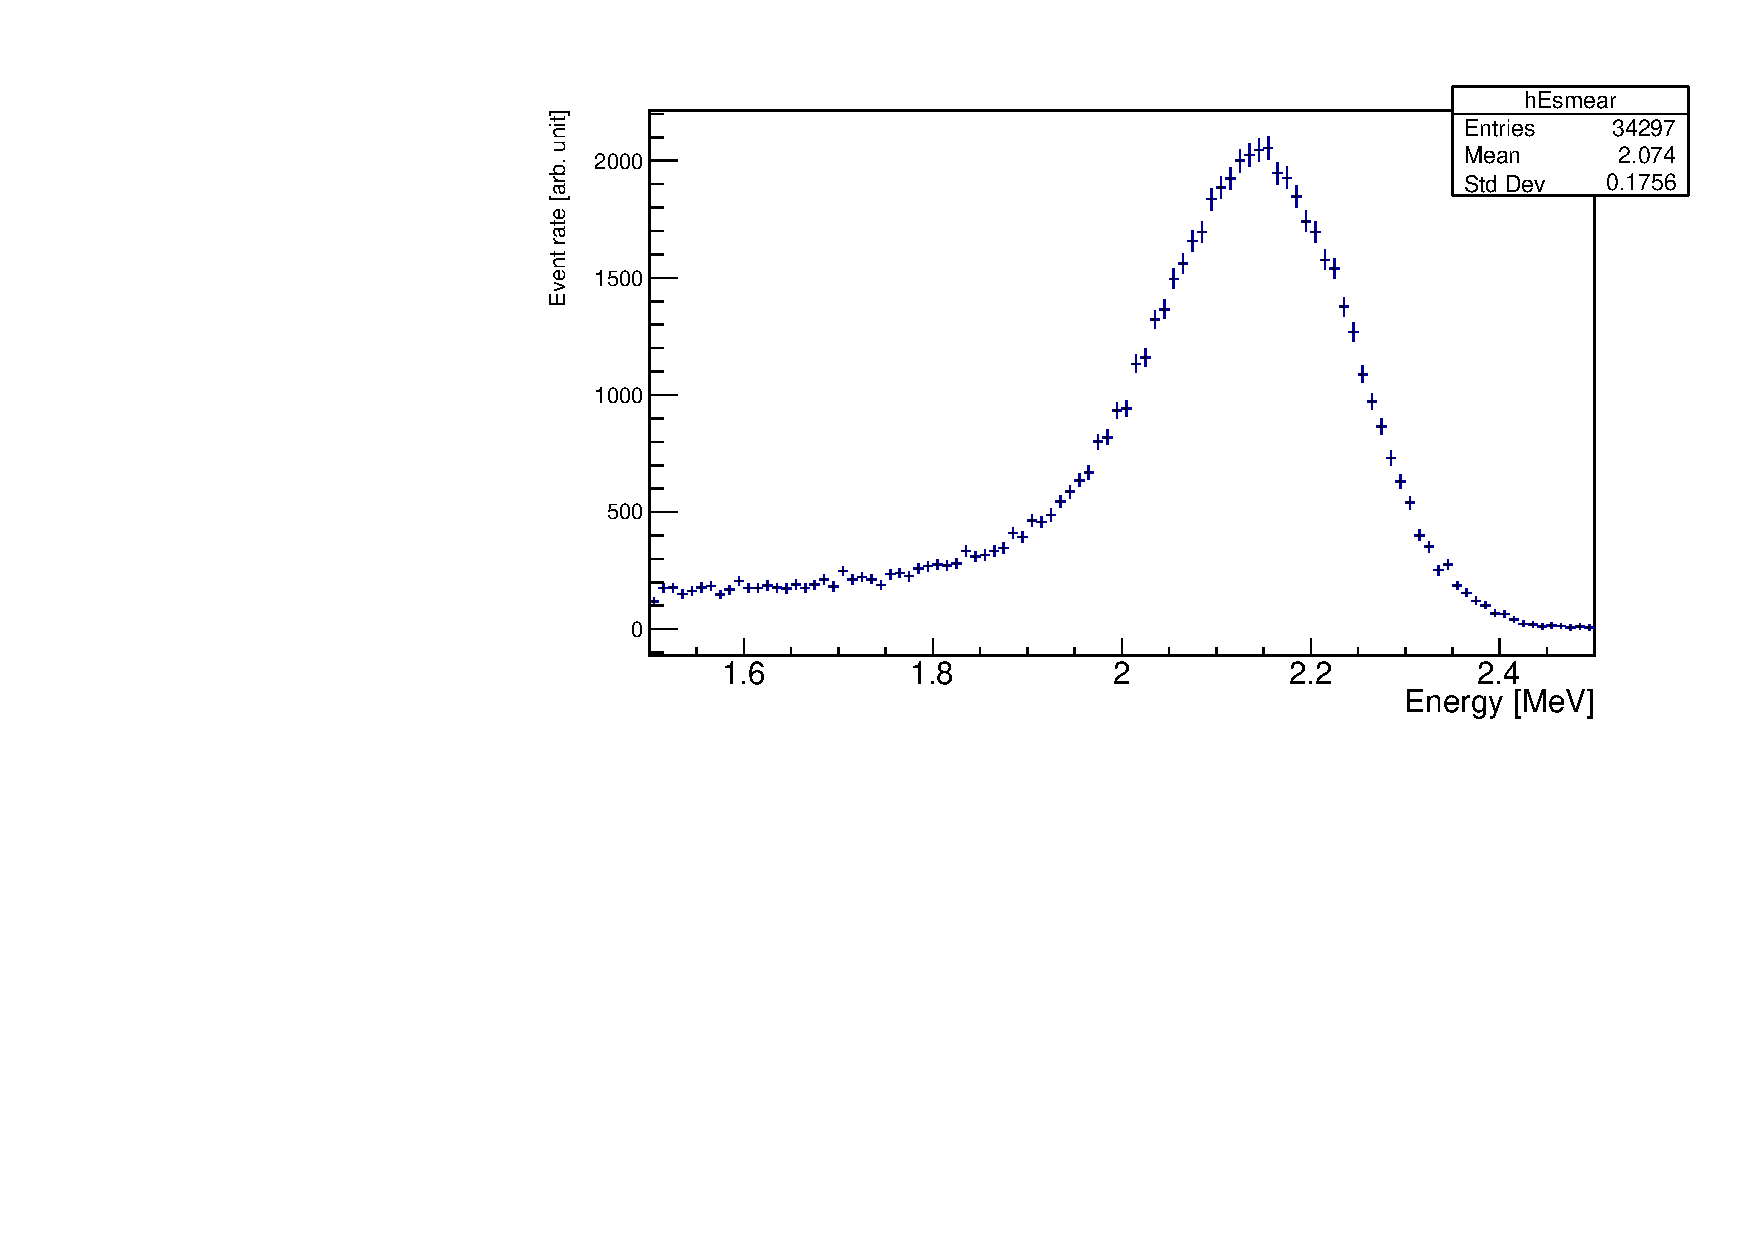
\includegraphics[width=60mm]{figures/Cf252smear85.pdf}}
\caption{The gamma spectra of calibration sources.}
\label{fig:gammacalib}
\end{figure}

The $^{12}$B is an ambient electron source in PROSPECT detector that is induced by cosmogenic neutron with $^{12}$C(n, p)$^{12}$B interaction.
The cross section of this interaction is $\sim 0.01$ barn. 
Because of its $\beta$ energy disttribution covers the higher enegy range of interest, it is a valuable calibration source to demonstrate the reconstructed energy scale of IBD events.
To acquire $^{12}$B events in PROSPECT, we collected recoil coincident ionization events by allowing the single-cell-hit recoil events in 0.7 to 10 MeVee range that followed by at most 3-cell-hit electron candidates with energy less than 20 MeV.
We required the delayed electron events to follow the single recoil event in 3 to 30 ms, while all electron events should be geometrically close to the recoil events and within the same fiducial volume of the IBD spectrum datasets.
In the procedure above, we used PSD to separate recoil and ionization events. The life time $^{12}$B decay was measured  $28.8\pm0.6$ ms that agreed with the norminal $29.14$ ms from ENSDF, shown in Figure \ref{fig:lifetime}. 
The prompt to delay distance is fitted with guassian distribution, the best fit stardard deviation = 2.91 cm, shown in Figure \ref{fig:distance}. 
During the 33 days of reactor off period, we collected about $\sim12000$ single-cell-hit $^{12}$B decay and $17514 <$3-cell-hits in full detector. 
The reconstructed spectrum of $^{12}$B electron is shown in \ref{fig:B12}.
\begin{figure}[h!]
\centering
\subfigure[The delay-prompt time difference of $^{12}$B candidates ]{\label{fig:lifetime}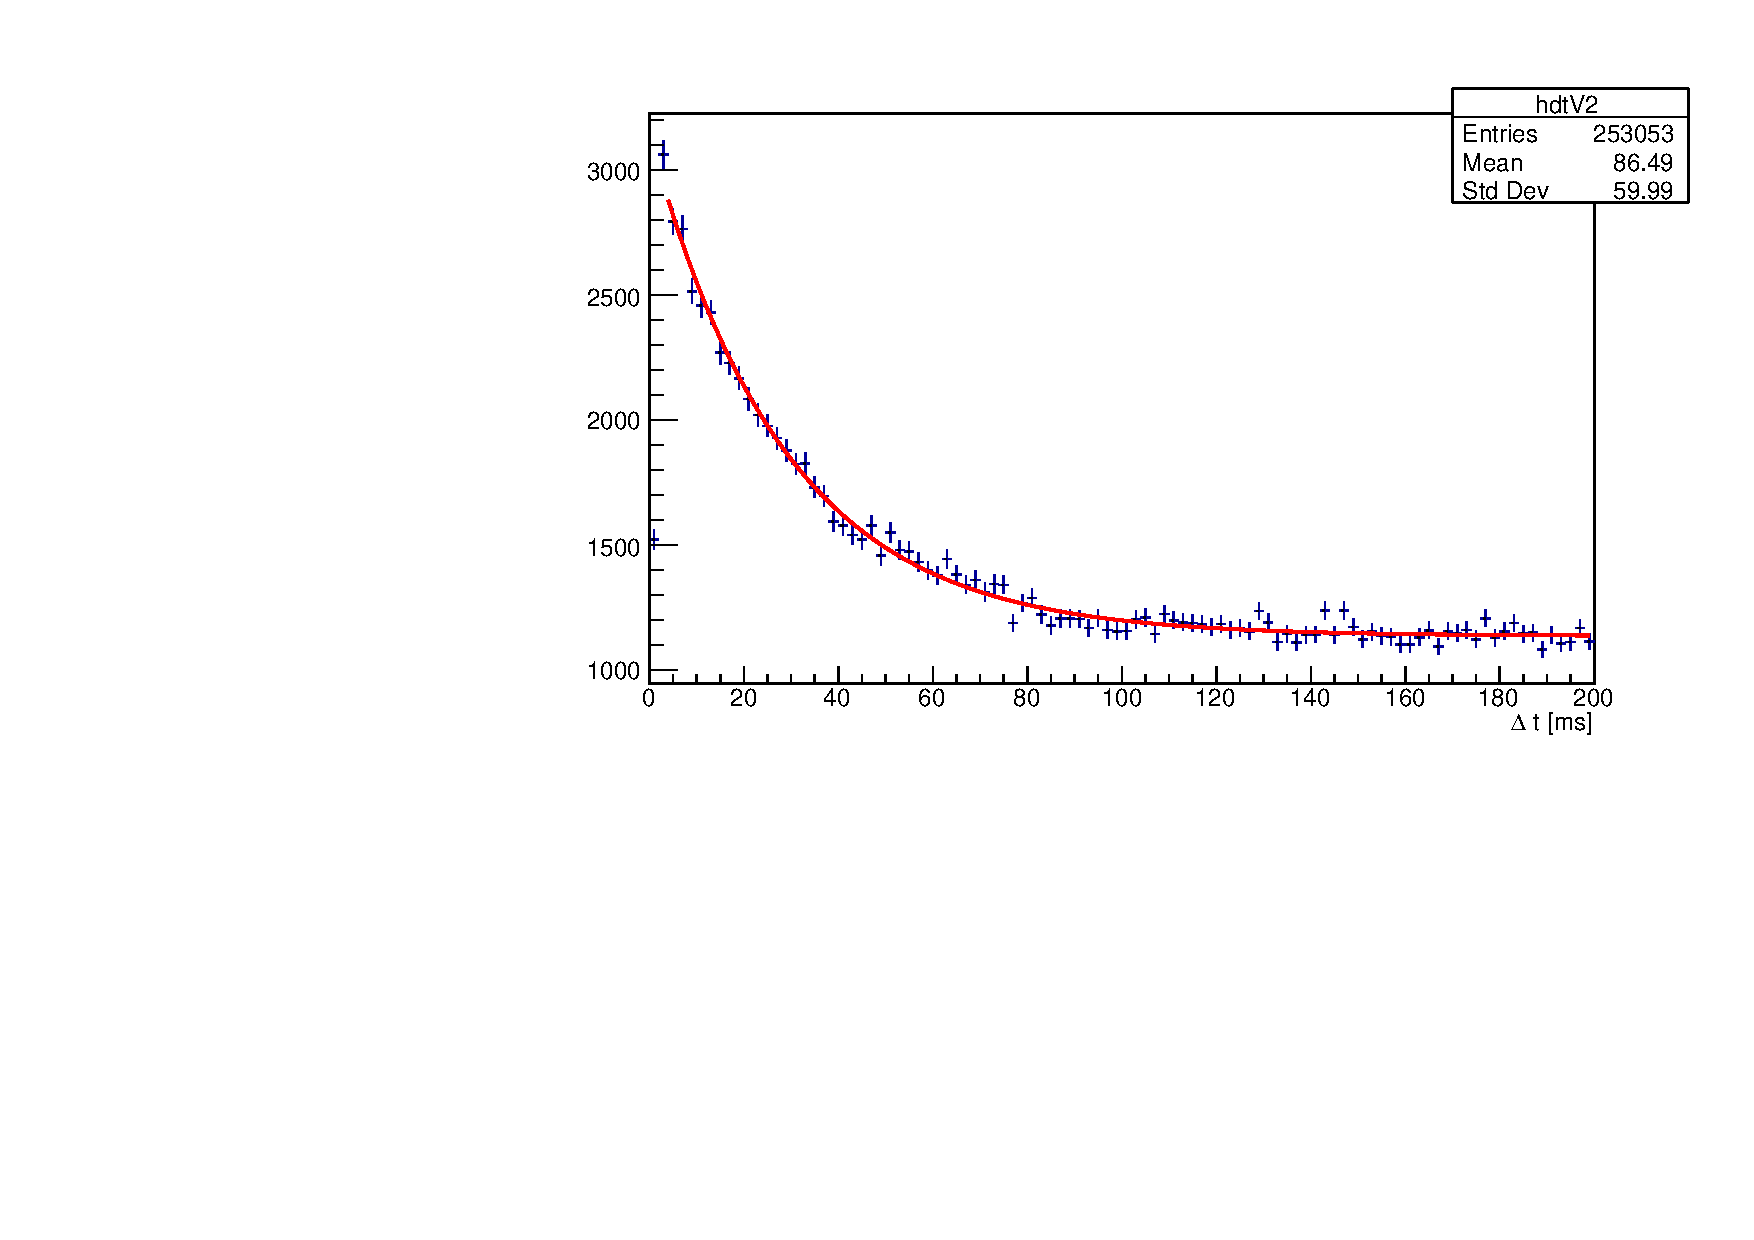
\includegraphics[width=60mm]{figures/B12dt85.pdf}}\quad
\subfigure[The delay-prompt distance of $^{12}$B candidates]{\label{fig:distance}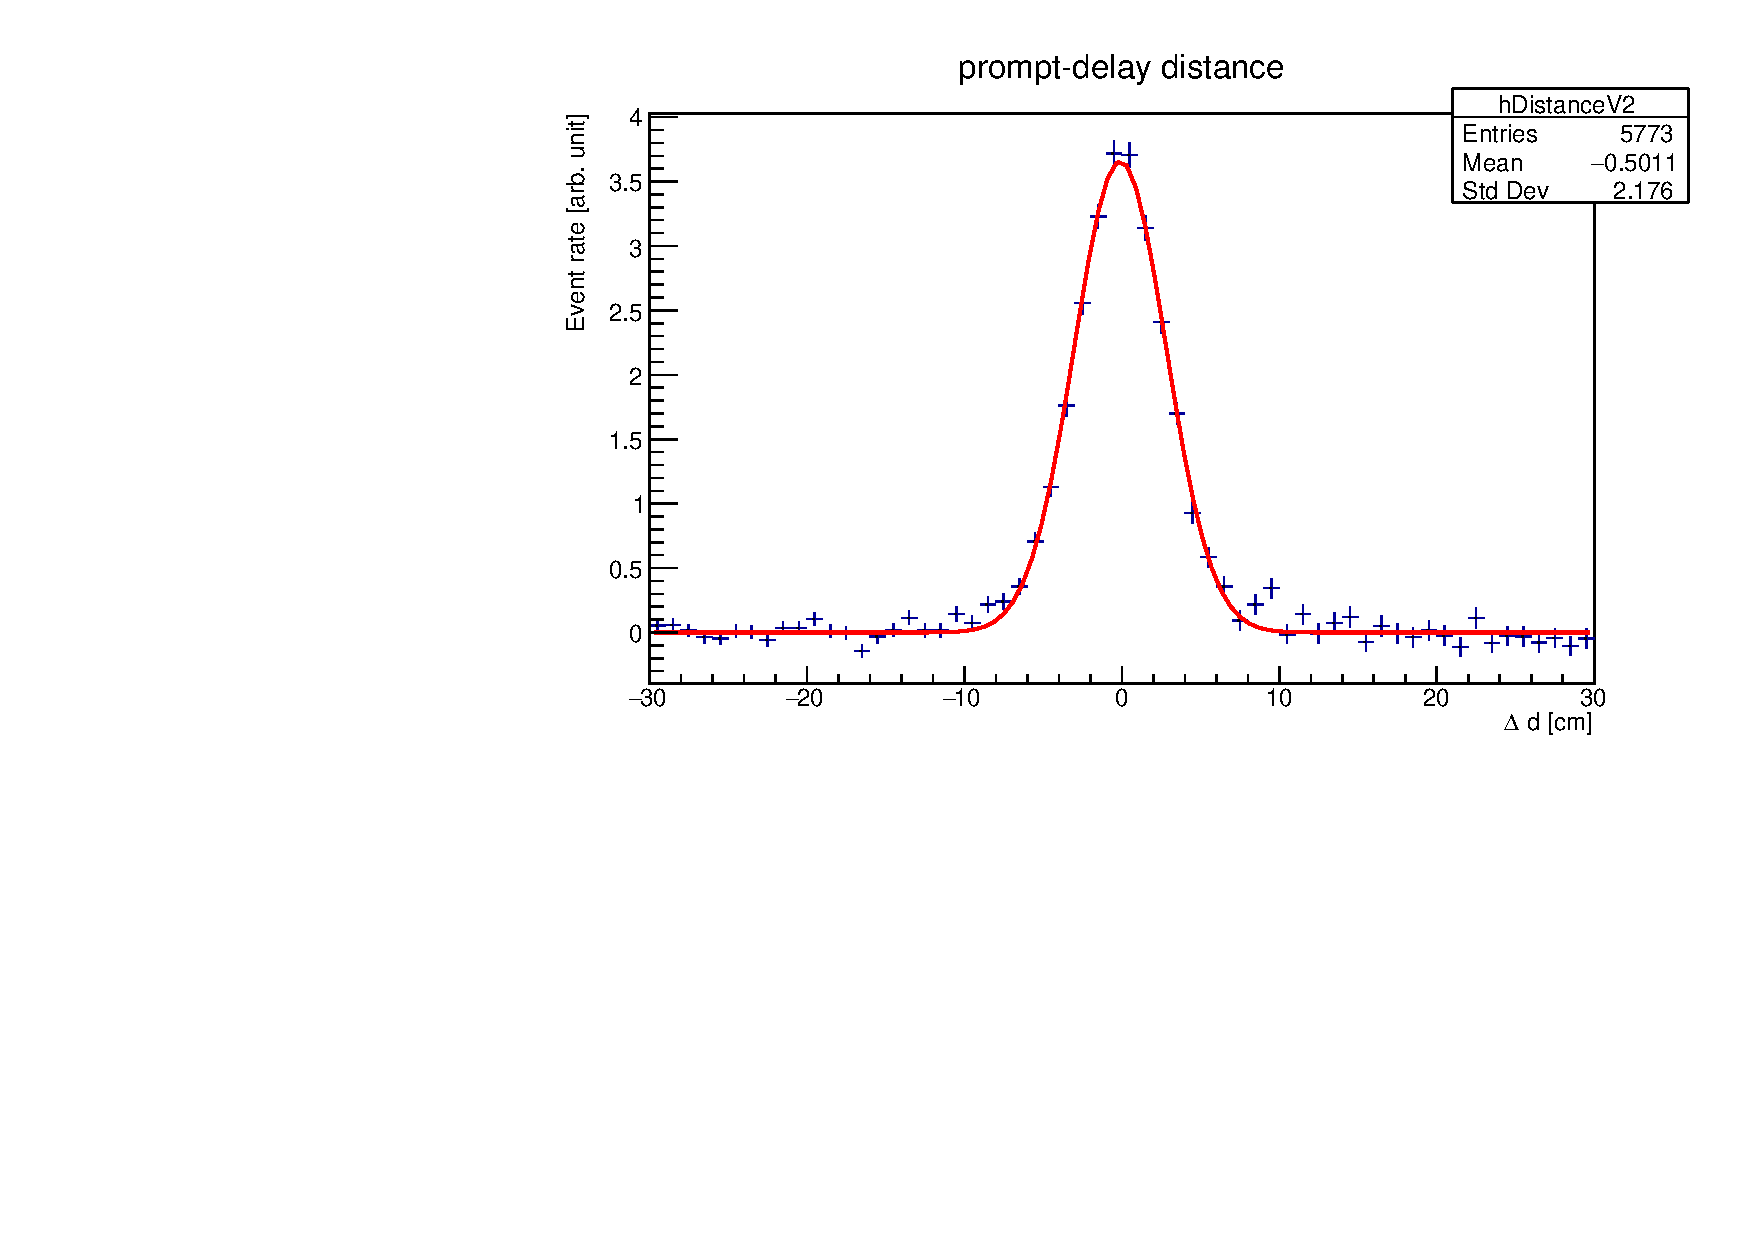
\includegraphics[width=60mm]{figures/B12distance85.pdf}} \\
\subfigure[$^{12}$B spectrum.]{\label{fig:B12}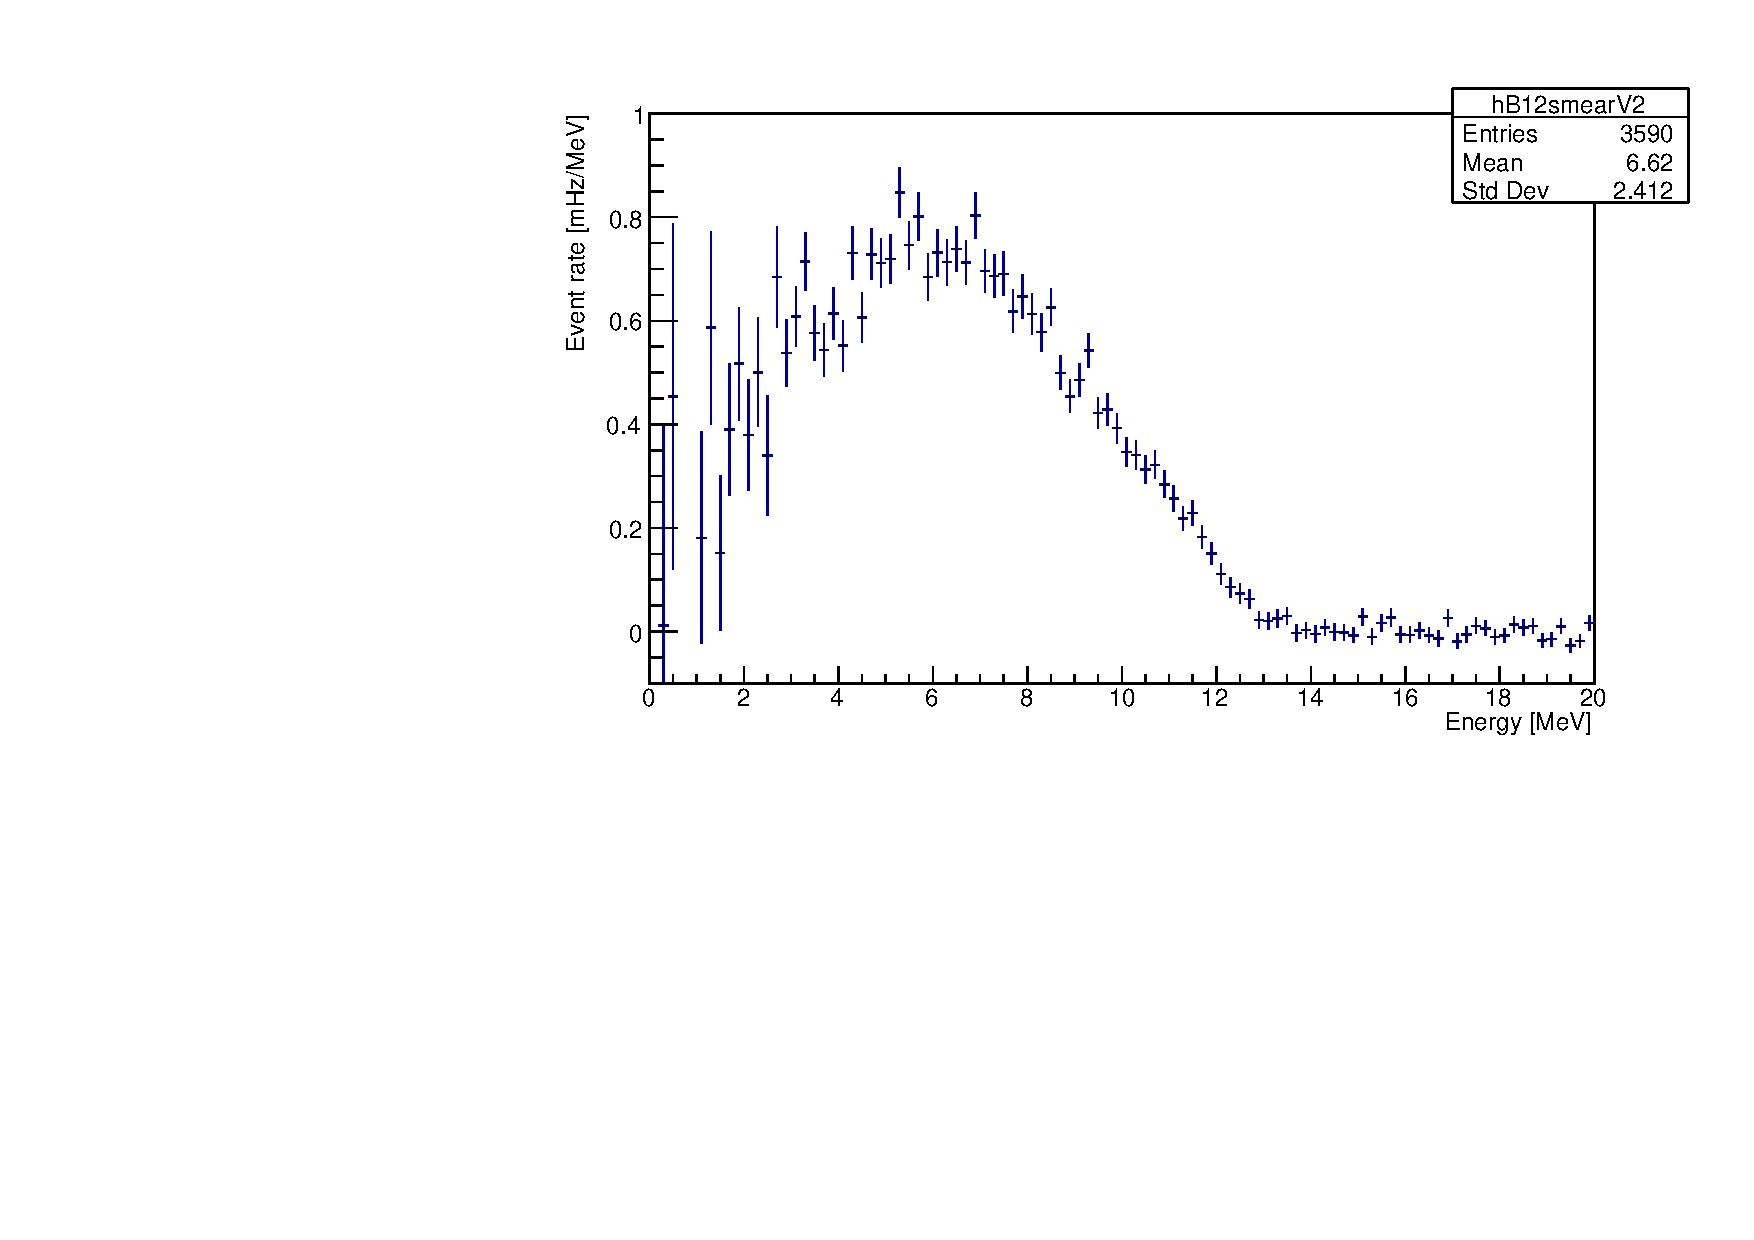
\includegraphics[width=60mm]{figures/B12smear85.pdf}} 
\caption{The observation of $^{12}$B events in PROSPECT.}
\label{fig:B12plots}
\end{figure}
\newpage

\clearpage

\section{Monte-Carlo Calibration Datasets}
The purpose of the comparison between Monte-Carlo and calibration data is to characterize the detector energy response, so we are able to provide trust worthy IBD prompt energy spectrum model with precisely tweaked detector response model.
The detector response includes the LS's photoelectric effect and detector geometry influence. 
The quenching effect, the optical properties of detector and the Cherenkov radiation induced by energetic particle can cause nonlinear energy reconstruction of incident event.
Meanwhile, detector geometry affects the reconstructed energy with gamma escaping and energy loss.
In addition, there are relative energy scale affected by the difference among detector cells, caused by possible nonuniformity of LS and cell volume.
The resolution of reconstructed energy are dominated by the time depent photostatistics of LS and the geometry effects of detector, but we had eliminate the fluctation of energy resoluton by uniformly smearing the energy of every hits.
The artificial smearing was based on the worst energy resolution (lowest PE/MeV) calibrated during the production data and through ou the detector.
As a result, the first and second order Birk’s constant in detector $k_{B1}$ and $k_{B2}$, the detect efficiency of Cherenkov light $k_{C}$, the absolute energy scale $\beta$ are the terms we needed to search precisely. 
Later in this study, we will review the energy resolution as function of energy based on the model with best-fit values of the parameters listed above.

The PROSPECT-G4 simulation package was utilized to simulate all of the calibration with close-to-reality detector configurations as calibration data.
Other than the detector geometry and materials, the nonlinearity from Birks$^\prime$ quenching effect of scintillator and Cherenkov radiation induced by charged particles was simulated by PROSPECT-G4.

\subsection{Nonlinearity}
\label{sec:nonlinear}
The energy response of LS is mainly affected by the Birks$^\prime$ law quenching and Cherenkov radiation. 

The Birks$^\prime$ law is a empirical function of the light yield per track length:
\begin{equation}
    \frac{dL}{dx} = \frac{\frac{dE}{dx}}{1+k_{B1}\frac{dE}{dx}+k_{B2}(\frac{dE}{dx})^2},
\end{equation}
where $k_{B1}$ are $k_{B2}$ the Birks$^\prime$ constants relate to property of LS. 
They represent the quenched reconstructed energy in LS, a nonlinear energy loss caused by particle-molecule interaction. 
According to the function, $k_{B1}$ reduces the reconstructed energy of lower energy events, showed in Figure \ref{fig:kb1plot}.
Although $k_{B2}$'s effect is negligible in higher energy, it is capable to affect event cell-hit multiplicity for its ability to quench more lower energy events below the 85 keV threshold, as shown in Figure \ref{fig:kb2plot}.
In MC, we  simulate the quenching effect by multiplying energy difference in between photoelectron steps with a Birk's factor:
\begin{equation}
   \frac{1}{1+k_{B1}\frac{dE}{dx}+k_{B2}(\frac{dE}{dx})^2}.
   \label{eql:birks}
\end{equation}

\begin{figure}[h!]
\centering
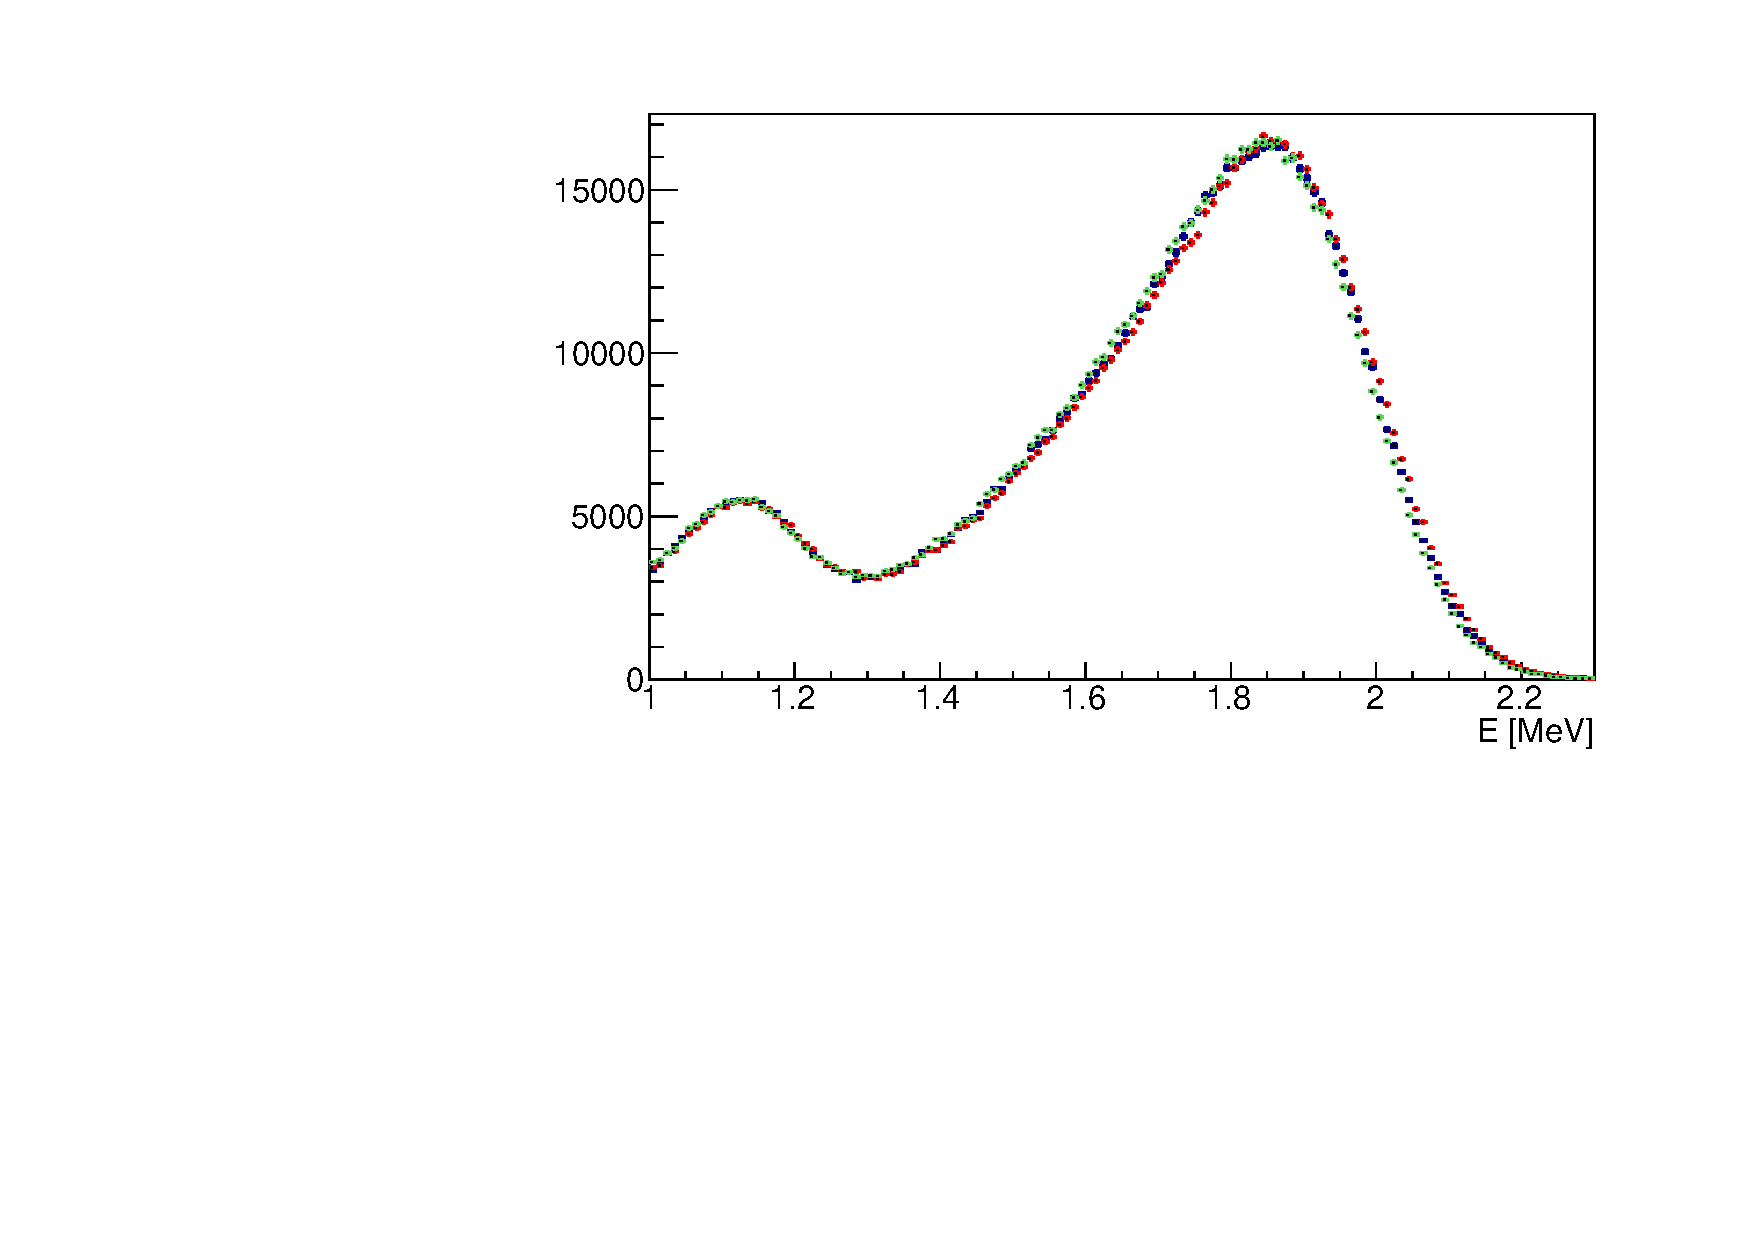
\includegraphics[width=60mm]{figures/kb1.pdf}
\caption{The MC quenching induced by $k_{B1}$. (red: lower value, blue: norminal value, green: higher value)}
\label{fig:kb1plot}
\end{figure}
 
\begin{figure}[h!]
\centering
\subfigure[The energy distribution of $^{22}$Na simulation affected by $k_{B2}$.]{\label{fig:kb2}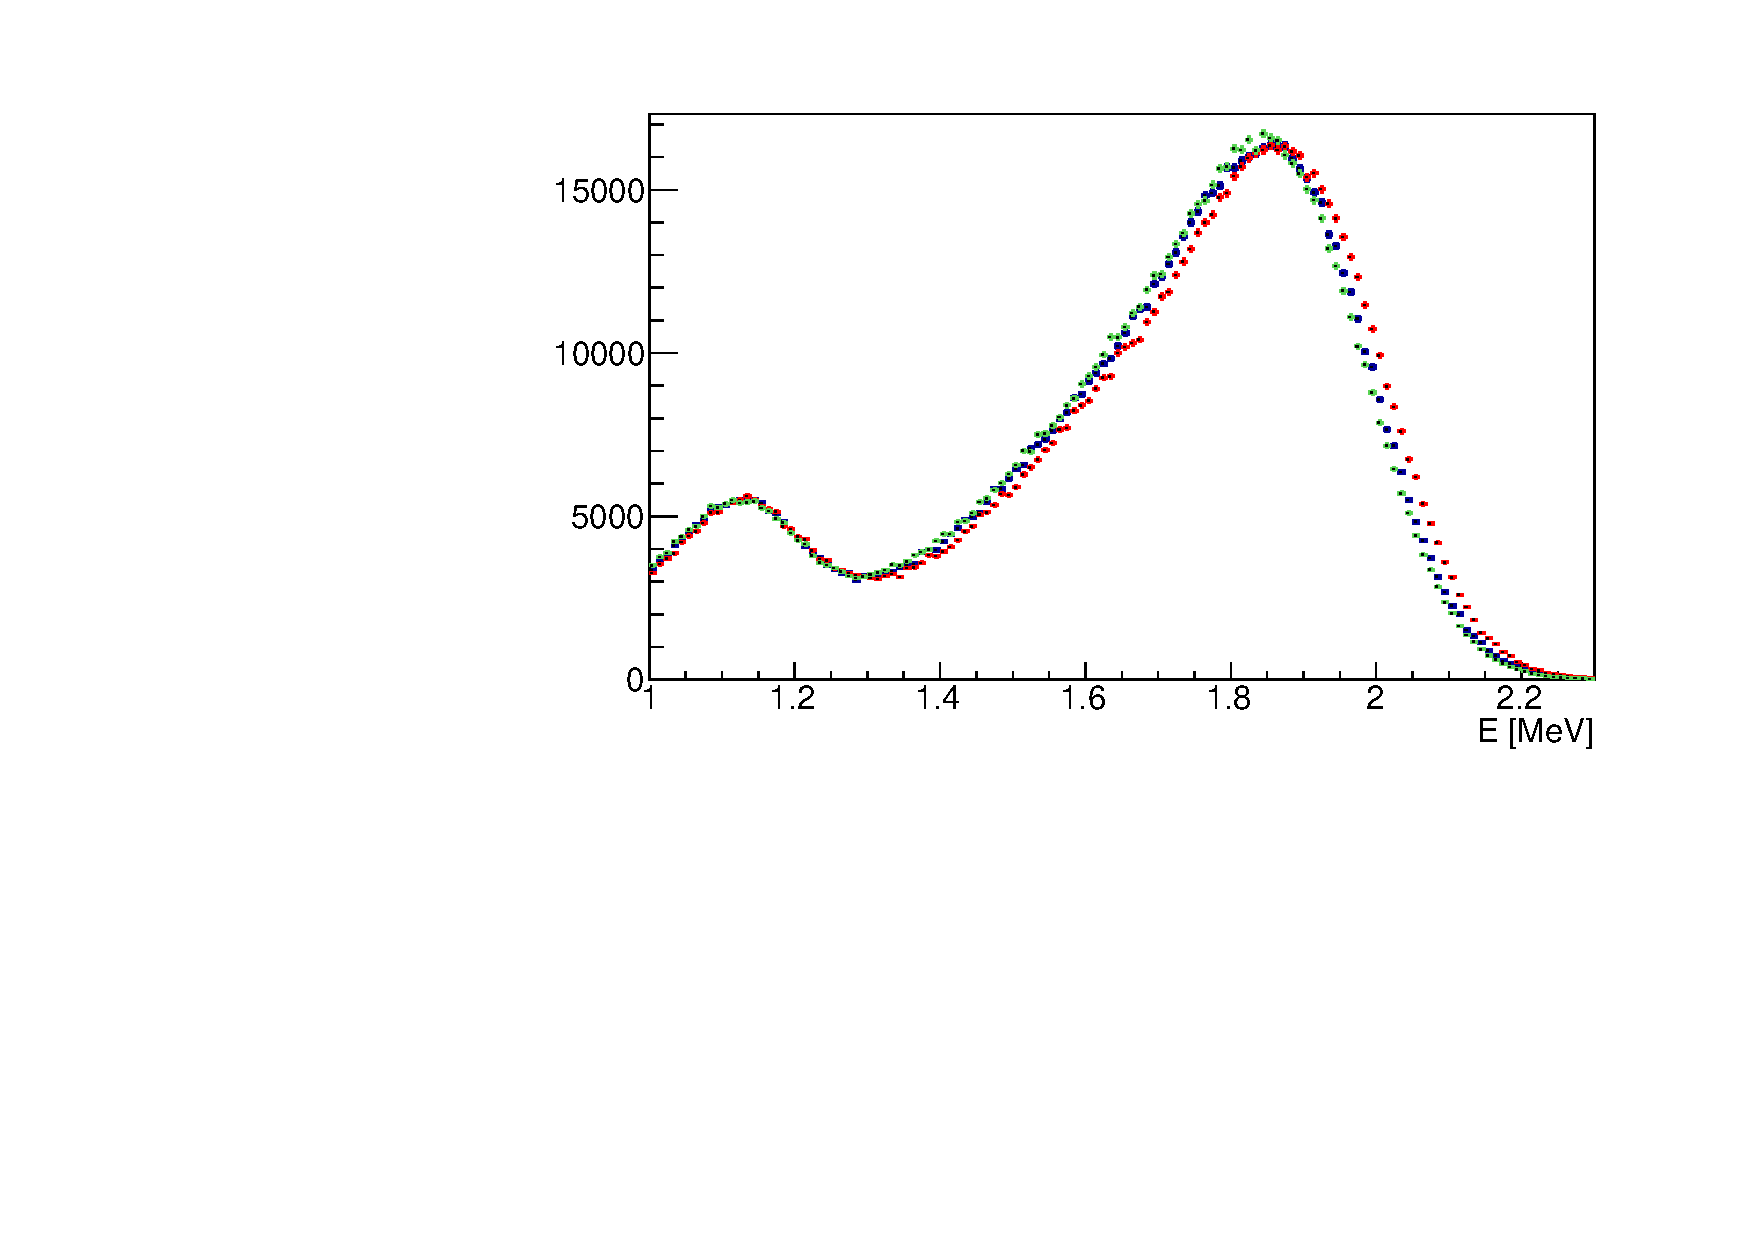
\includegraphics[width=60mm]{figures/kb2.pdf}}\quad
\subfigure[The $^{22}$Na cell-hit multiplicity affected by $k_{B2}$. ]{\label{fig:kb2multi}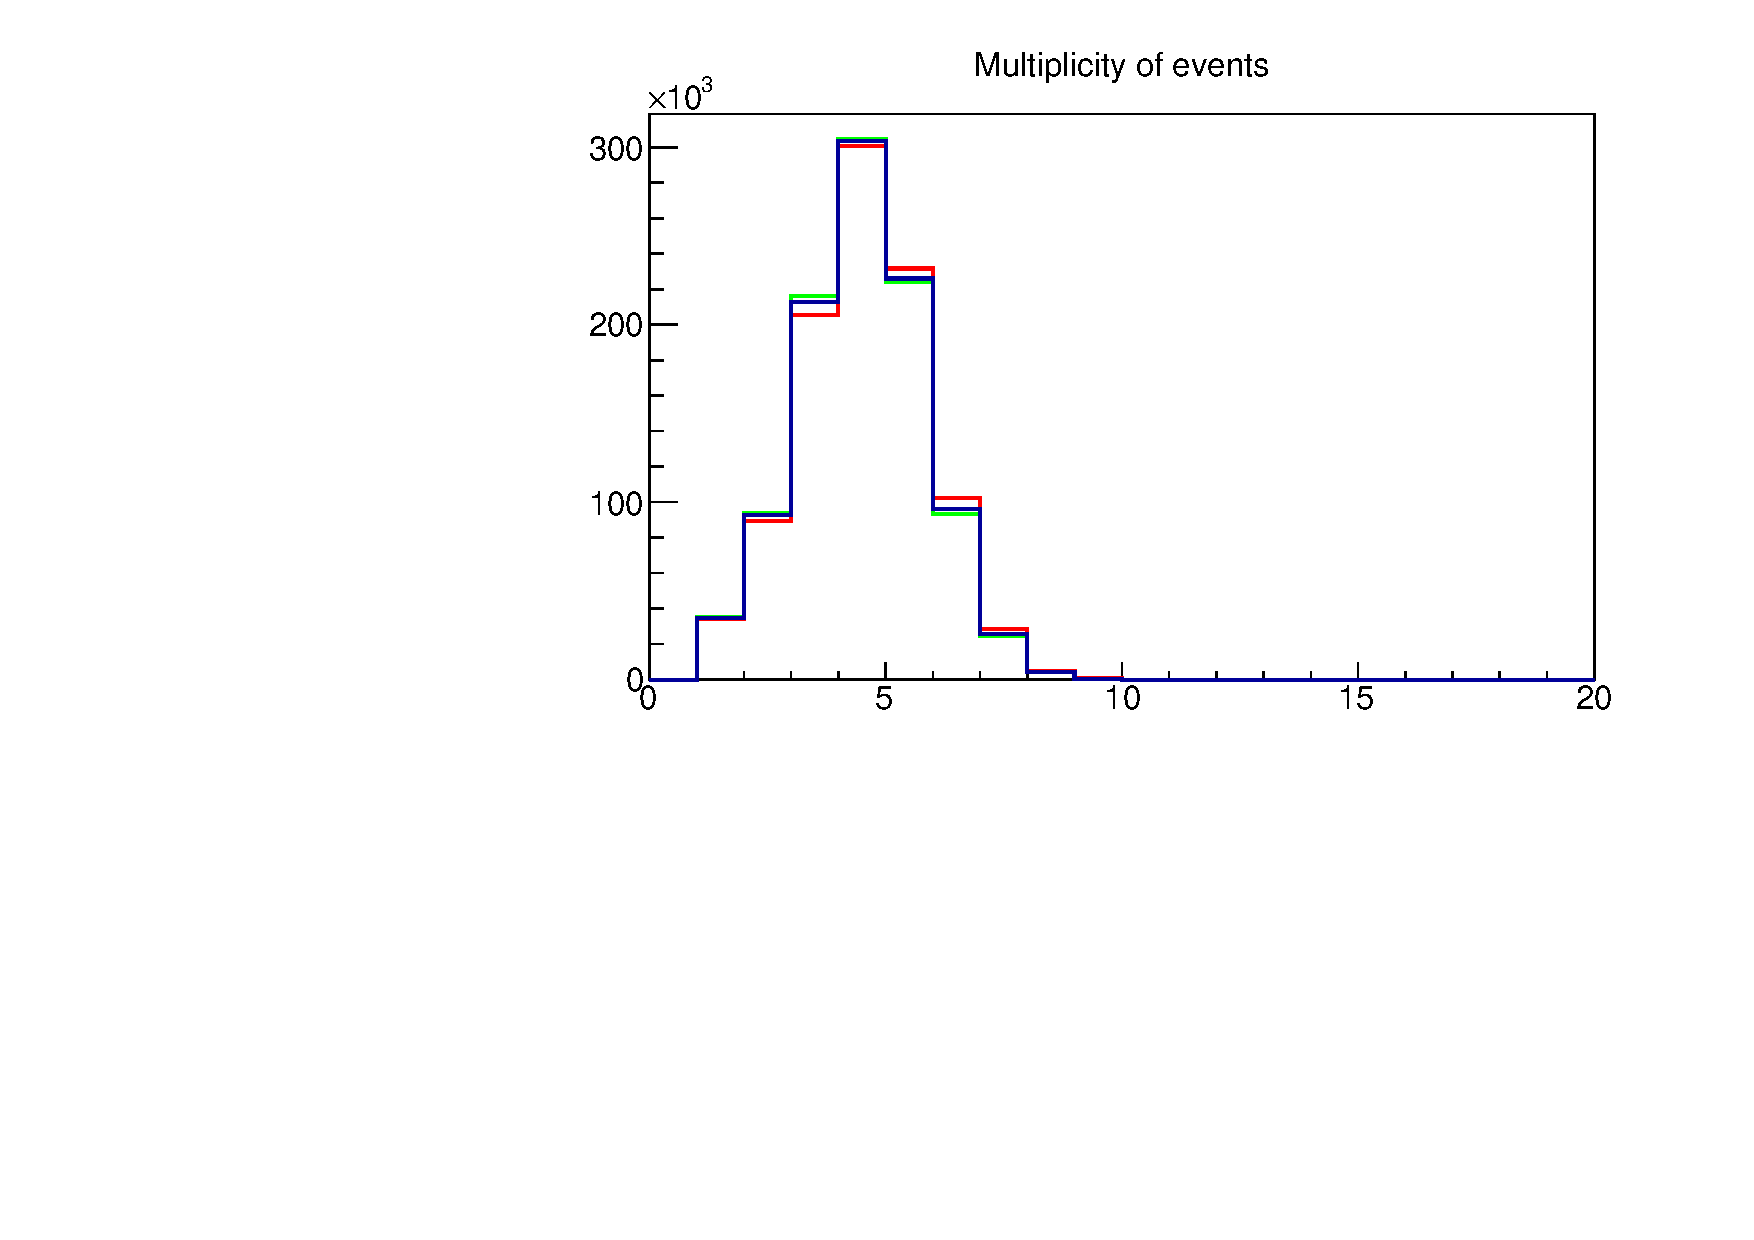
\includegraphics[width=60mm]{figures/kb2multi.pdf}}
\caption{The MC quenching induced by $k_{B2}$. (red: lower value, blue: norminal value, green: higher value)}
\label{fig:kb2plot}
\end{figure}

The Cherenkov radiation is the light emitted as a charged particle traveling faster than the phase velocity of light in a medium. 
The molecules in the medium are polarized along the particle track, when the particle is faster than light, the electromagnetic field of molecule depolarization can add up as coherent light emission. 
The number of photon generated along the particle track can be expressed as:
\begin{equation}
    \frac{d^2N}{dxd\lambda} = \frac{2\pi\alpha z^2}{\lambda}\left(1- \frac{1}{\beta^2n^2(\lambda)}\right),
\end{equation}
where $N$ is number of photon, $\alpha$ is a fine structure constant, $z$ is the particle's electric charge, $\beta$ is the speed of the particle and $n(\lambda)$ is index of refraction.
Although most of Cherenkov light is in UV range, the LS is able to absorb and re-emit it in VIS range with currently unknown efficiency.
Therefore, more light can be collected in addition to the scintillation light with high energy incident charged particle and increase reconstructed energy.
In MC processing, we collected the energy emitted from the Cherenkov radiation as the summed energy of detected Cherenkov photons. 
We also assumed the LS's index of refraction and detect efficiency remain same against wavelengths in 200-700 nm range.
Then we use the the detect efficiency of Cherenkov light, $k_{C}$, in percentage, to model the effect of Cherenkov radiation on reconstructed energy. 
The particle energy loss in Cherenkov radiation is negligible.
Figure \ref{fig:kcplot} showed different $k_{C}$ values affecting the n-H capture spectrum.

\begin{figure}[h!]
\centering
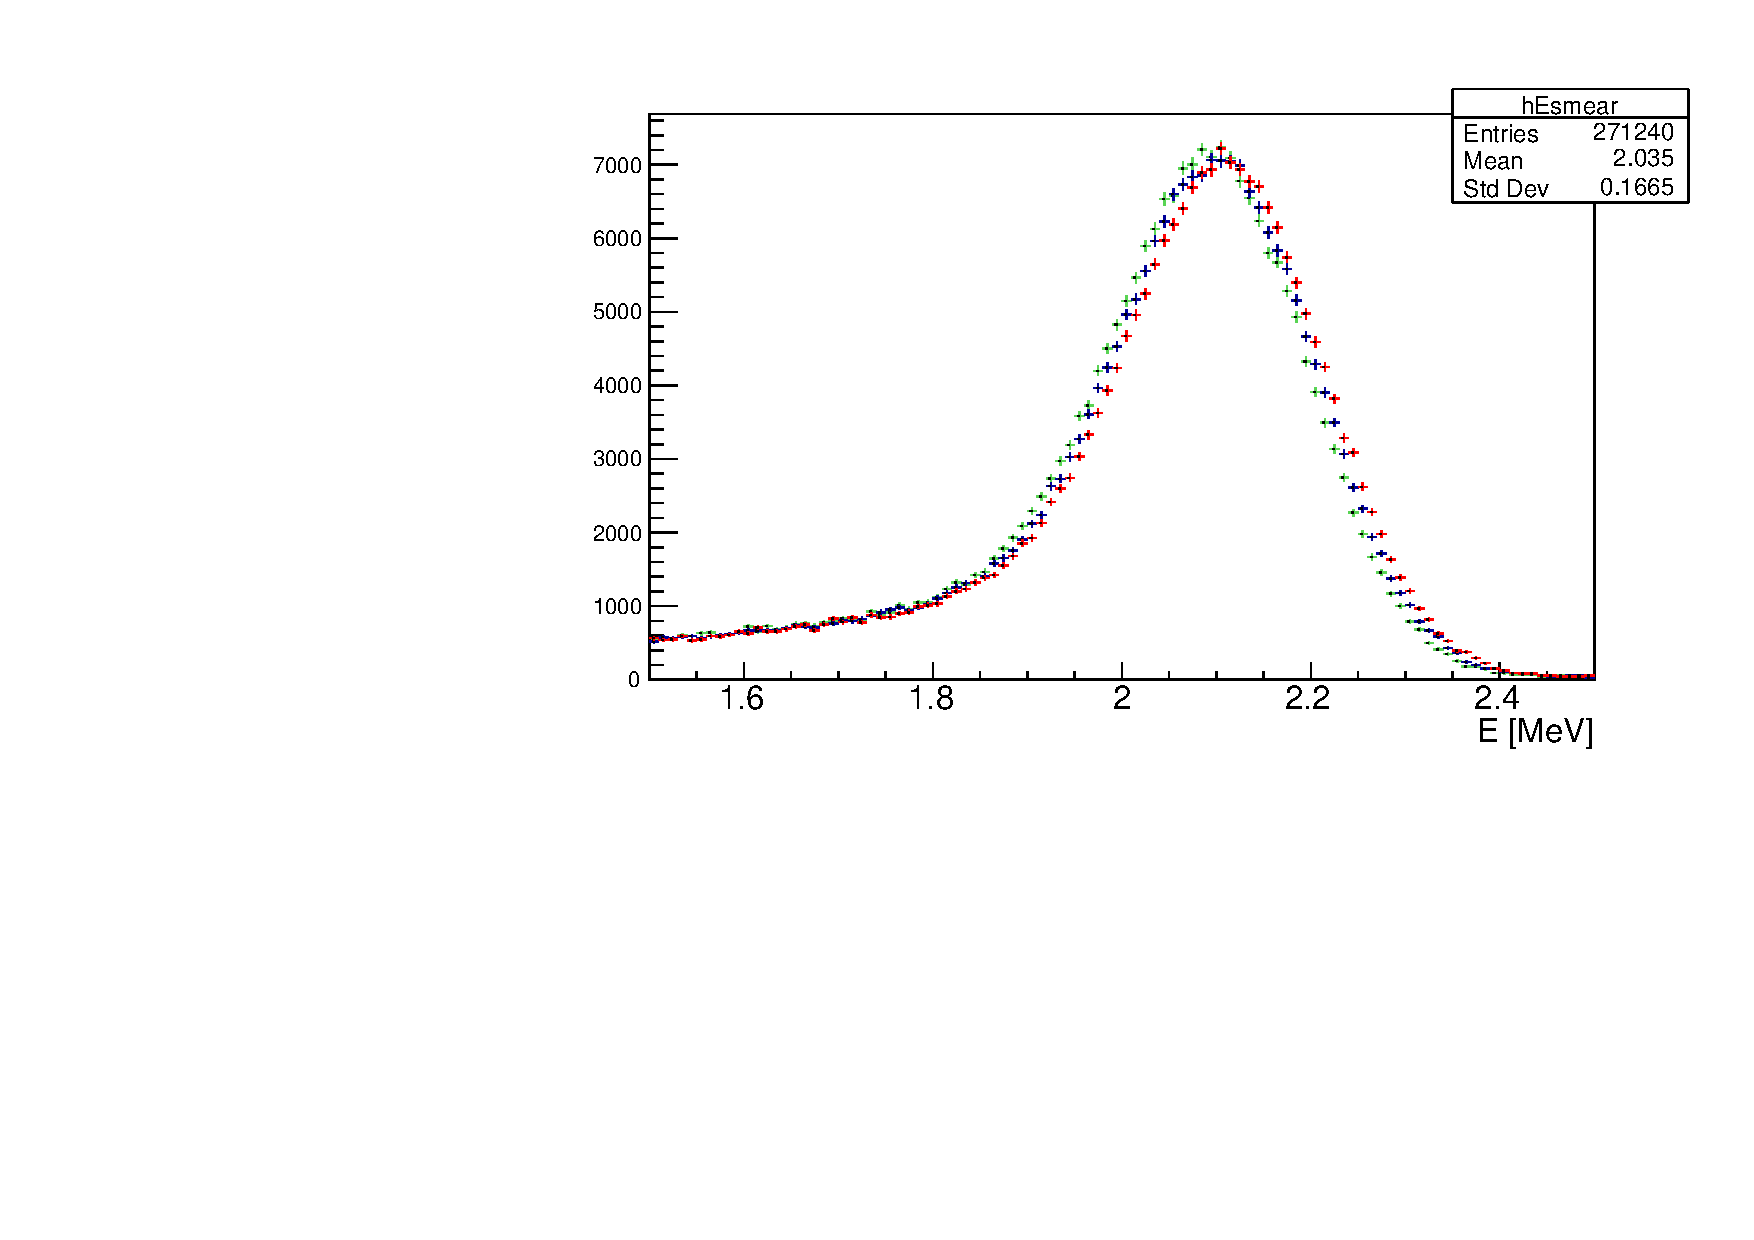
\includegraphics[width=60mm]{figures/kc.pdf}
\caption{The MC Cherenkov radiation effect induced by $k_{C}$. (green: lower $k_{C}$, blue: norminal $k_{C}$, red: higher $k_{C}$)}
\label{fig:kcplot}
\end{figure}

To simply model the detector energy scale, we adjusted the Birks$^\prime$ constants $k_{B1}$ and $k_{B2}$ in equation \ref{eql:birks} and the detect efficiency of Cherenkov light $k_C$ to search the best-fit nonlinearity model with data. The parameter search was in the range $(0.116, 0.136)$ mm/MeV for $k_{B1}$ with 0.002 mm/MeV steps, $(0.010, 0.030)$ mm/MeV for $k_{B2}$ with 0.002 mm/MeV steps and $(40, 50)\%$ for $k_C$ with $1\%$ steps. 
We performed calibration simulations for each group of the $k_B$s and $k_C$ combination and scanned through 1000 models .
The simulation involving optical photon is not realistic regarding to the scale of MC processed, we applied the nonlinearity corrections only to the energy of geant4 steps.

\subsection{Energy Resolution}
\label{sec:resolution}
The reconstructed resolution is a function of energy:
\begin{equation}
\label{eql:resolution}
    \frac{\sigma}{E} = \sqrt{a^2 + \frac{b^2}{E}+\frac{c^2}{E^2}},
\end{equation}
where $a$ is affected by the detector geometry, $b$ is from the photostatistics (PE/MeV) and $c$ for the quantum efficiency of PMTs.

%To reduce the computer resource required for the fitter, we neglected $a$ and $c$ of the resolution function, then used MINUIT $\chi^2$ minization to find the best $b$ value, while allow $b$ change freely.

\subsection{Other Energy Scale Factors}
\label{sec:other}
The reconstructed energy scale was initially based on the assumption that $n$ captured by $^6$Li yield 0.55 MeVee in detector. 
The deviation of true electron equivalent energy to this estimation can induce a constant energy scale throughout the all energy. 
This absolute energy scale $\beta_{rec}$, as a fitting parameter, was searched together with other energy response parameters.
Similar to the resolution term $b$, we allowed MINUIT minization of $\chi^2$ to freely change $\beta_{rec}$ until we found the minimum the $\chi^2$ between data and MC.

%The zero length encoding (ZLE) threshold was applied during data acquisition, requiring each ADC channel to record signals that are only above specific magnitude. 
%By excluding electronic noise, this threshold also affect the energy scale nonlinearly by excluding small deposition of energy in some segments in multi-hit events. 
To ensure MC being precisely compared to data, ZLE threshold was simulated in CalcDetectorPulseResponse program by convert energy deposit in MC to pulse with respect to ADC/PE ratio.
The 85 keV energy threshold was then applied to the calibration MC using same P2x analysis plugin.
%However, although quenching and detector effects were simulated in MC, the event selection based on the unsmeared energy of each hits (it is computationally expensive to smear simulation energy before energy cut, because it requires reanalyze MC everytime when each new resolution candidate is thrown).
%This reversed processing will result in MC keeping more low energy hits than data, then causing miss match between data and MC because of different cell-multiplicity per event.
%Thus a higher energy threshold whose smeared lower edge is close to the 85 keV is compromising.
%To resolve the issue with reversed data processing, an alternative energy threshold was searched from 65 to 90 keV with 5 keV steps.

\subsection{Detector Geometry Simulation}
The difference between simulated detector and the built detector could lead to disagreement in energy loss and gamma leakage between MC and data. 
The reconstructed energy of multi-cell-hit particle is affected by the separator thickness, pinwheel rod size and all materials that the particle can possibly travel through. 
In this work, we surveyed the thickness and material of the separator, the pinwheel rod dimensions and thickness, the inner structure inside pinwheel rods, the density and mixture of LS and calibration capsule properties, based on detector design and QA measurements.
Out of those detector properties, the thickness of separators play non-negligible roles in eventenergy loss. 
The thickness and uncertainty of the separator is $1.18 \pm 0.05$ mm, which is described in reference \cite{docThick}.

\begin{figure}[h!]
\centering
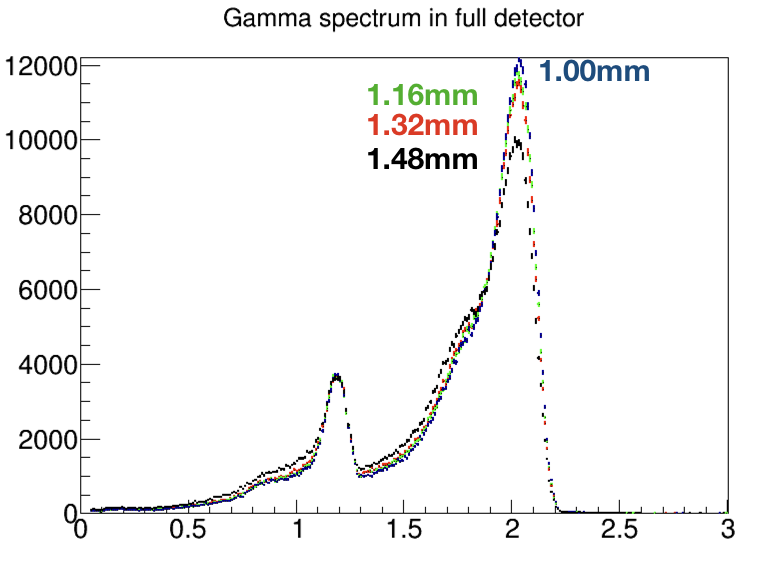
\includegraphics[width=80mm]{figures/thickness.png}
\caption{The example showing the thickness of separators affecting the energy loss and so the spectrum.}
\label{fig:thickness}
\end{figure}

Besides, we found the uncertainties of the dimensions of the other inner detector materials played negligible role in energy loss. 
For instance, the variation thickness of the pinwheel rode, which carries the similar uncertainty as separators, did not change the reconstructed energy visibly, even with exaggerated $0.25$ mm uncertainty showed in Figure \ref{fig:pinwheelthick}.

\begin{figure}[h!]
\centering
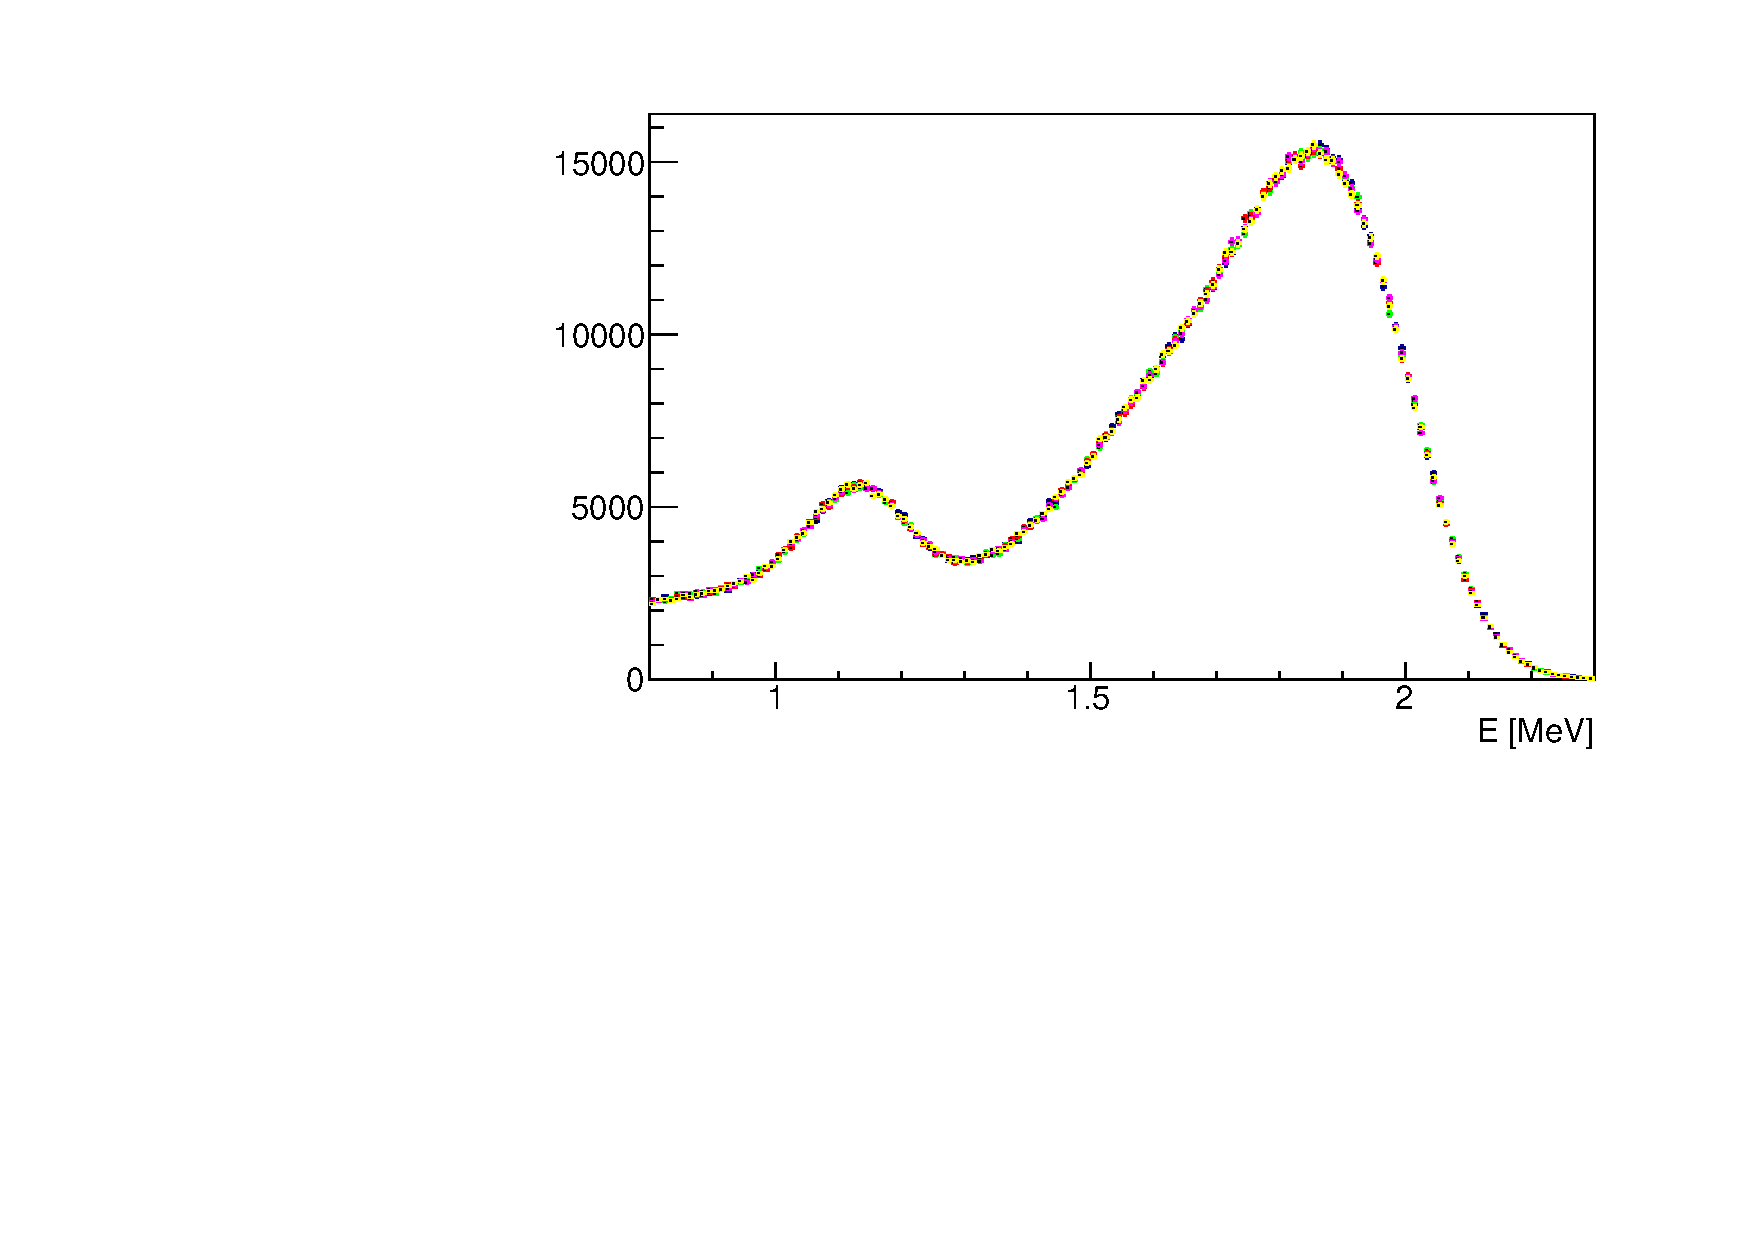
\includegraphics[width=80mm]{figures/pinwheelthick.pdf}
\caption{The example showing the thickness of piwheel rods$^\prime$ ignorable effect on the energy loss. (blue: 12.1 mm; red: 12.2 mm; green: 12.3 mm; pink: 12.4 mm; yellow: 12.5 mm)}
\label{fig:pinwheelthick}
\end{figure}

\subsection{Calibration Input Model}
The input model of radioactive calibrations was based on the decay branching from ENSDF database.
We simulated 1 million decays individually for each nonlinearity model scanned and each of the radioactive calibrations, which is comparible to the real event rates.
The decay branching fraction and energy scale in the simulation input are negligible.
The decay branches of $^{12}$B is based on reference \cite{duke}. 
We generated 250,000 $^{12}$B decays in simulation, which is considerably more stastics than data collected.
During data vs MC comparison, the $\sim$1\% energy scale uncertainty of $^{12}$B input spectrum was taken into consideration by pulling the energy scale of $^{12}$B spectrum in 1\%. 
The uncertainty in $^{12}$B decay branching fractions are negligible.

\section{Data vs Monte-Carlo Comparison}
\label{sec:dataMC}
The MC calibration spectra was compared with data through $\chi^2$ test. 
We generated a list of calibration MC with a variety of $k_B$ and $k_C$ as mensioned in section \ref{sec:nonlinear}. 
The MC file were converted to pulses and processed through similar analyzing loop as calibration data, except for smearing and thresholding order, as described.
The data vs. MC comparison was made with similar detector configuration, including same dead channels, comparible event rate and same fiducial volumes.
Then the analyzed MC spectra were scaled with a constant energy scale $\beta_{rec}$, while both data and MC were artificially smeared with the energy resolution as described in section \ref{sec:resolution}.
The MINUIT $\chi^2$ minimization method was utilized to find the best fit four parameters. 

We performed the $\chi^2$ minimization on data-MC comparison of full-detector reconstructed energy spectra.
The best-fit model was than demostrated by the cross-checking with the measured the single cells that are most adjacent to the gamma calibration sources.

\subsection{Full Detector Spectrum Comparison}
\label{sec:fulldet}
The full detector reconstructed energy spectrum is the distribution of the summed energy of every hit within an event cluster. 
Each cluster is a group of hits collected by adjacent individual LS cells and the gap between each hit being less than 20 ns.
The detector nonlinearity affected the full detector energy spectrum not only through energy scale, but also through cell-hit multiplicity, for different quenching coefficient can reserve or reject hits through the 85 keV threshold of single cell measured energy.
Therefore, in our searching of the best-fit nonlinearity model, we aimed to minimized the $\chi^2$ of a combined data-MC energy spectrum and hit multilicity comparison. 
In detail, the data-MC comparisons of the energy spectrum of gamma calibrations, the n-H capture gamma from $^{252}$Cf and $\beta$-decay of $^{12}$B were done simultaneously.
Considering the precision of event source location, we performed multiplicity comparison only on the gamma calibrations, containing $^{22}$Na, $^{137}$Cs and $^{60}$Co.

%As discussed in section \ref{sec:single}, the full detector reconstructed energy was not only quenched by LS, but also affected by energy loss and particle leakeage caused by inner materials of detector.
%Besides, the energy threshold in each cell contributed to the energy loss indirectly by affecting the cell-multiplicity of events.
%Ideally, the full detector's quenching model is same as single cell and PG4 package is able to simulate these energy loss and thresholding effects. 
%However, currently the best fit parameters from full detector data vs MC comparison shows poor agreement with single-cell best fit.
%The most likely reason is an unresolved nonlinearity based on detector cell-multiplicity of the incident event, which is currently under investigation, but do not effect overall energy scale significantly.
%Given this context, we chose to examine two methods related to full-detector energy scales: applying BF single-cell parameters to full-detector data/MC comparison, and separately performing a minimization on the full-detector data/MC comparison.

%As mentioned in Section \ref{sec:other}, we scanned through a variety of threshold and found 85 keV threshold is able to effectively reproduce the cell-multiplicity events from data, whose lower energy bound after smearing converted to $\sim73$ keV by assuming energy resolution as $4.2\%/\sqrt{E}$.

In full detector data vs. MC comparison, for the radioactive source calibrations, we tagged the peaks of the energy spectrum and picked the $3-\sigma$ region around the peaks as range of fitting. 
For $^{12}$B comparison, we chose 3 to 13.5 MeV as energy range of interest.

The figure \ref{fig:goodfit2} shows the full detector calibration spectra comparison best-fit model, where $\chi^2/NDF = 807.847/331$ with the parameters: $k_{B1} = 0.122 \pm 0.002$ mm/MeV, $k_{B2} = 0.023 \pm 0.002$ mm/MeV $k_C = 41 \pm 1\%$, with absolute energy scale of $\beta_{rec} = 100.36\pm0.2\%$. 
There was $\chi^2/NDF = 205.9/60$ contributed by the multiplicity fitting.
In the energy spectra comparison, the biggest contributor of the disagreement is n-H capture gamma with $\chi^2/NDF = 175/40$.
The data-MC energy spectra comparison of the best-fit model is shown in Figure \ref{fig:goodfit2}, and multiplicity comparison is shonw in Figure \ref{fig:multi}.
The $\chi^2$ distributions depent on $k_{B1}$ and $k_{B2}$, and $k_{B1}$ and $k_{C}$ are shown in Figure \ref{fig:chi2}.

\begin{figure}[h!]
\centering
\subfigure[Full detector MC-data for $^{137}$Cs calibration.]{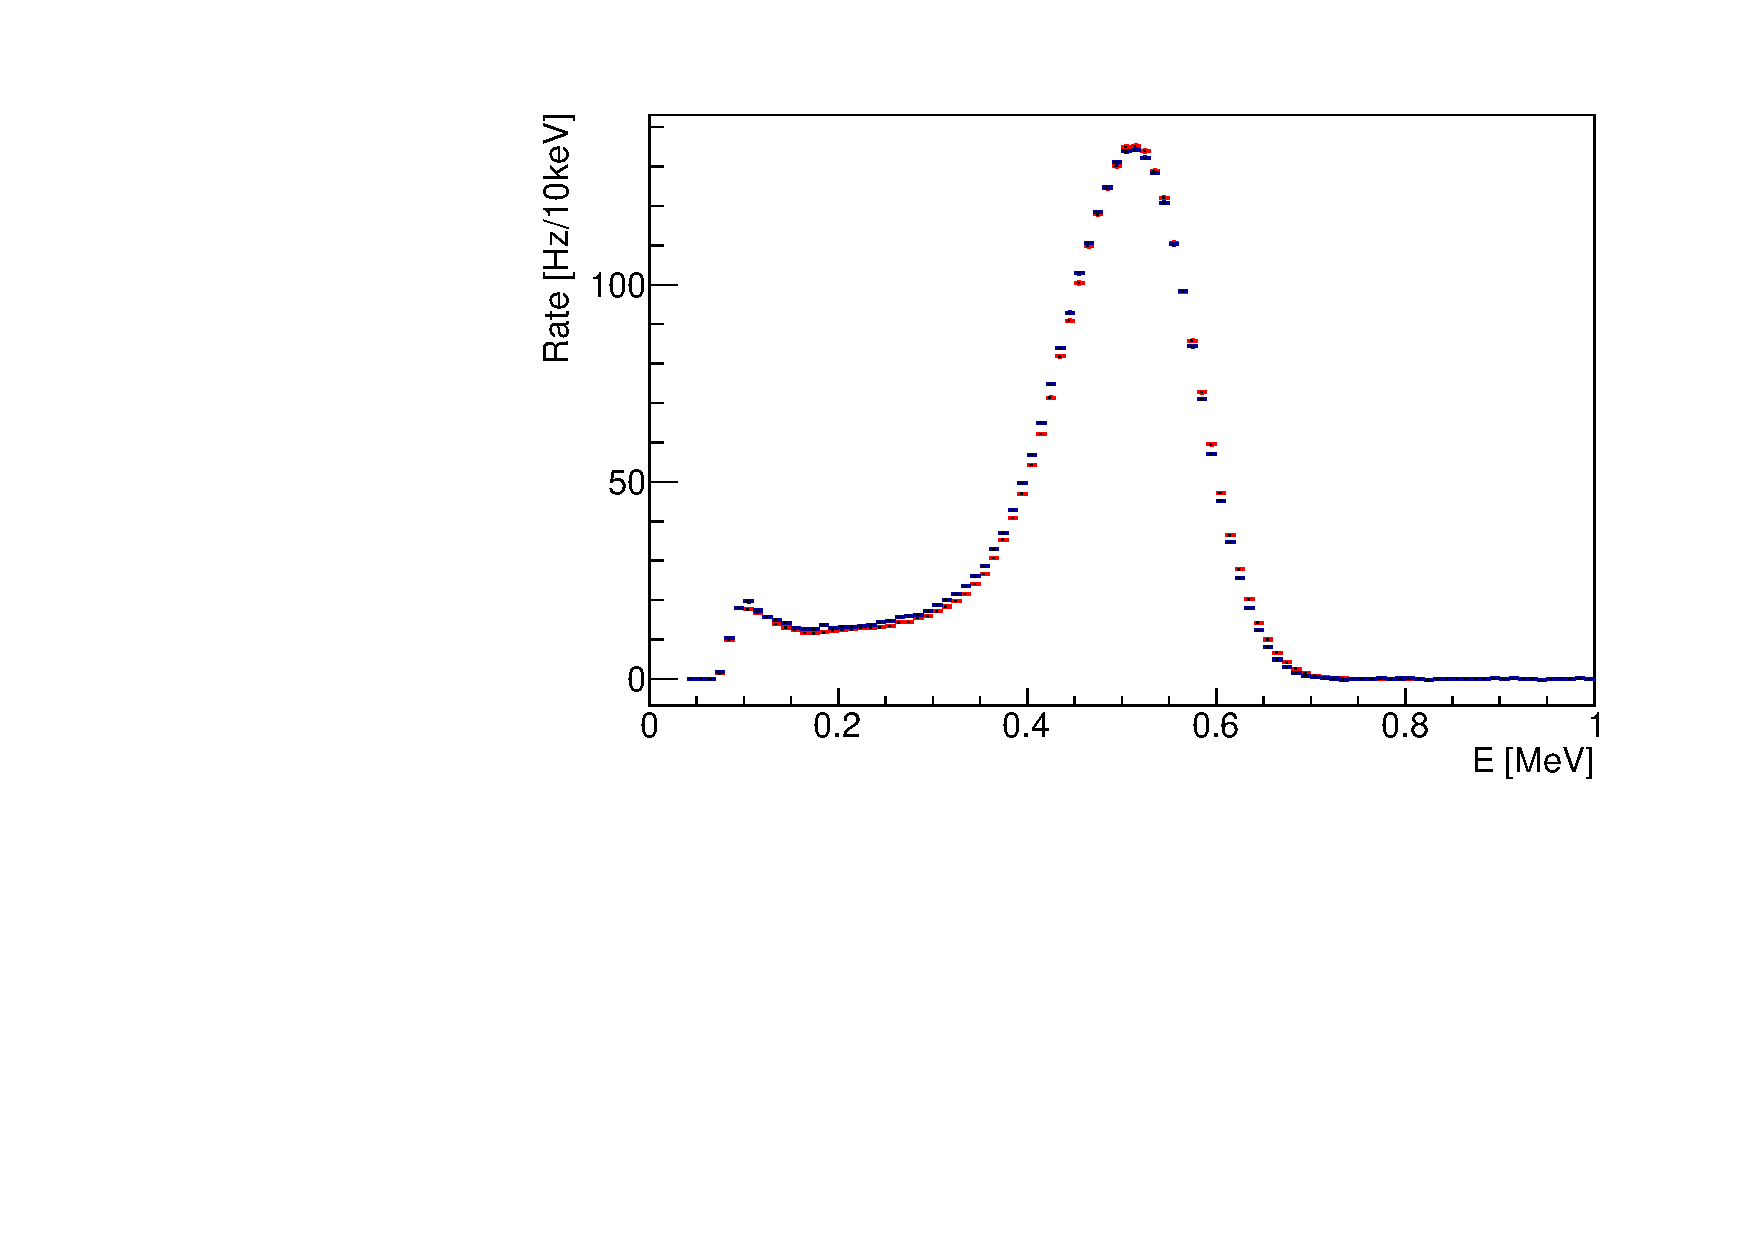
\includegraphics[width=60mm]{figures/hCs137v2.pdf}}\quad
\subfigure[Full detector MC-data for $^{22}$Na calibration.]{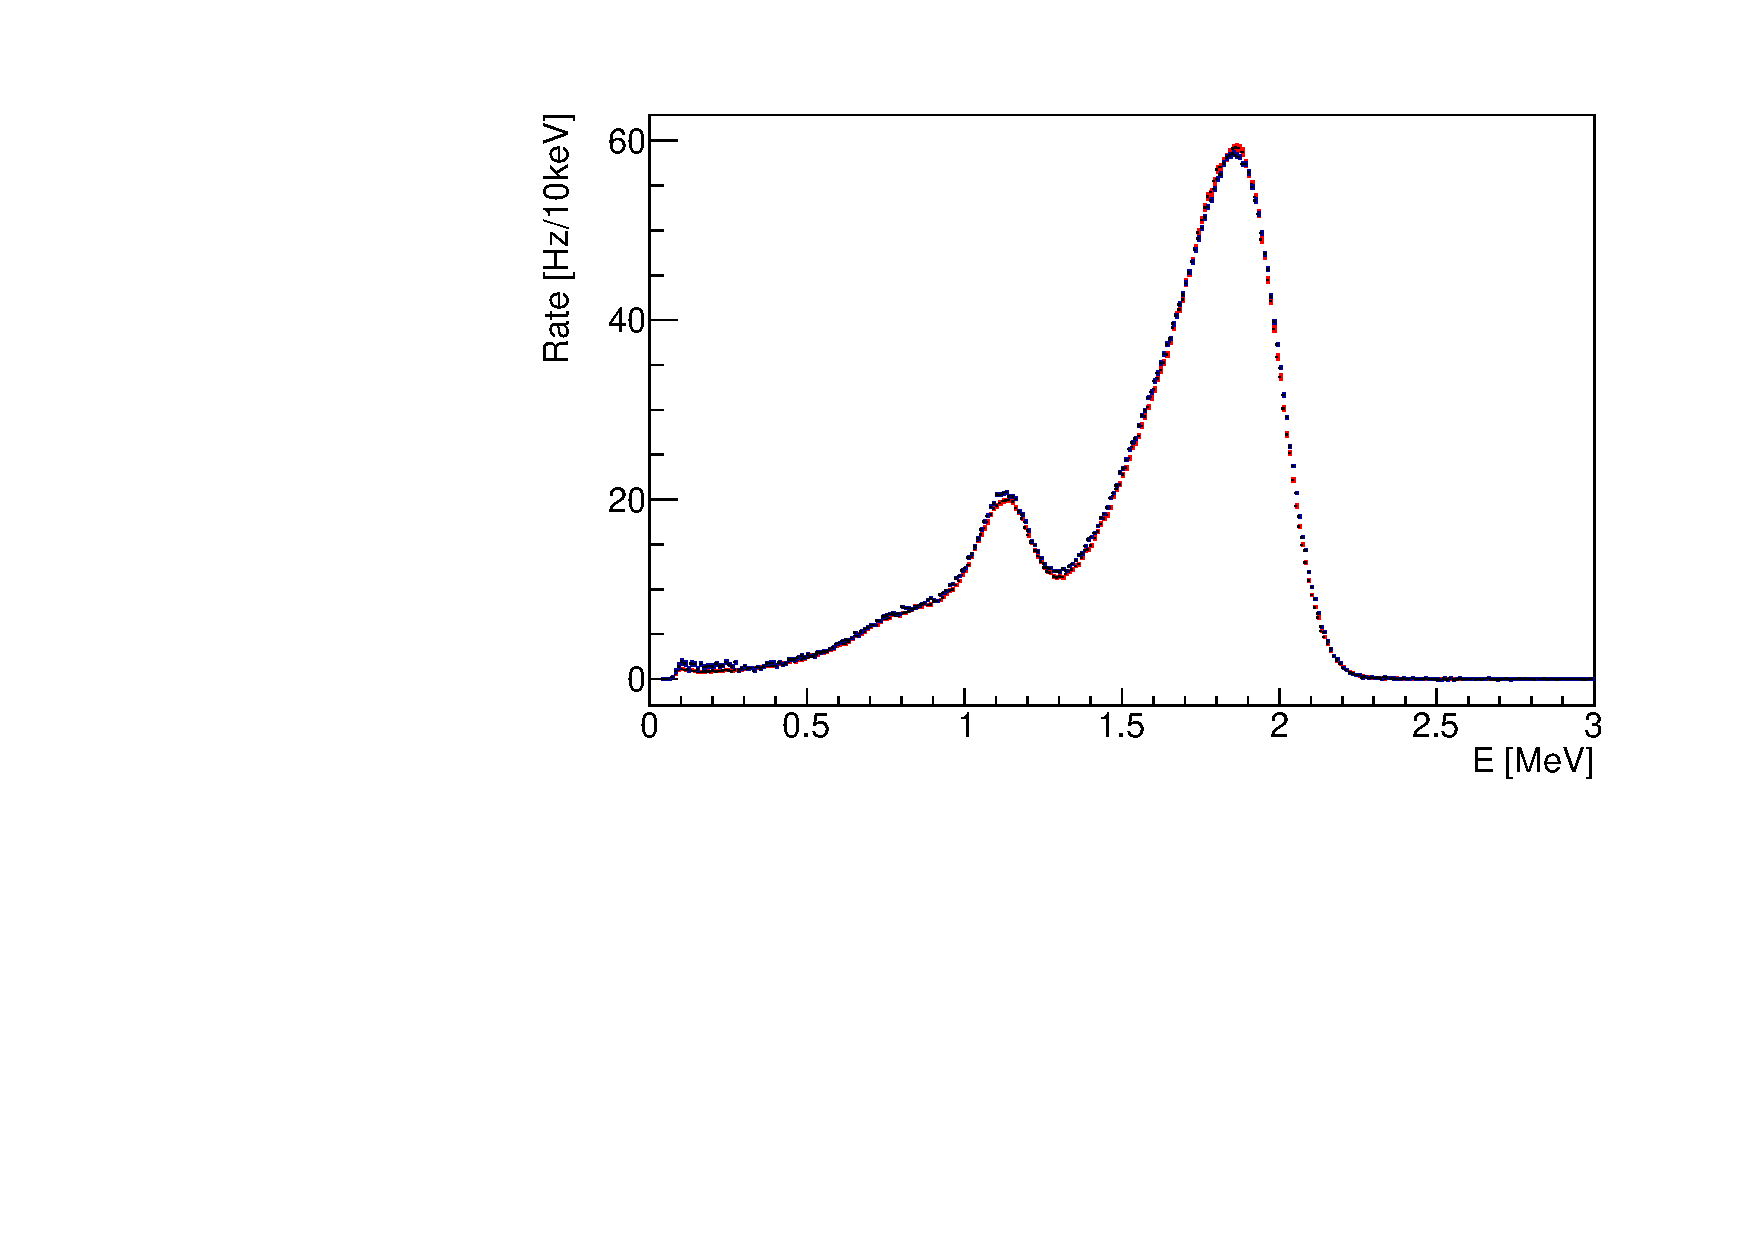
\includegraphics[width=60mm]{figures/hNa22v2.pdf}} \\
\subfigure[Full detector MC-data for $^{60}$Co calibration.]{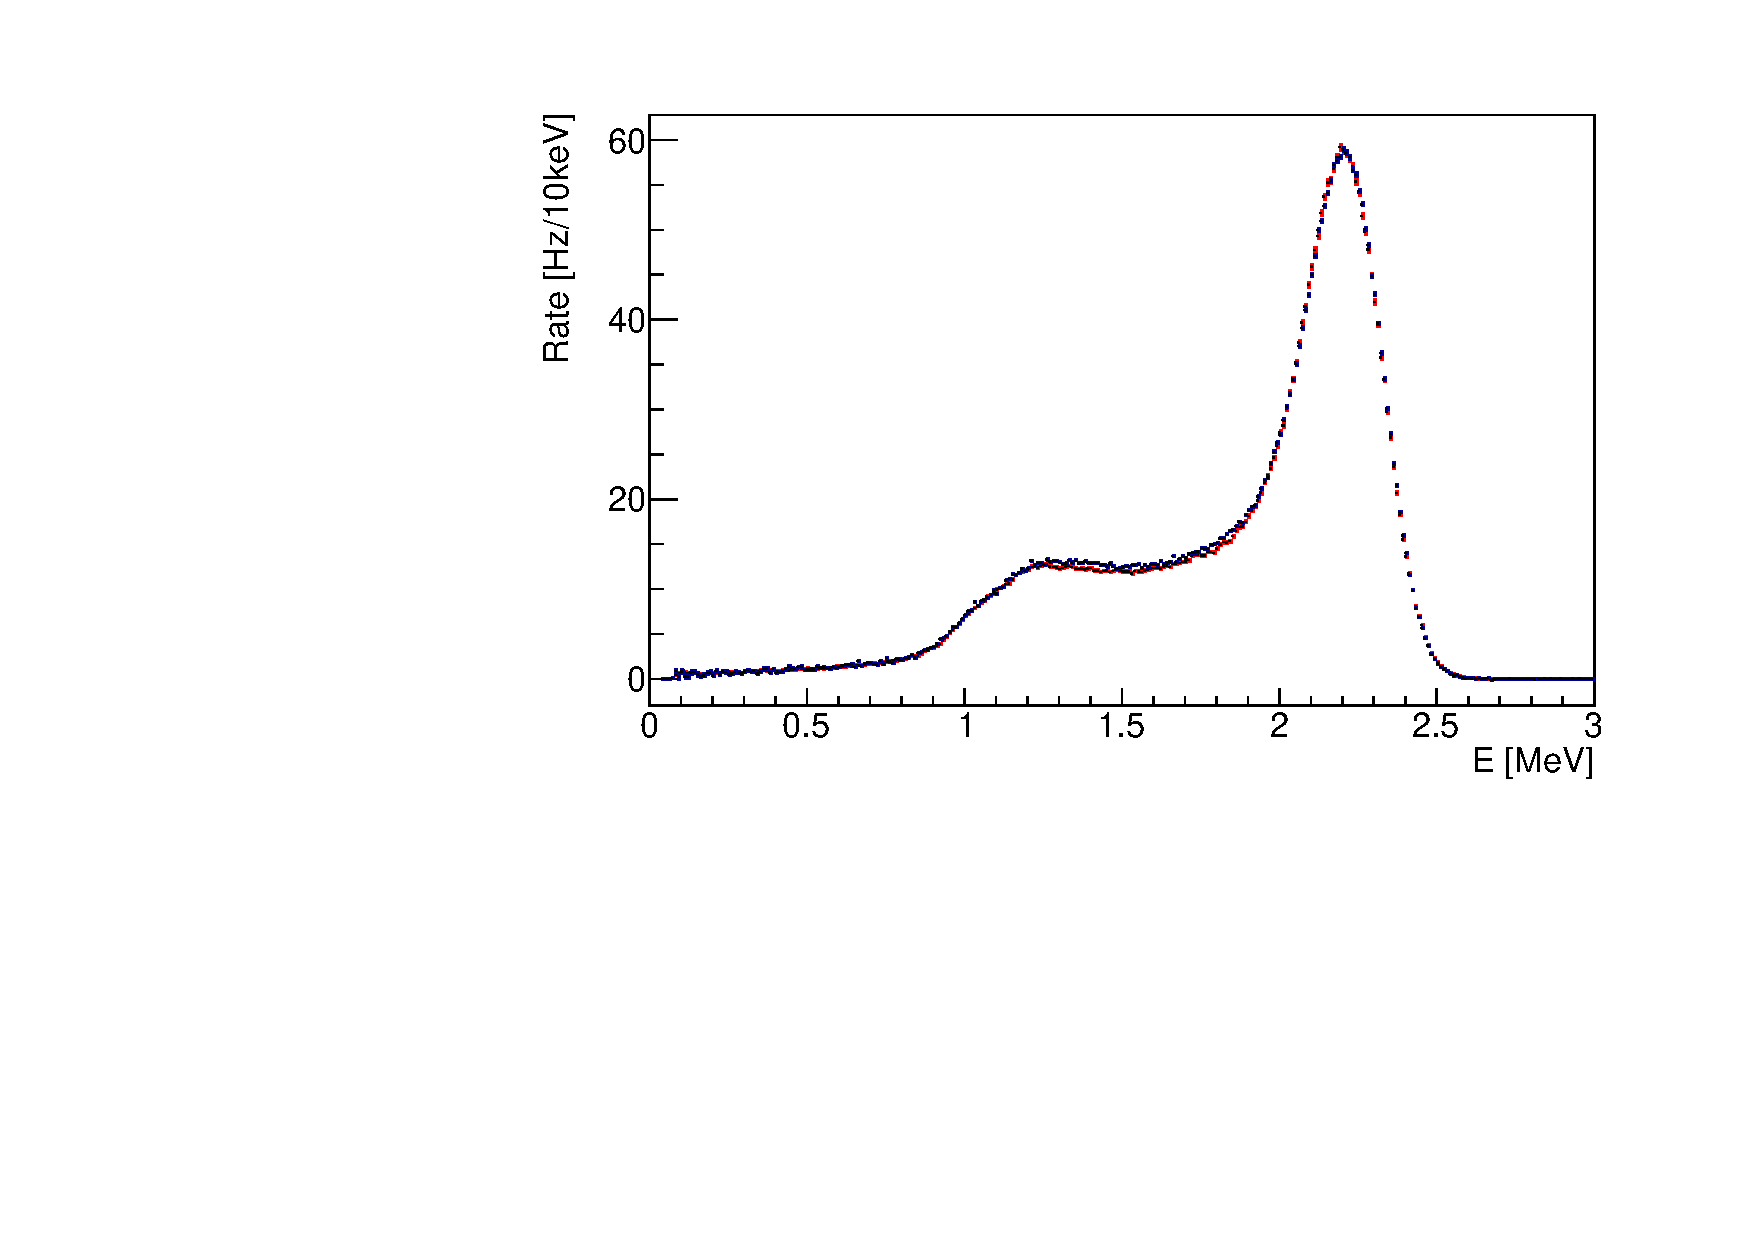
\includegraphics[width=60mm]{figures/hCo60v2.pdf}} \quad
\subfigure[Full detector MC-data for n-H capture gamma.]{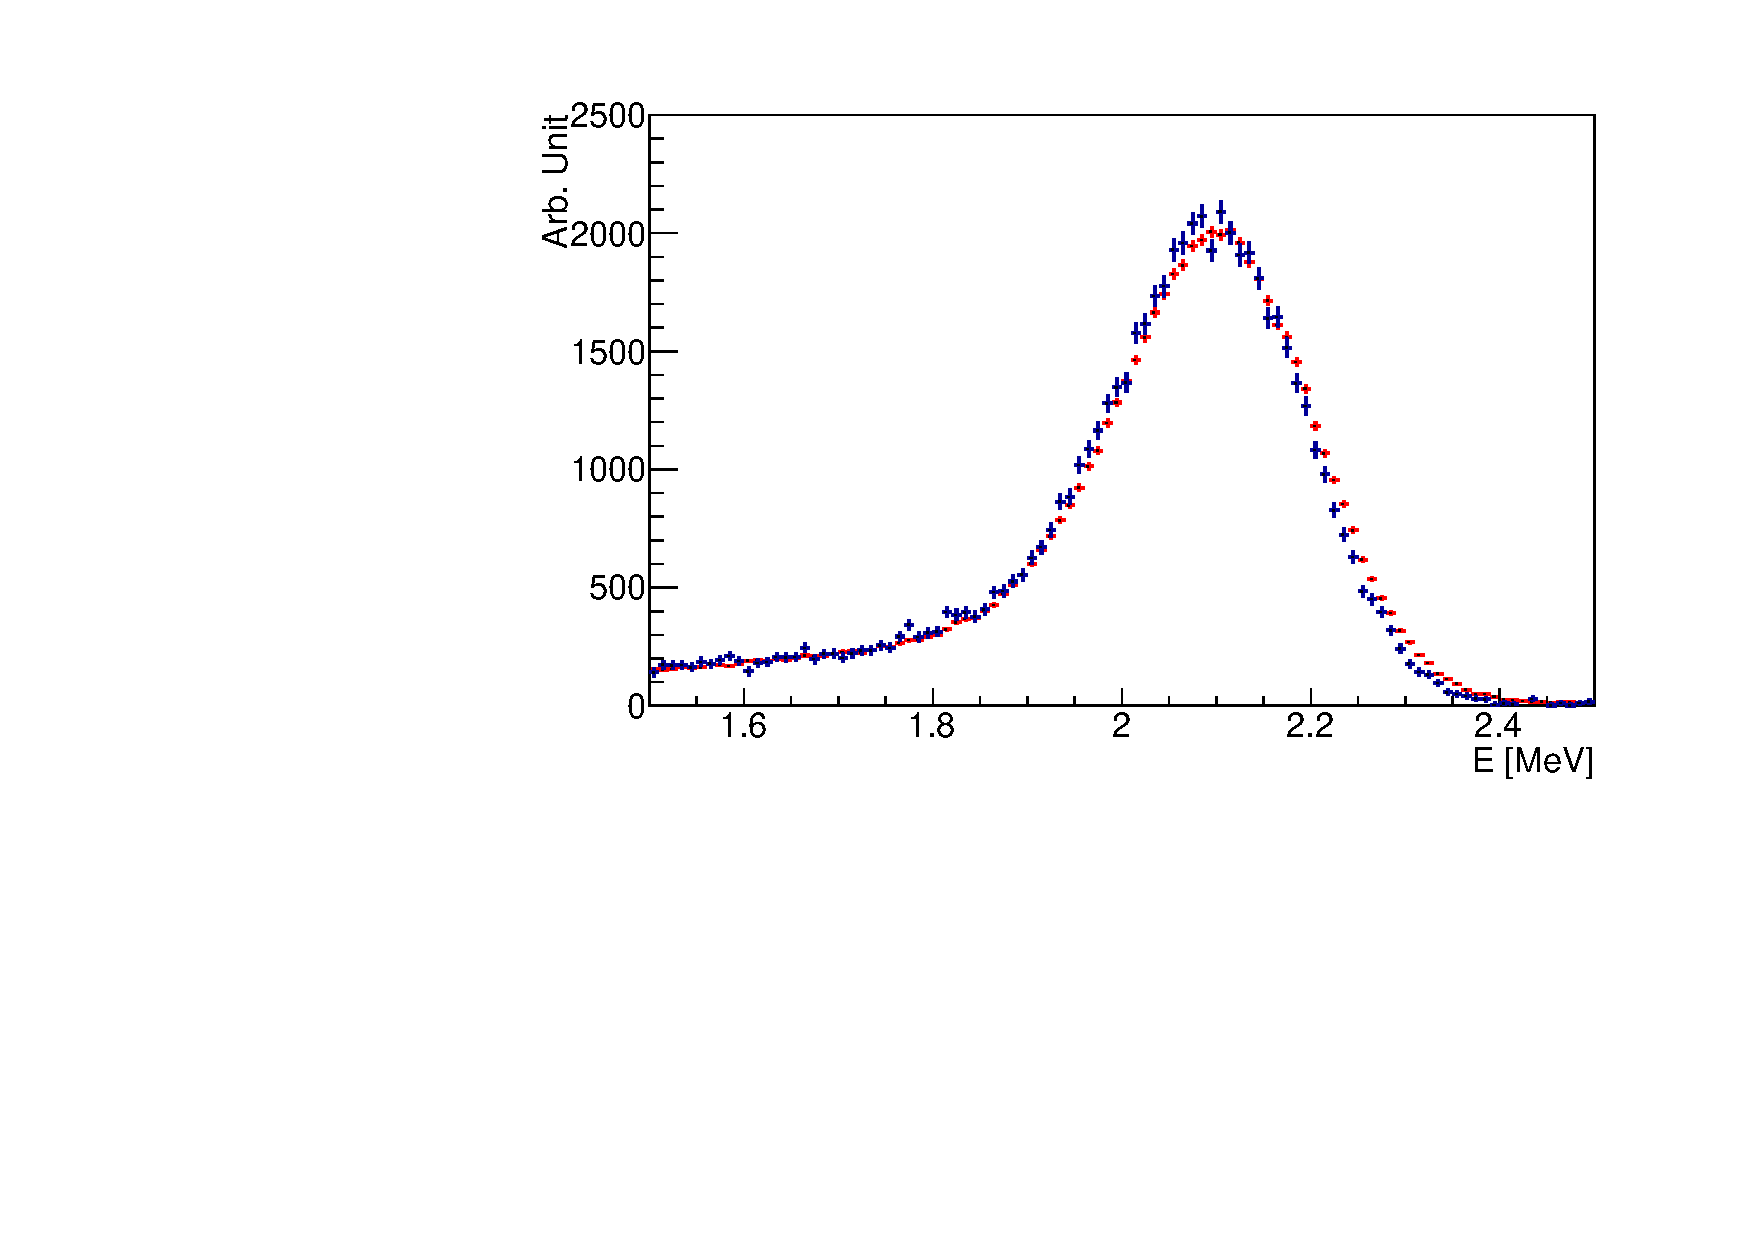
\includegraphics[width=60mm]{figures/hCf252v2.pdf}} \\
\subfigure[Full detector MC-data for $^{12}$B spectrum.]{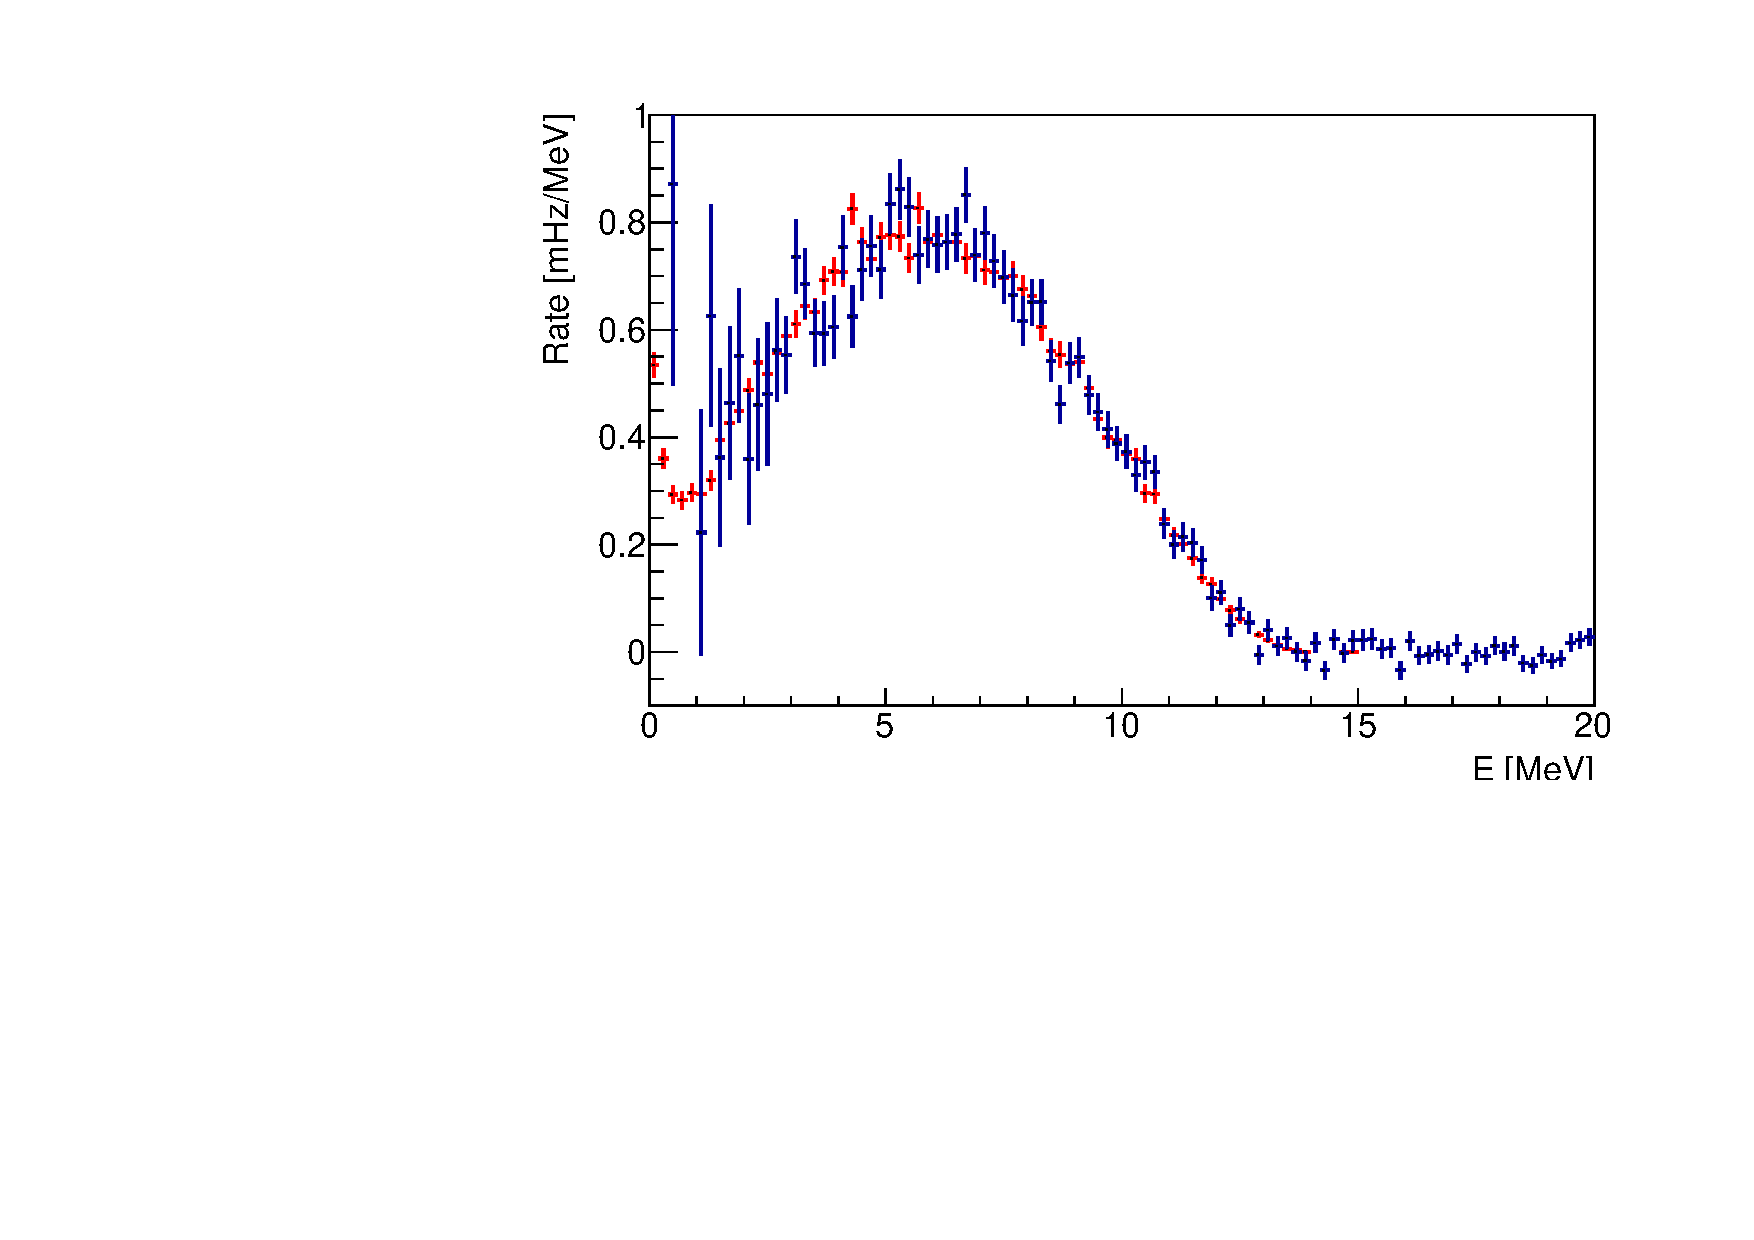
\includegraphics[width=60mm]{figures/hB12v2.pdf}}

\caption{The full detector calibration energy spectra data vs MC. comparison, showing only statisitical error. (red: MC, blue: data)}
\label{fig:goodfit2}
\end{figure}

\begin{figure}[h!]
\centering
\subfigure[Full detector MC-data for $^{137}$Cs calibration.]{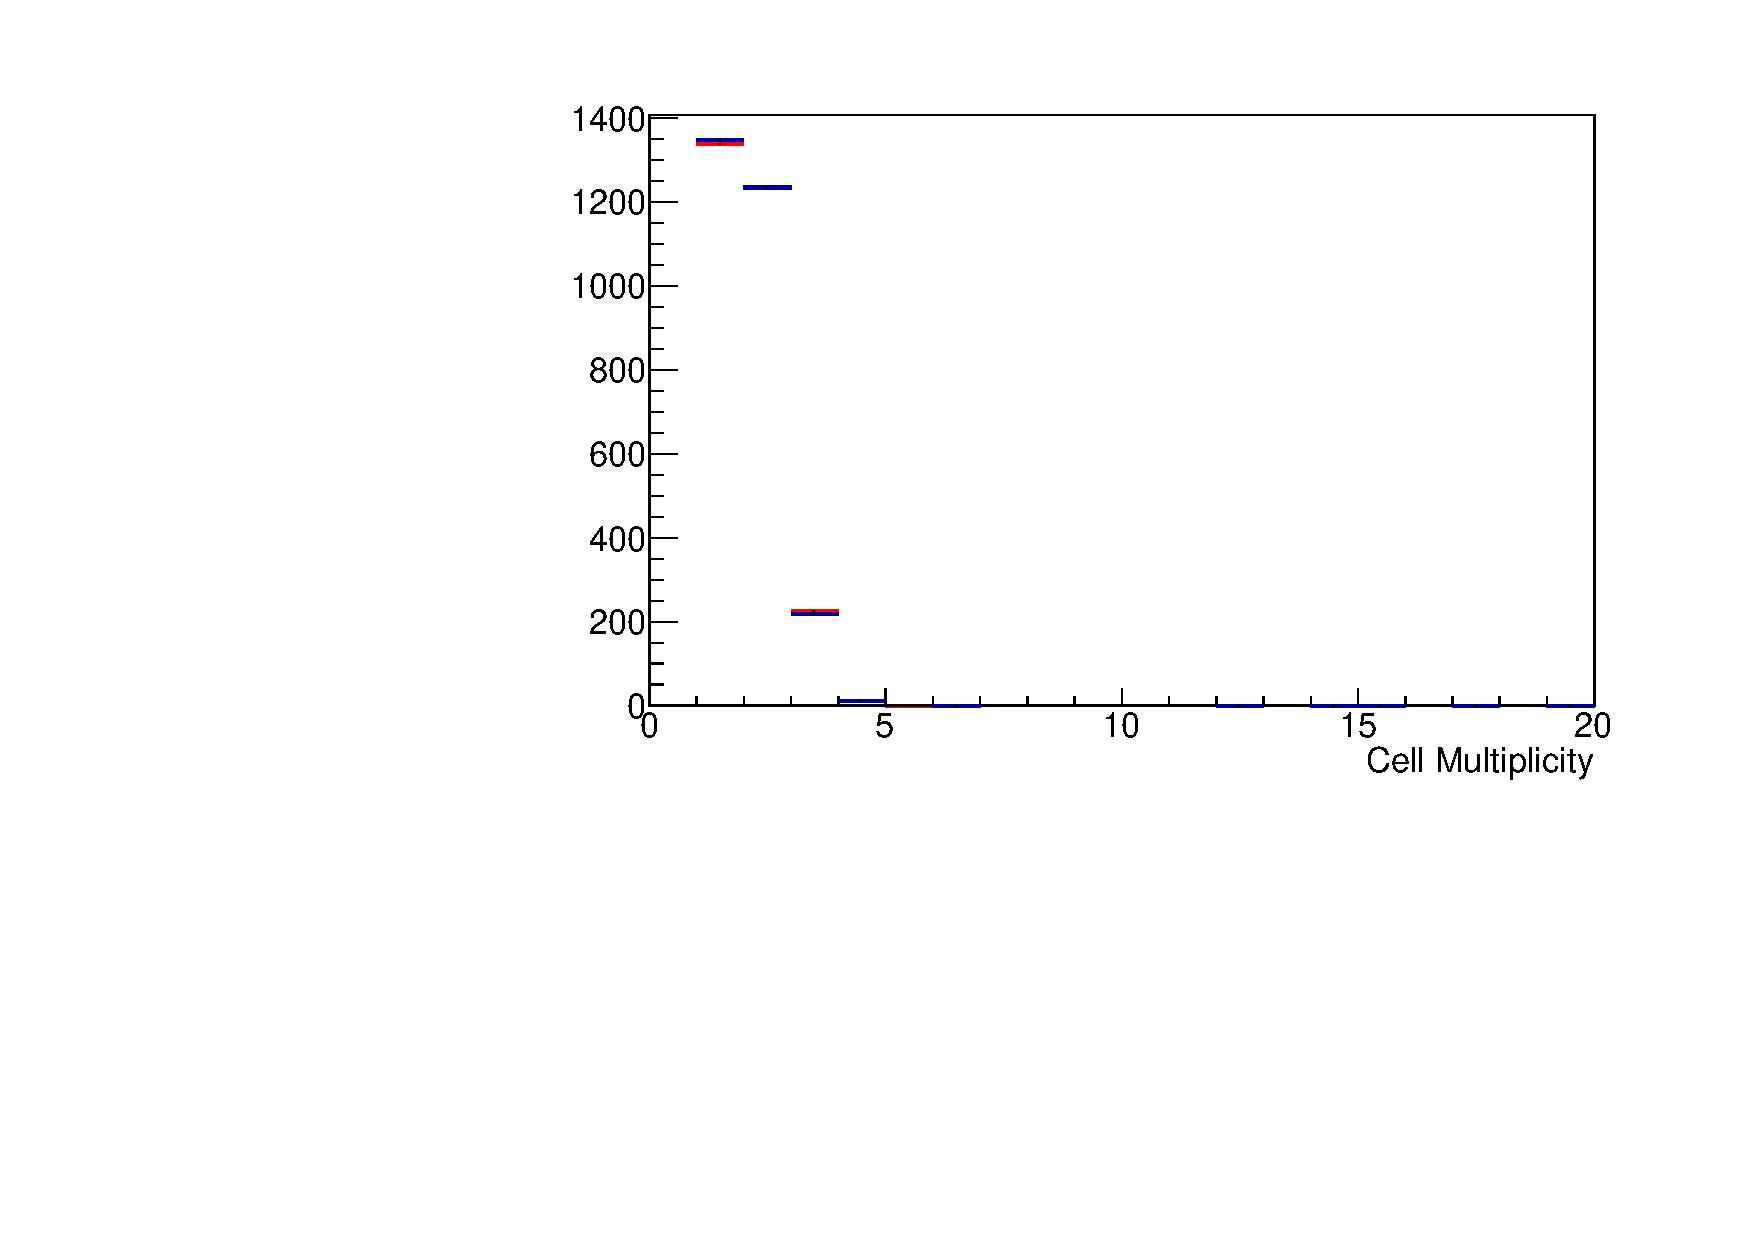
\includegraphics[width=60mm]{figures/hCs137multi.pdf}}\quad
\subfigure[Full detector MC-data for $^{22}$Na calibration.]{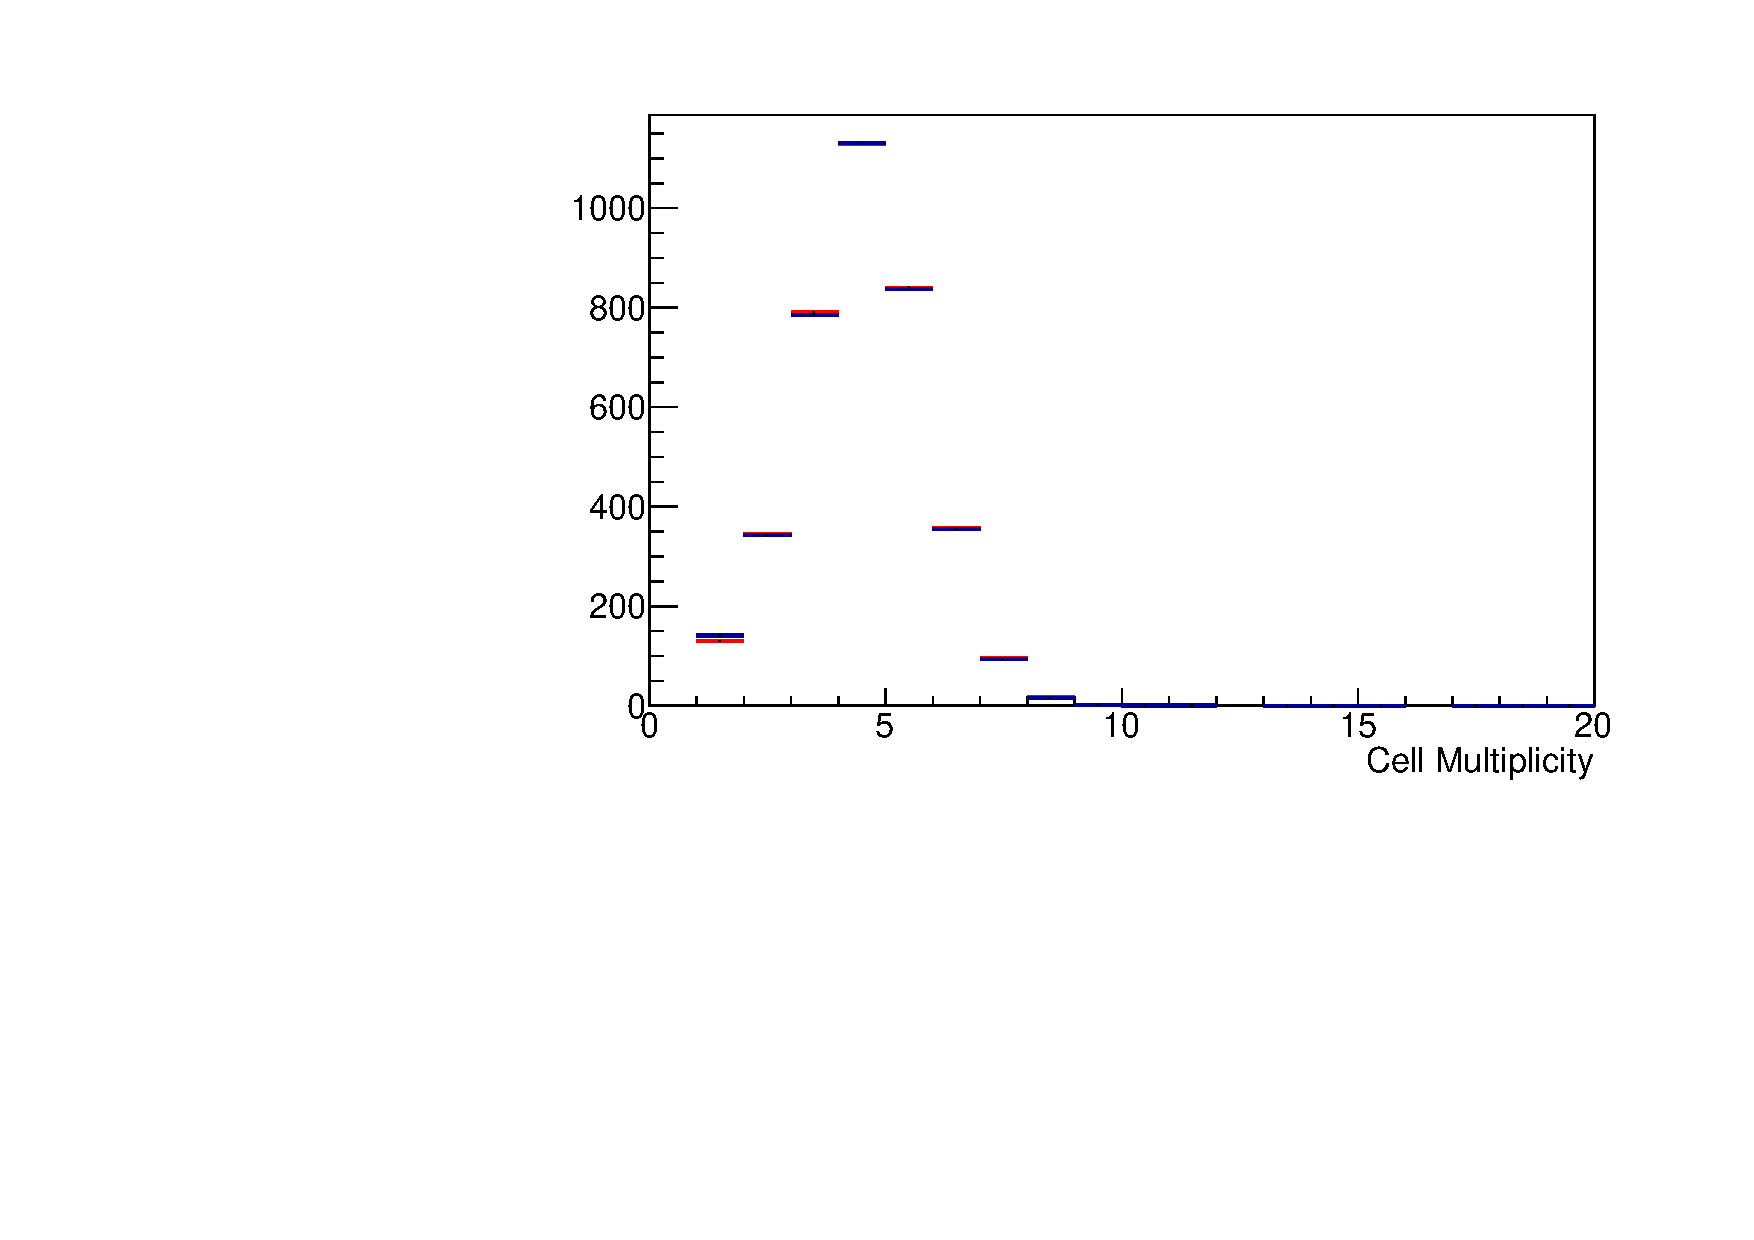
\includegraphics[width=60mm]{figures/hNa22mulit.pdf}} \\
\subfigure[Full detector MC-data for $^{60}$Co calibration.]{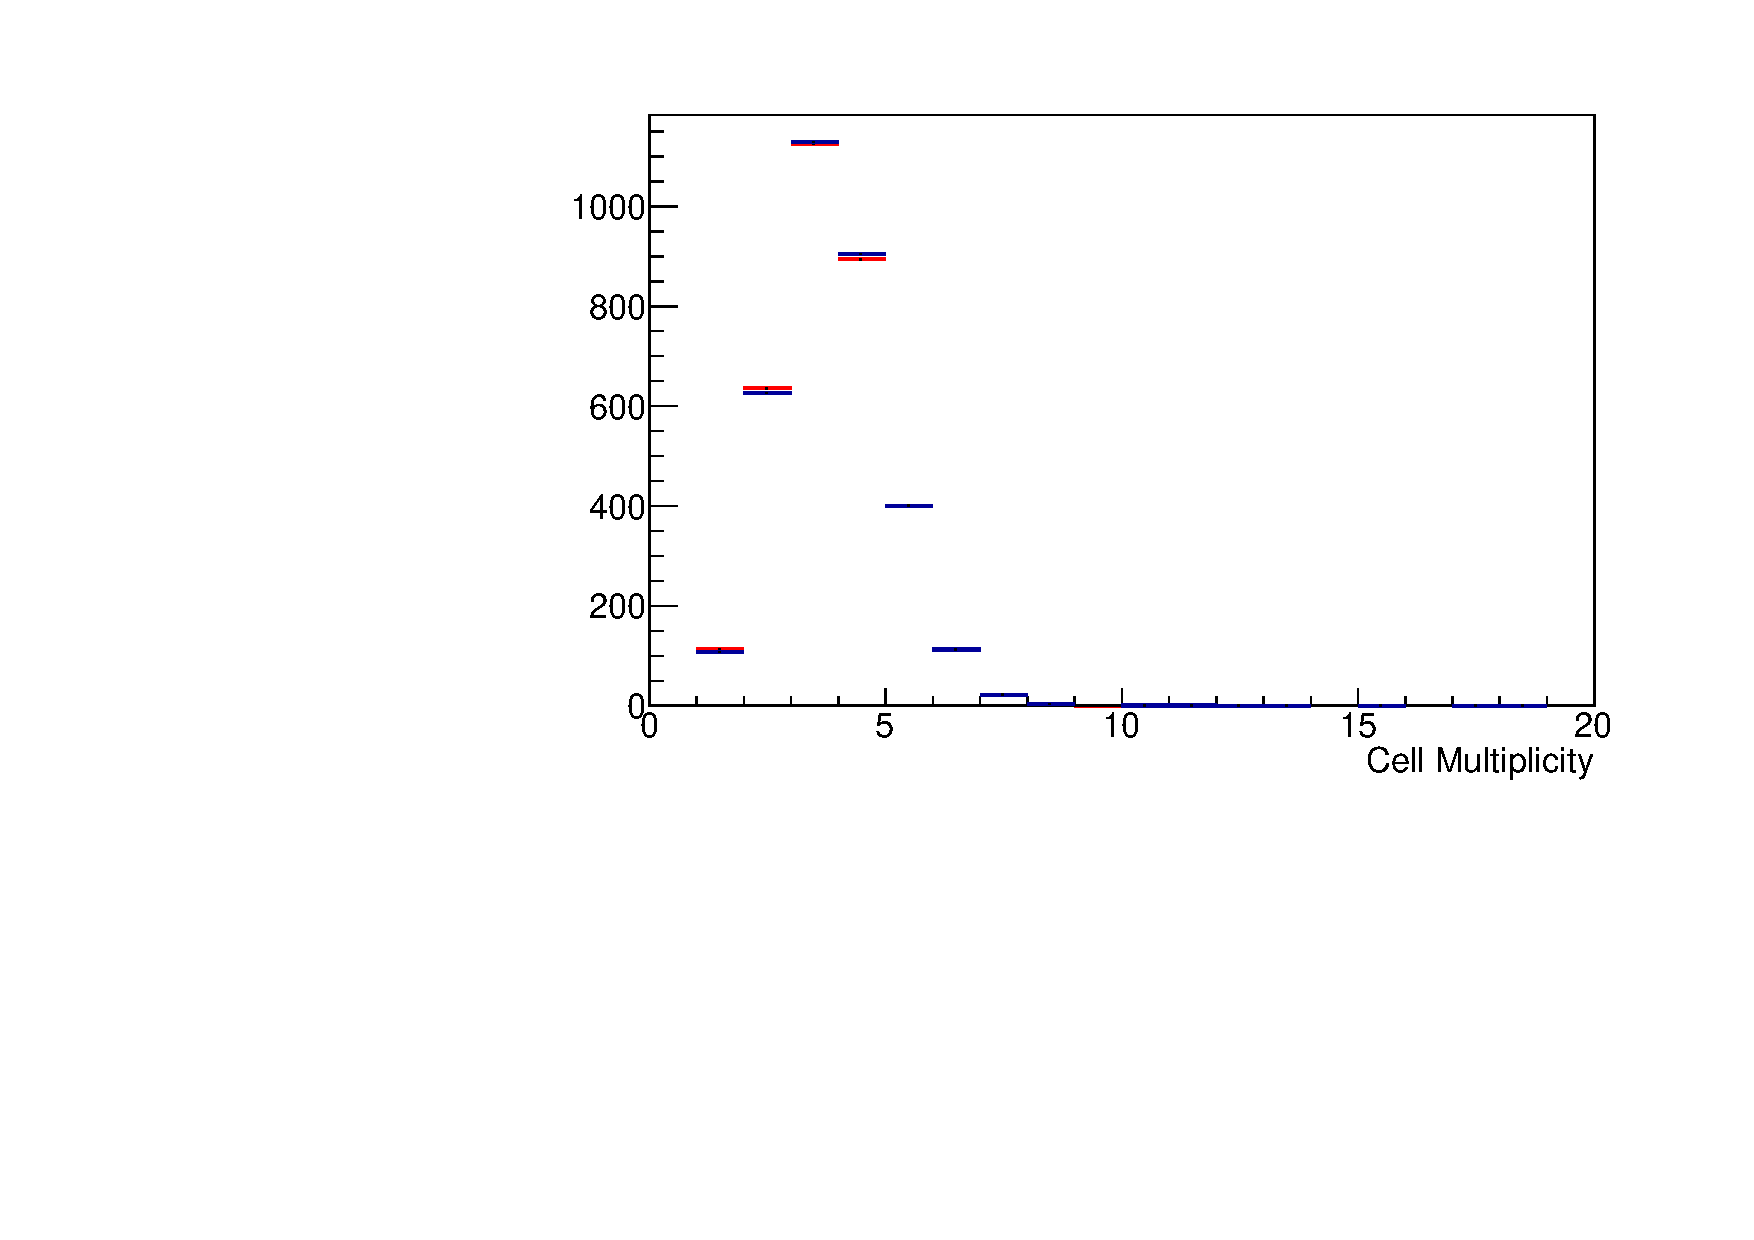
\includegraphics[width=60mm]{figures/hCo60multi.pdf}} 
\caption{Multiplicity distribution of gamma calibrations. (red: MC, blue: Data)}
\label{fig:multi}
\end{figure}

\begin{figure}[h!]
\centering
\subfigure[$\chi^2$ distribution depedent on first order Birks constant and Cherenkov efficiency.]{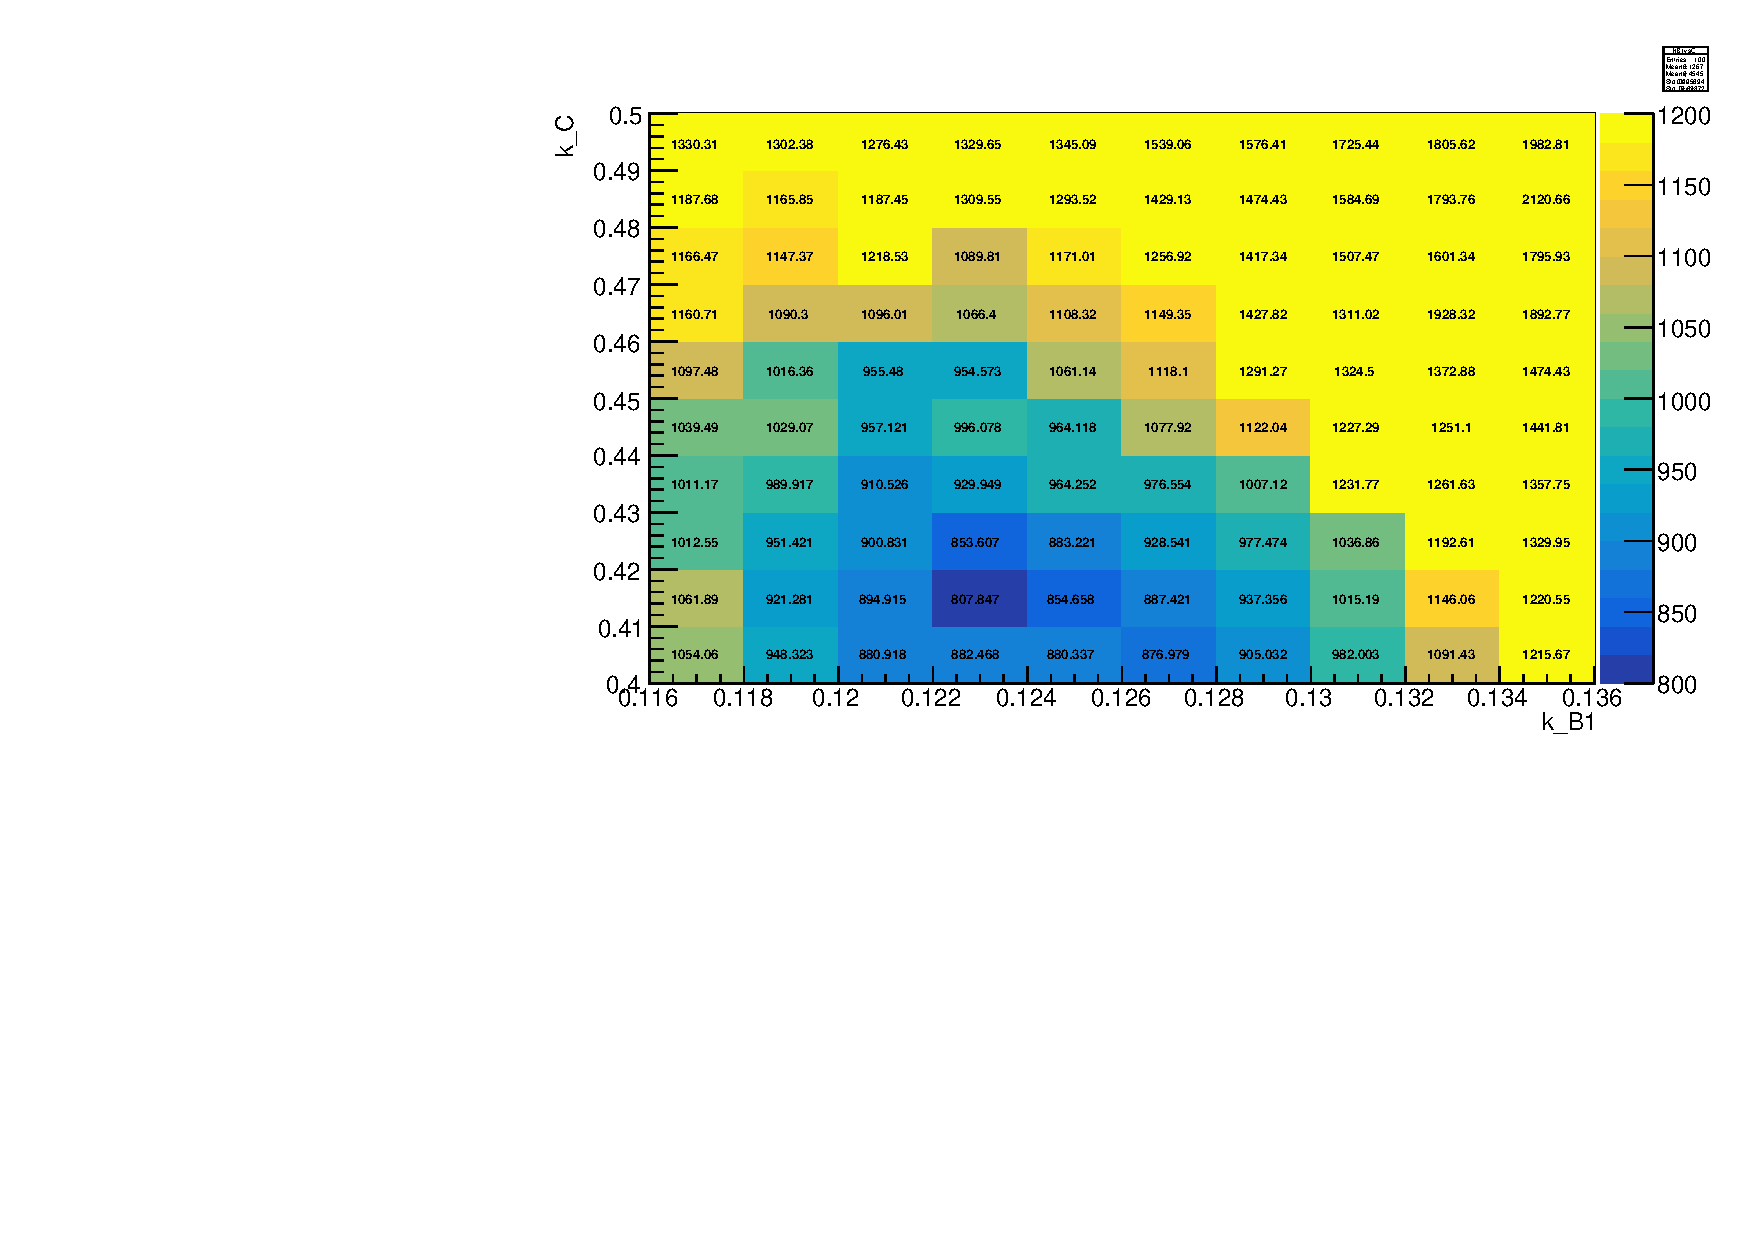
\includegraphics[width=70mm]{figures/k1vkc.pdf}}\quad
\subfigure[$\chi^2$ distribution depedent on first order and second order Birks constant.]{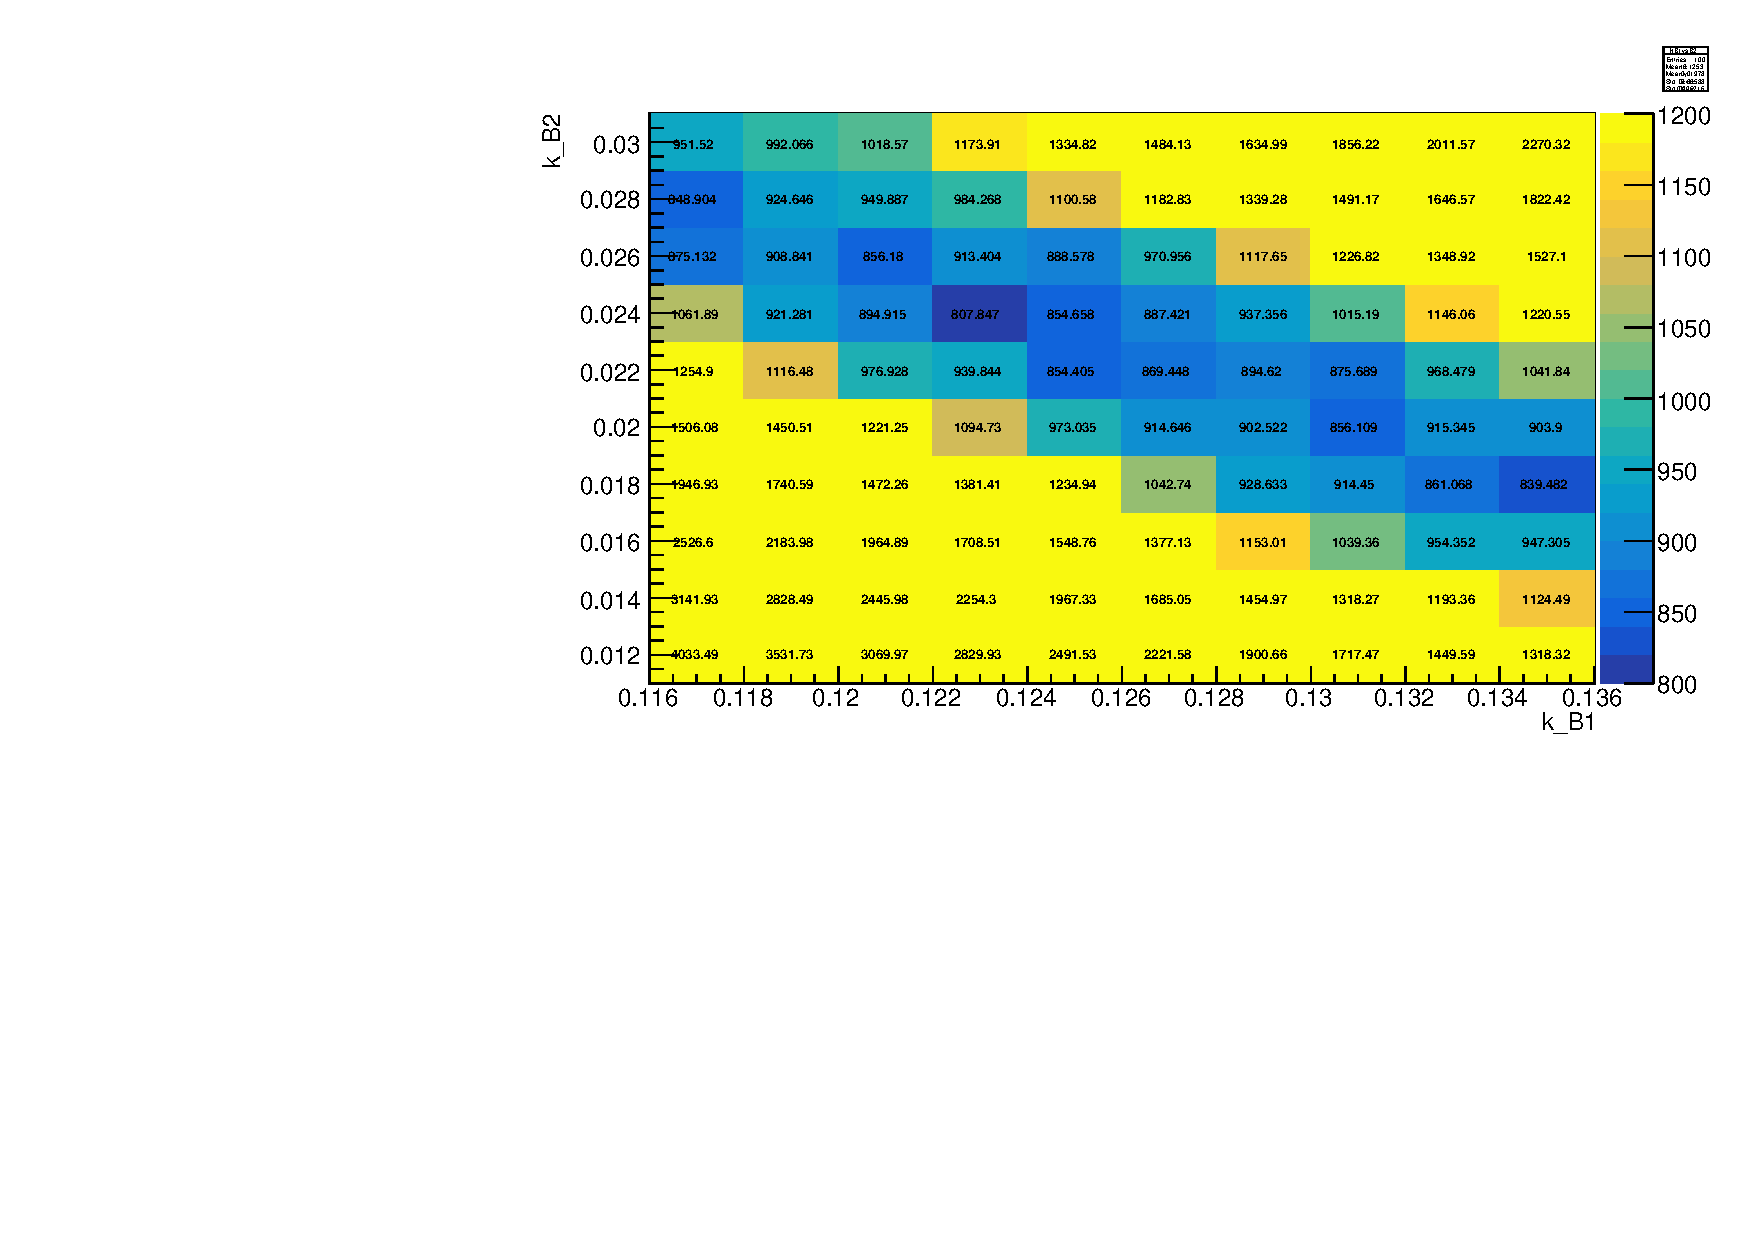
\includegraphics[width=70mm]{figures/k1vk2.pdf}} \\
\subfigure[$\chi^2$ distribution depedent on second order and Birks constant and Cherenkov efficiency.]{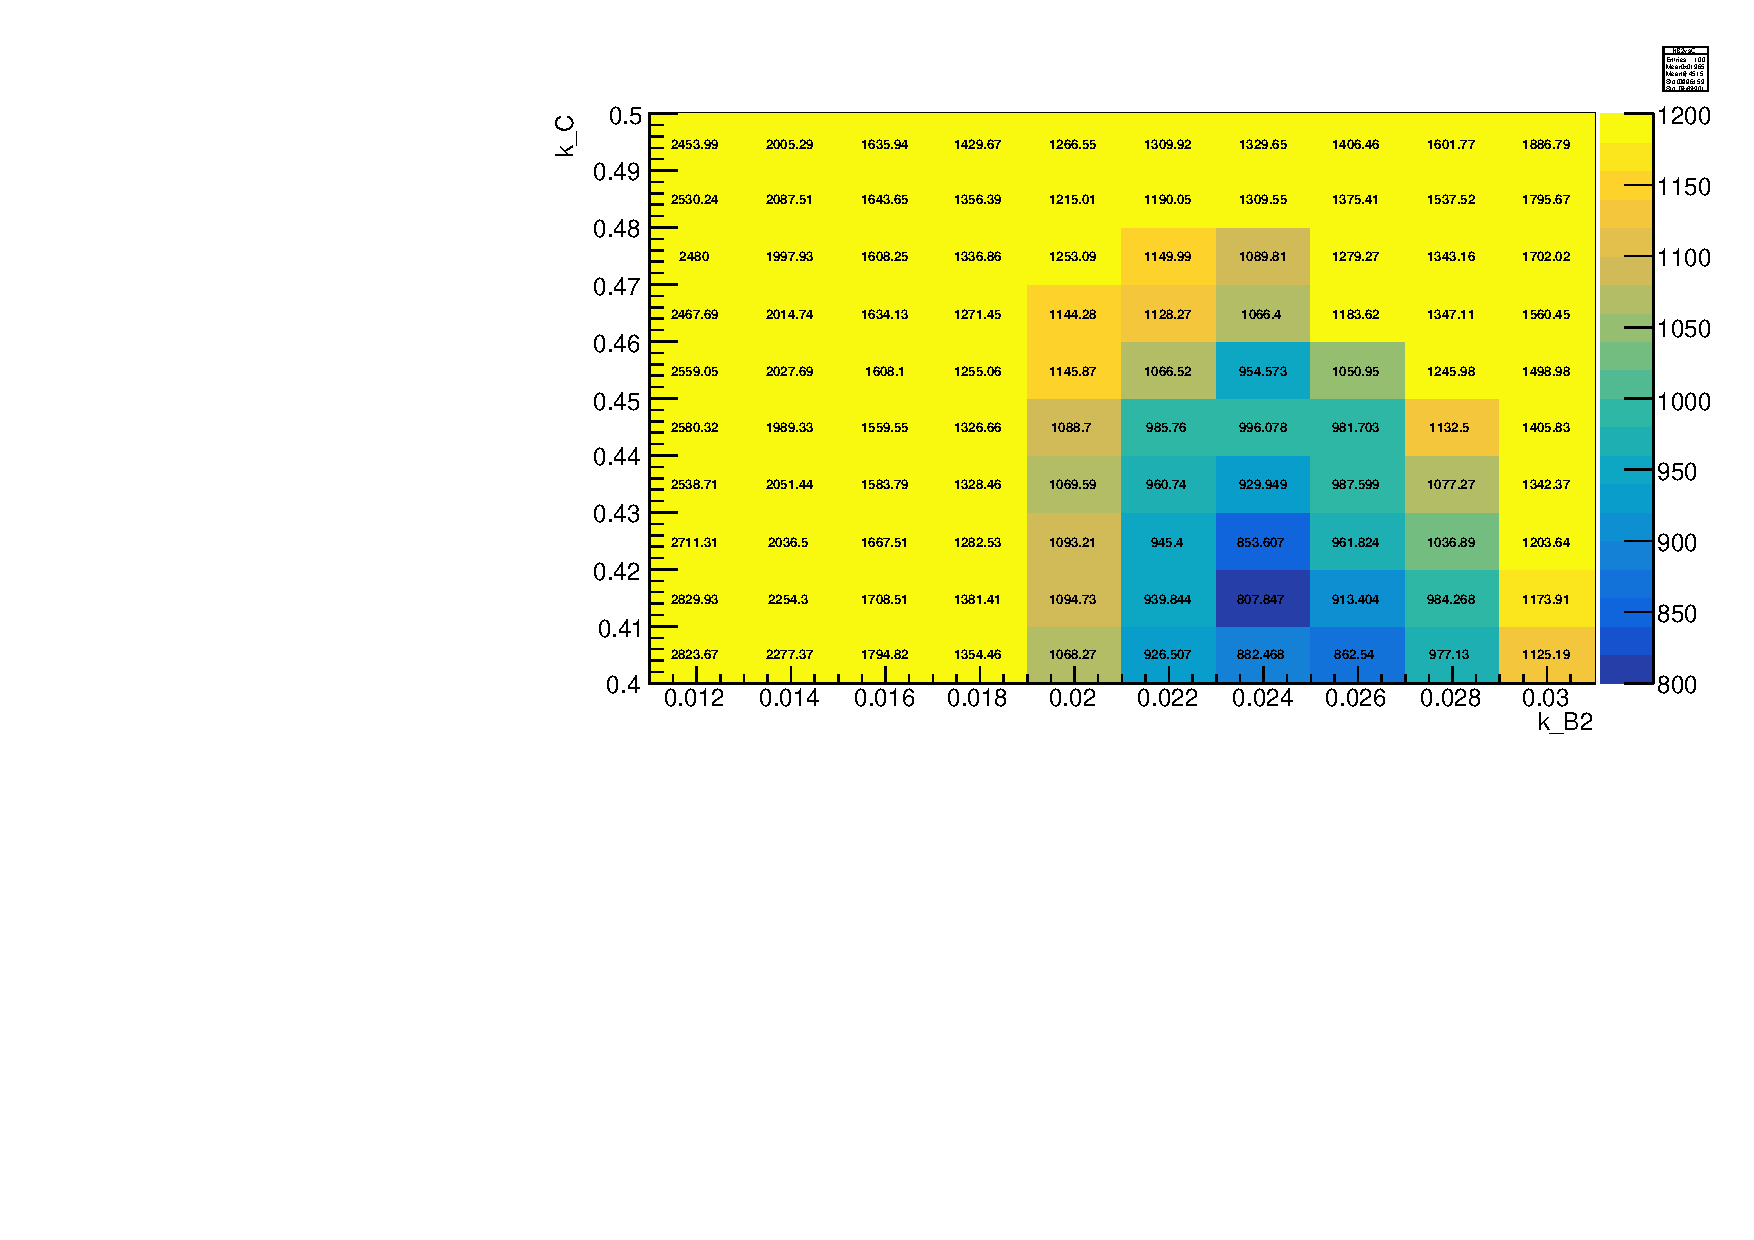
\includegraphics[width=70mm]{figures/k2vkc.pdf}} 
\caption{$\chi^2$ distribution with respect to the values of nonlinearity parameters.}
\label{fig:chi2}
\end{figure}
\newpage
\clearpage

\subsection{Single Cell Spectrum Comparison}
\label{sec:single}
The comparing the calibration spectra measured by only the single detector cells that are mostly adjacent to the calibration source can minimize the detector geometry correlated and the 85 keV thresholding effect for us to study LS nonlinearity.
The data and MC agreemnt in single-cell reconstructed energy is a good cross check of the full-detector best fit model.

Hence, we collected the single compton scattering gamma energy measured by only the single cells adjacent to the calibration sources respectively, four cells per source.
To reduce the systematic difference of energy scale between cells, the single hit gamma spectra from four cells were represented by the average spectrum of them. 
In gamma radioactive calibrations, the range of interest were from 0.2 MeV to the ends of spectra.
The range of fitting for gamma spectrum from n-H capture was 1.5 MeV to 2.3 MeV.
In single cell comparison, we compare only the single hit $^{12}$B electron energy spectrum.
The range of fitting for $^{12}$B spectrum is 3 to 13.5 MeV. 
To simplify the fitting, the MC spectra were normalized to data based on the spectral integral in the range of interest.
We performed the $\chi^2$ comparison to each of the calibraion spectra, and treat the sum of the $\chi^2$ values as combined $\chi^2$. 

The data vs. MC comparisons with full detector best fit are shown in Figure \ref{fig:goodfit}. 
The $\chi^2/NDF = 1425.4/584$ with the parameters nonlinearity model obtained in the full-detector fitting in Section \ref{sec:fulldet}, the overall energy shift is $\beta_{rec} = 0.40\%$.

\begin{figure}[h!]
\centering
\subfigure[Best-fit MC-data for $^{137}$Cs calibration.]{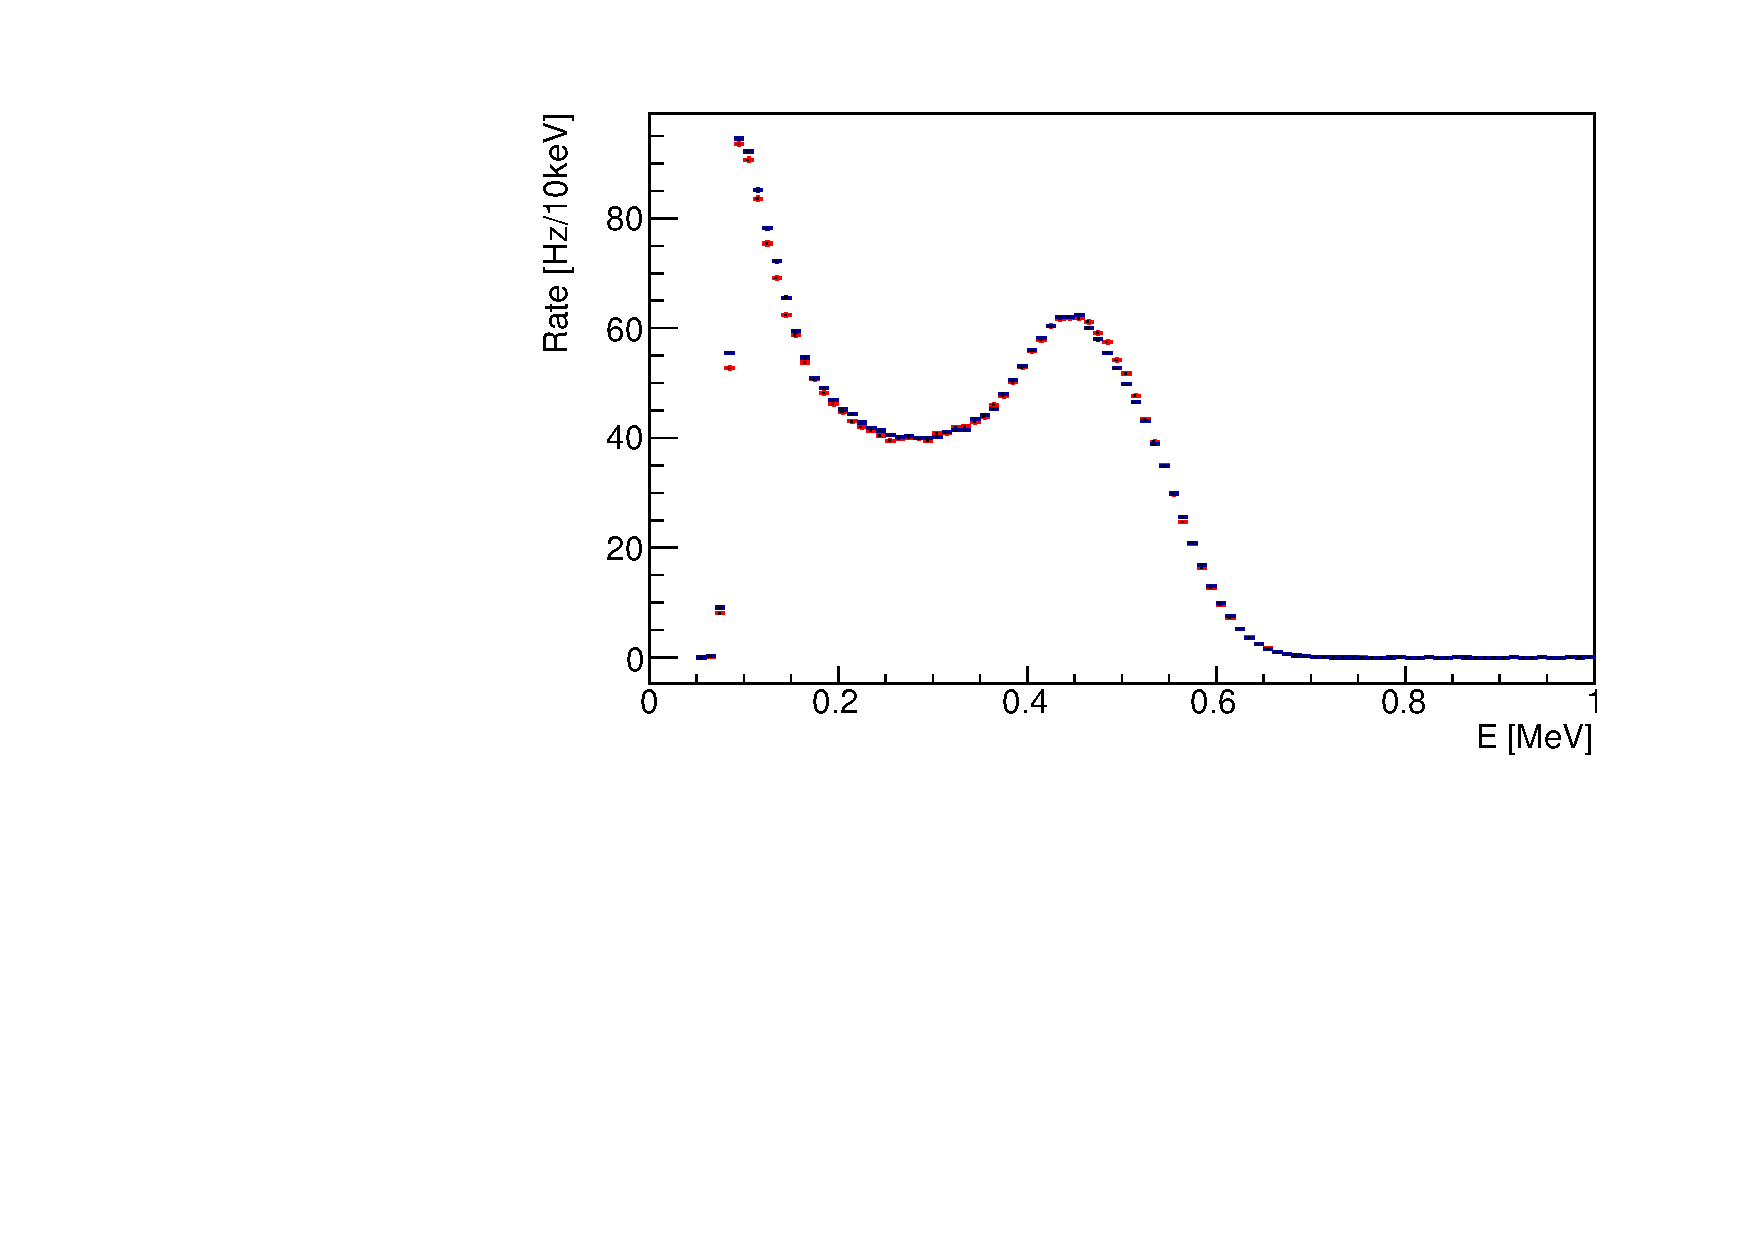
\includegraphics[width=60mm]{figures/hCs137v2single.pdf}}\quad
\subfigure[Best-fit MC-data for $^{22}$Na calibration.]{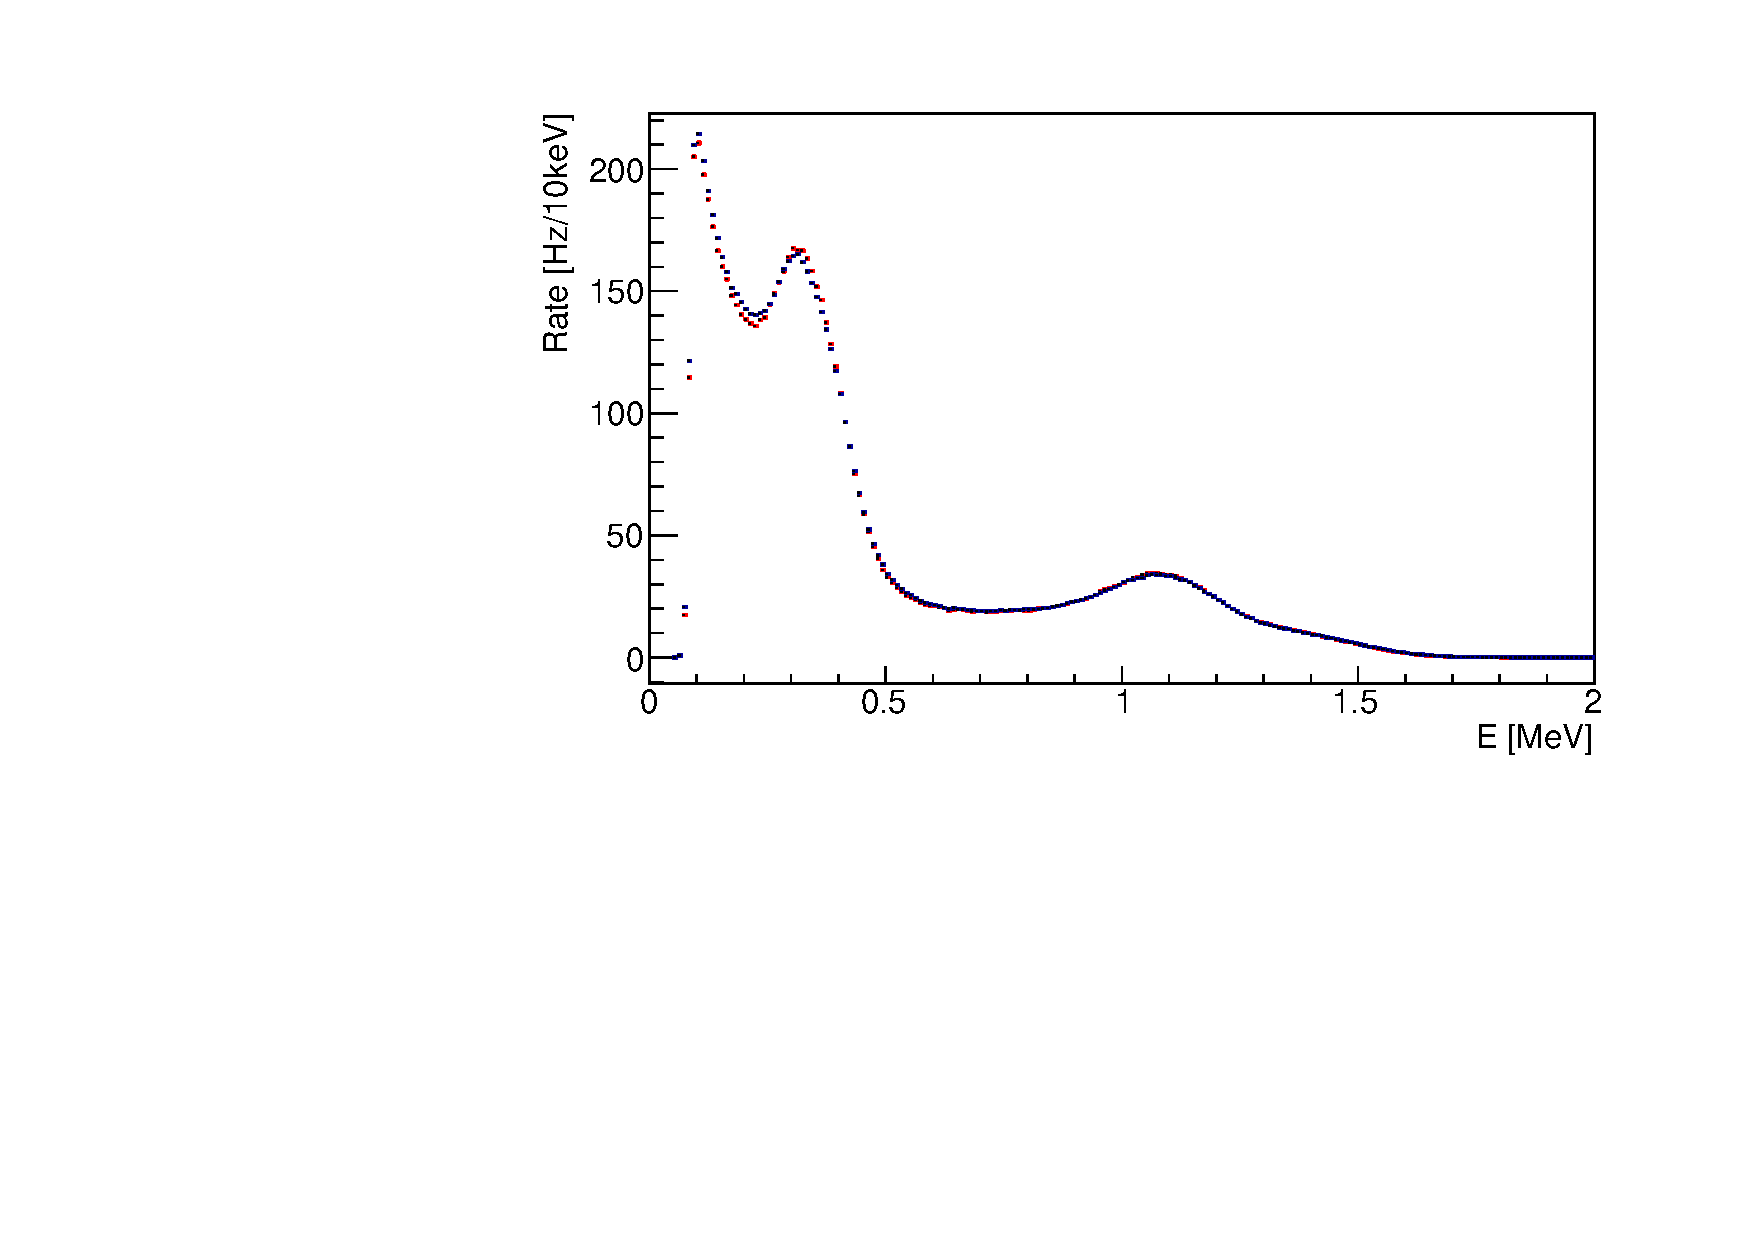
\includegraphics[width=60mm]{figures/hNa22v2single.pdf}} \\
\subfigure[Best-fit MC-data for $^{60}$Co calibration.]{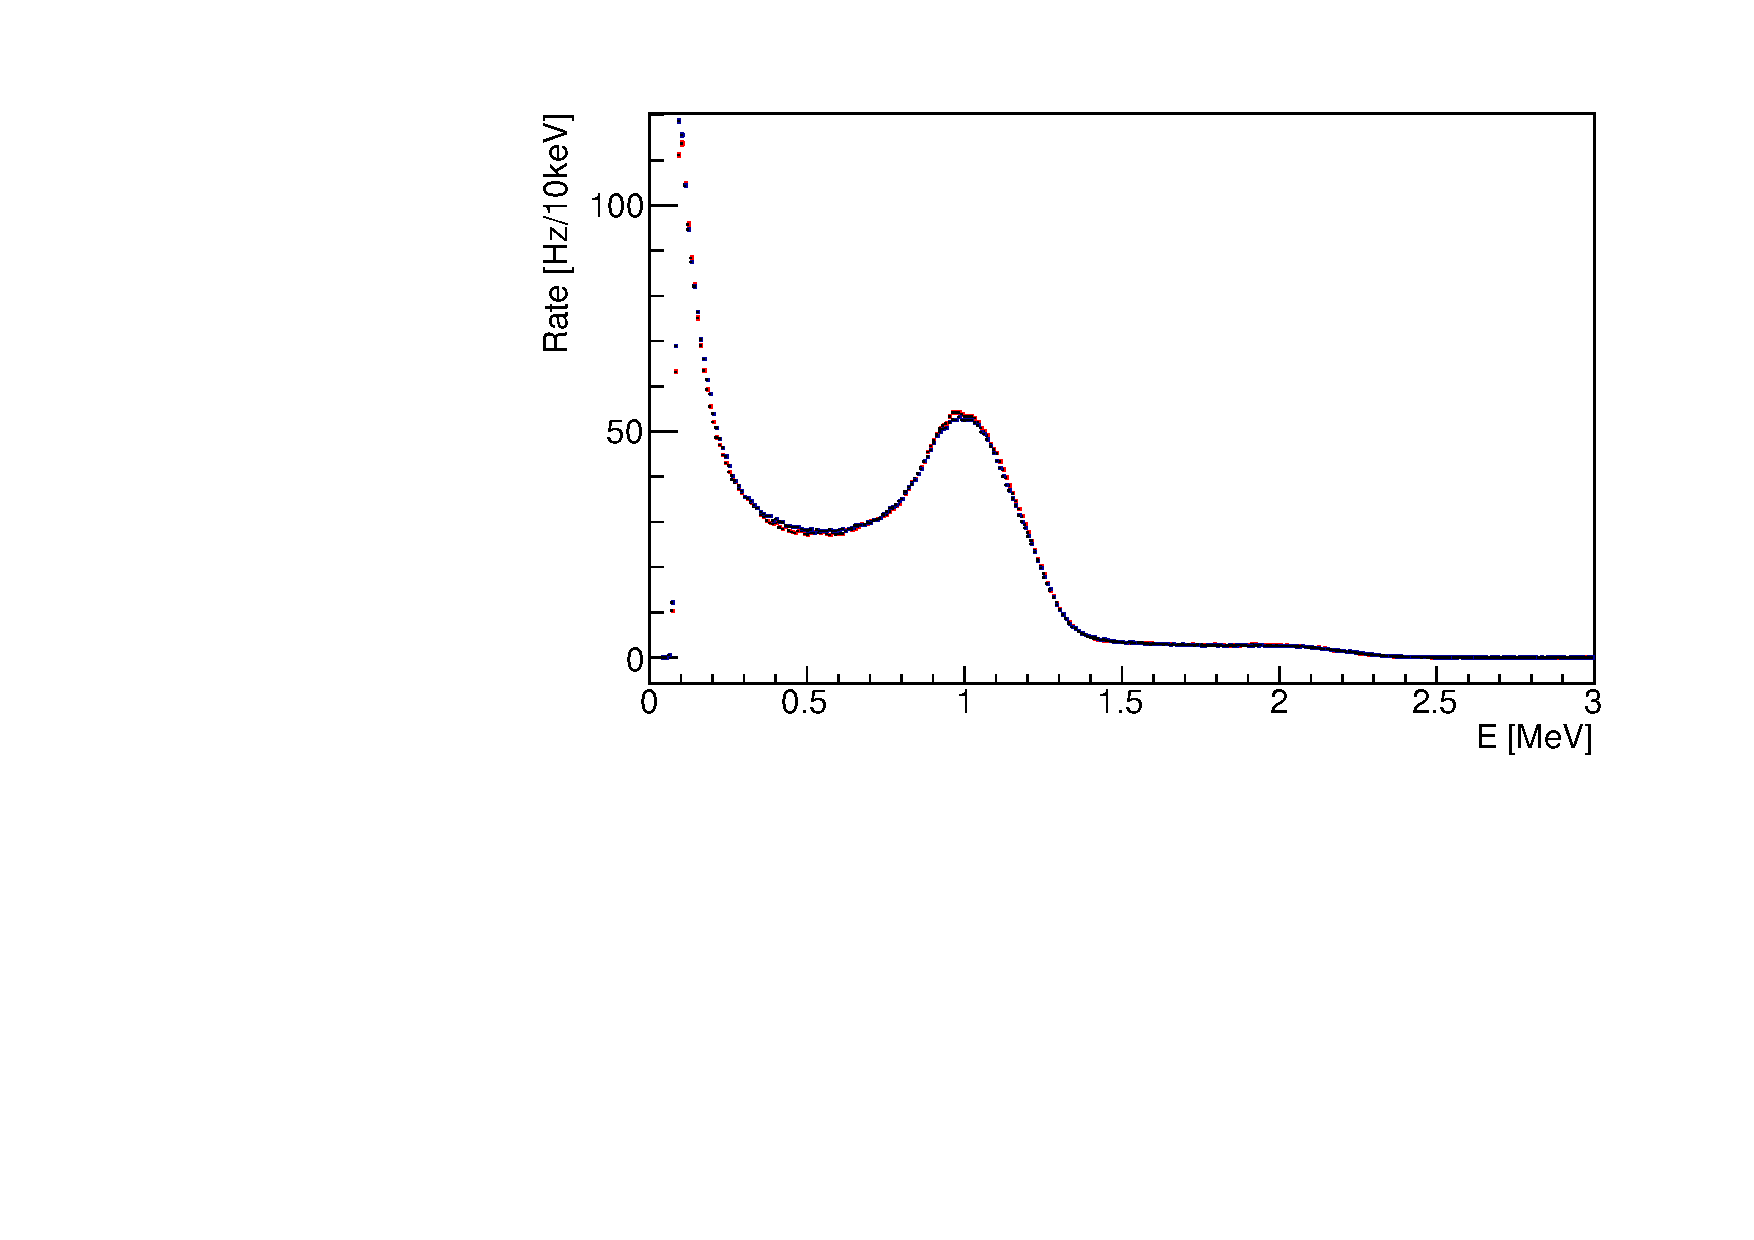
\includegraphics[width=60mm]{figures/hCo60v2single.pdf}} \quad
\subfigure[Best-fit MC-data for n-H gamma.]{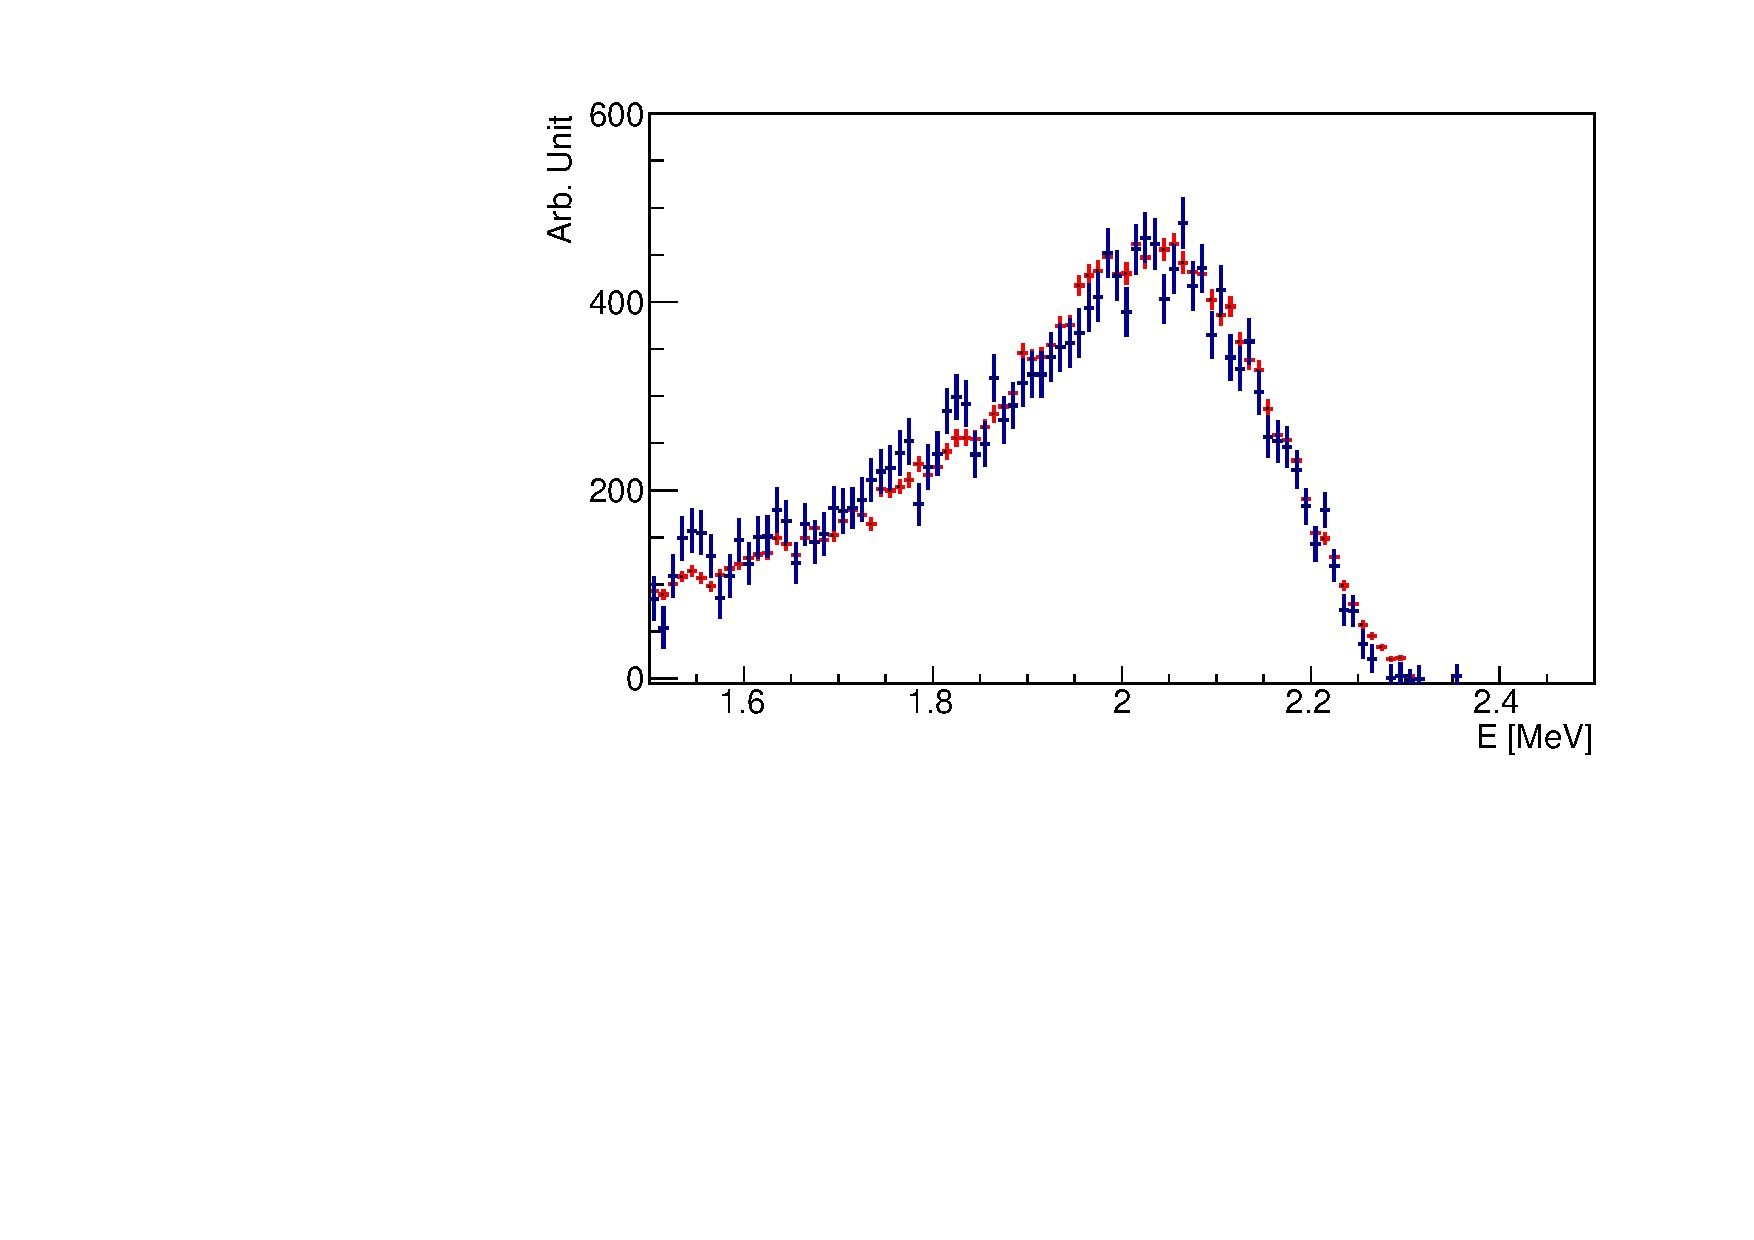
\includegraphics[width=60mm]{figures/hCf252v2single.pdf}} \\
\subfigure[Best-fit MC-data for $^{12}$B]{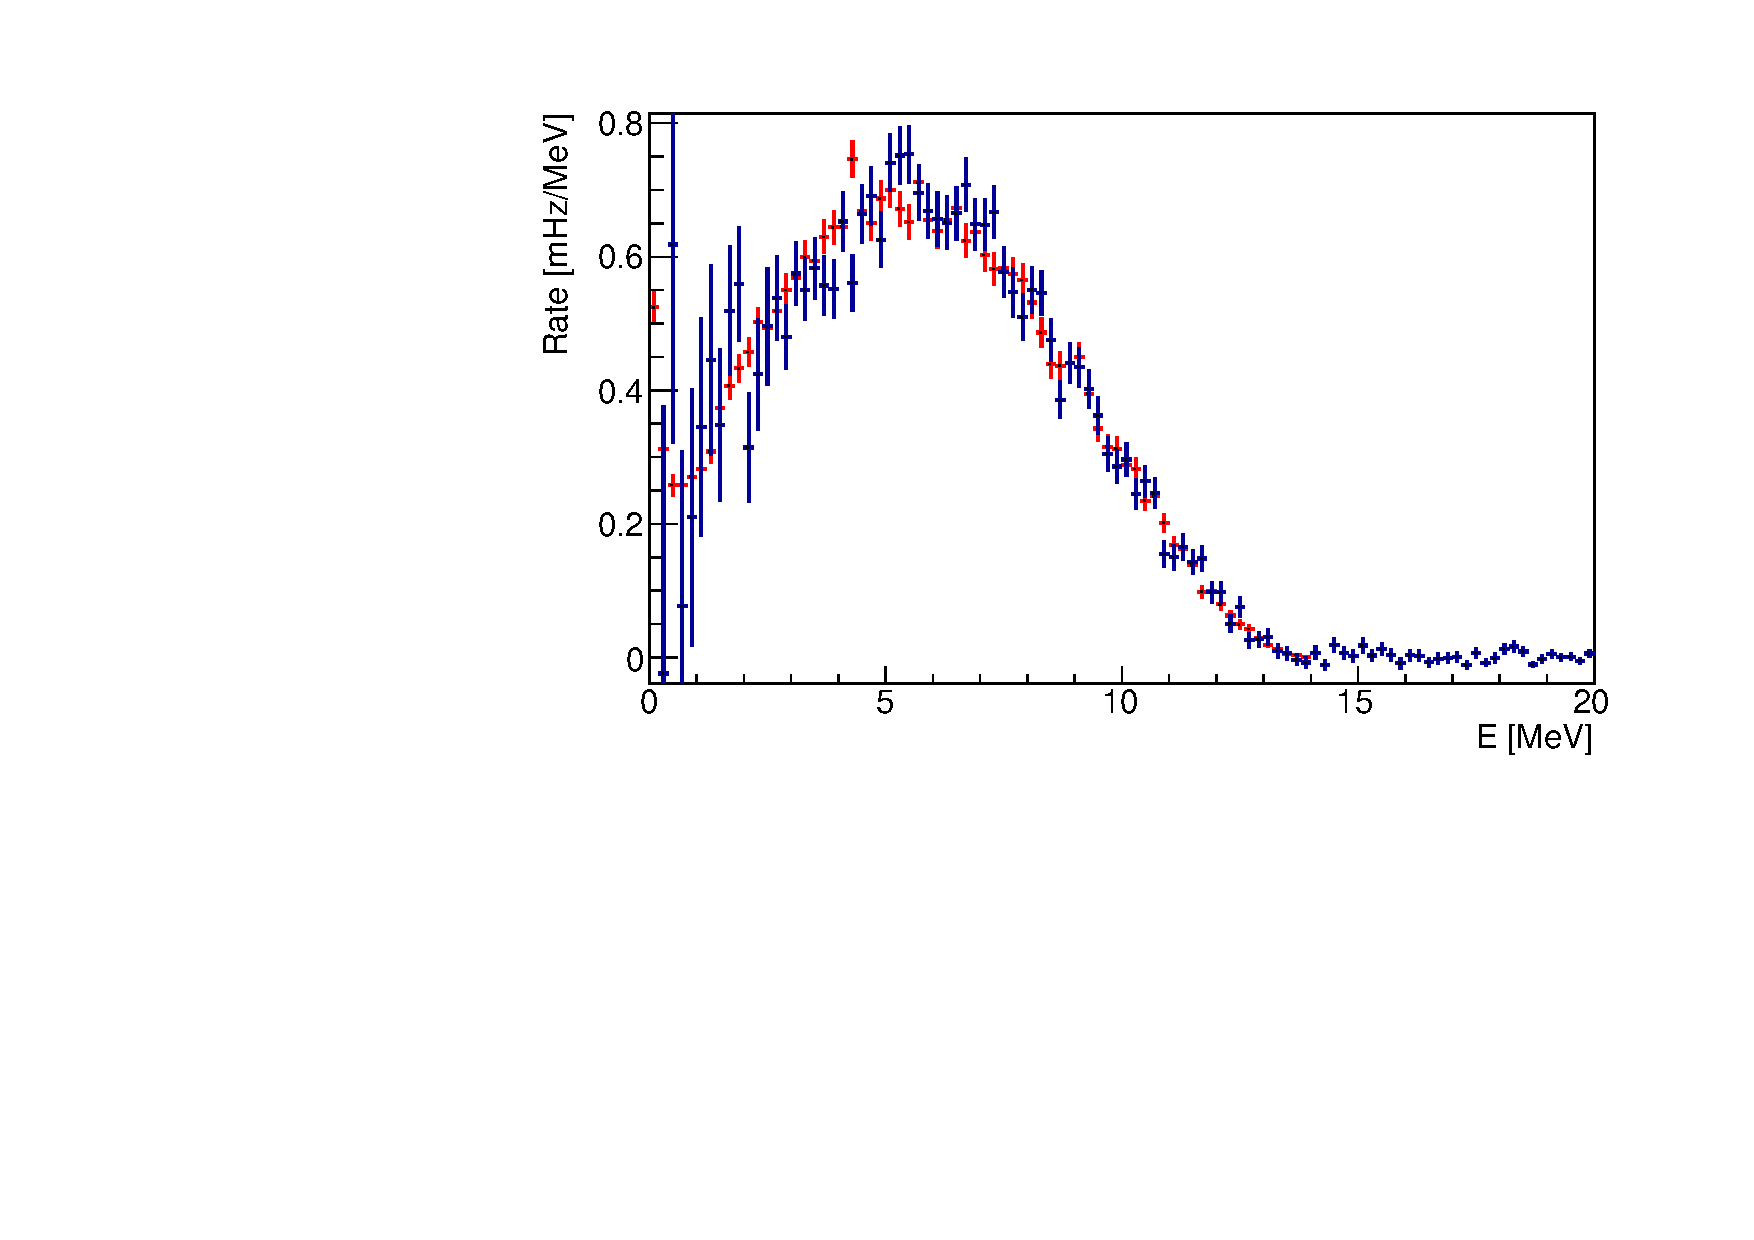
\includegraphics[width=60mm]{figures/hB12v2single.pdf}} 
\caption{The best fit results from single-cell data vs. MC comparison.}
\label{fig:goodfit}
\end{figure}
\newpage
\clearpage

\subsection{Agreement Between Calibration Campaigns}
The energy scale model discussed in previous sections were found with combined fitting of gamma calibrations taken in April 2018, neutron calibration performed in May 2018 and ambient data. 
Idealy, this model ought to be compatible with other calibration campaigns with same configuration. 
Thus we applied the model to the August 2018 calibration, which includes both gamma and neutron calibrations, as a further cross check on the best fit model.
An issue with the August 2018 calibration is that one source was possibly partially left between the detector and shielding volume, shown in Figure \ref{fig:left}.

\begin{figure}[h!]
\centering
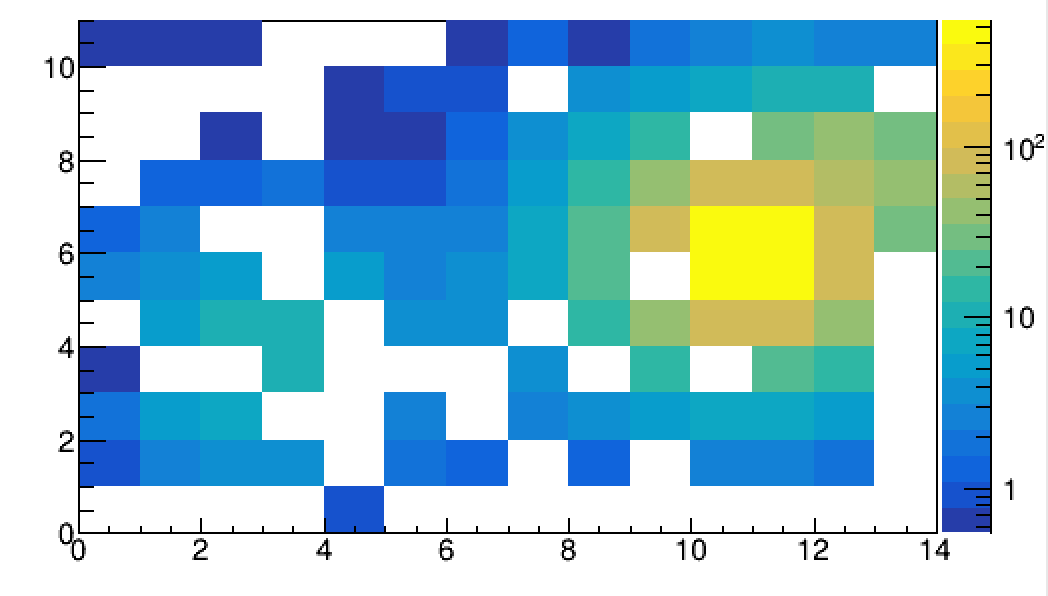
\includegraphics[width=80mm]{figures/secondhotspot.png}
\caption{The event distribution of gamma event cluster, there is a secondary hot spot indicating another source trapped in the volume between detector volume and shielding.}
\label{fig:left}
\end{figure}

To avoid the contamination from the source, instead of measure the full-detector reconstructed energy, the event selection constrained every hits of a cluster being within 3 layers of LS cell from the center, showed in Figure \ref{fig:ring}.
To maintain uniformity in energy spectrum comparison, we applied the 3-layer energy reconstruction on both the April gamma calibration and August gamma calibration, while made neutron calibration and ambient calibration remain-full detector reconstruction because they were not affected by the trapped source.

\begin{figure}[h!]
\centering
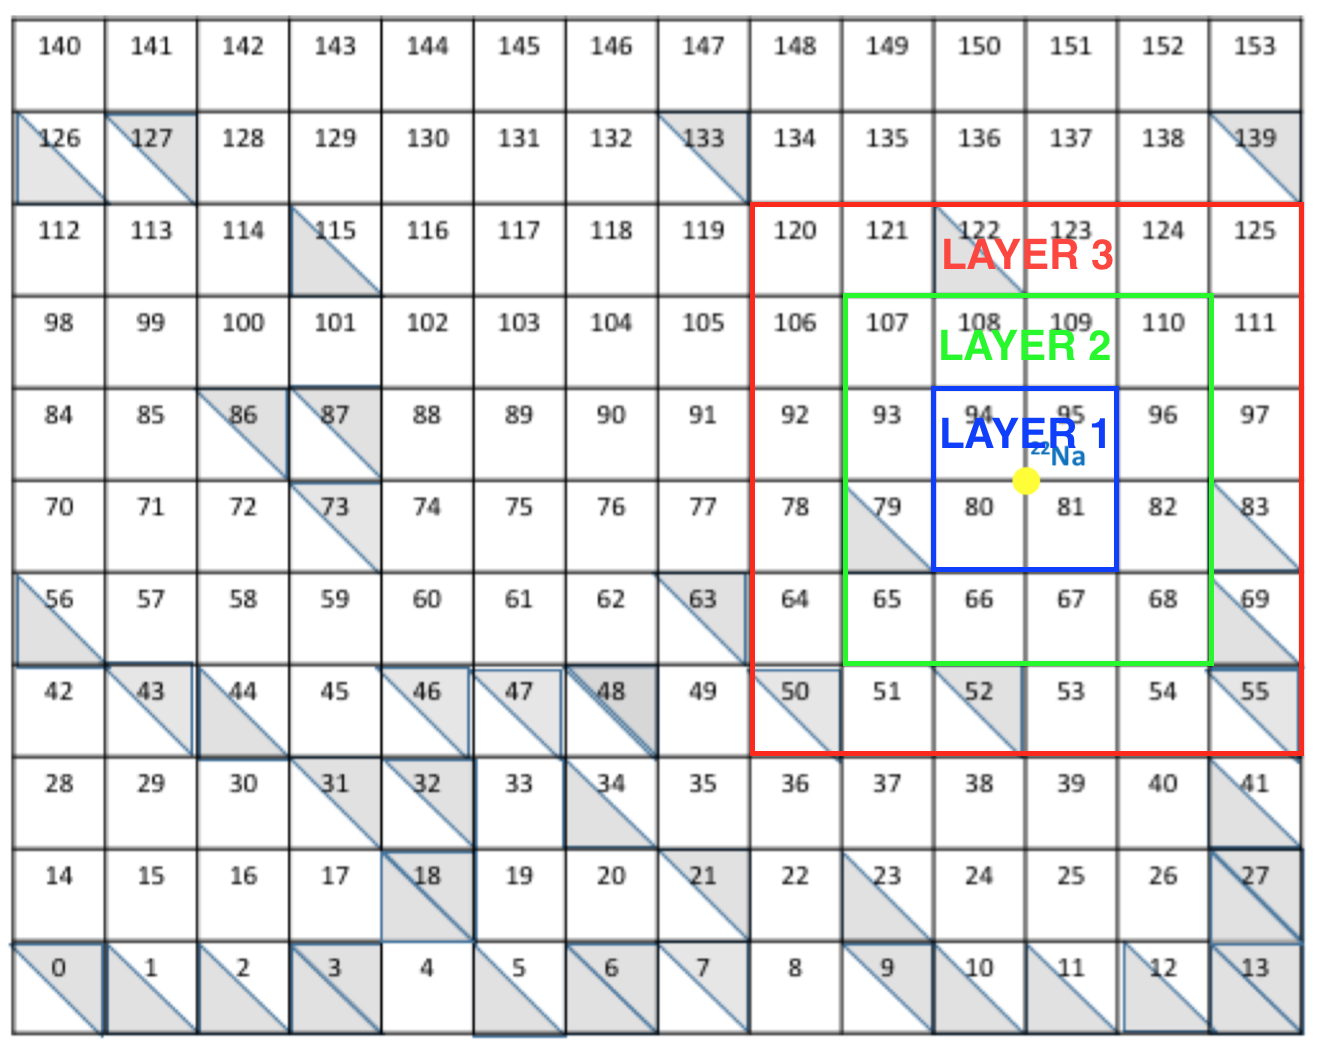
\includegraphics[width=80mm]{figures/Ring.png}
\caption{An example of how 3 layers of LS was defined.}
\label{fig:ring}
\end{figure}

When we reapplied the best-fit nonlinearity model to the April data-MC comparison with 3-layer reconstruction, the total $\chi^2$ value increased from 807.847 to 1082.1, and absolute energy scale shifted from 0.36\% to 0.42\%, indicating unresolved multiplicity disagreement between MC and data.
The $\chi^2/NDF = 2750.78$ when the same model was deployed in August calibration data-MC comparison, with absolute energy scale shift = 0.32
However, as shown in Figure \ref{fig:compare}, the energy scale at discrepancy is within 0.8\% uncertainty.

\begin{figure}[h!]
\centering
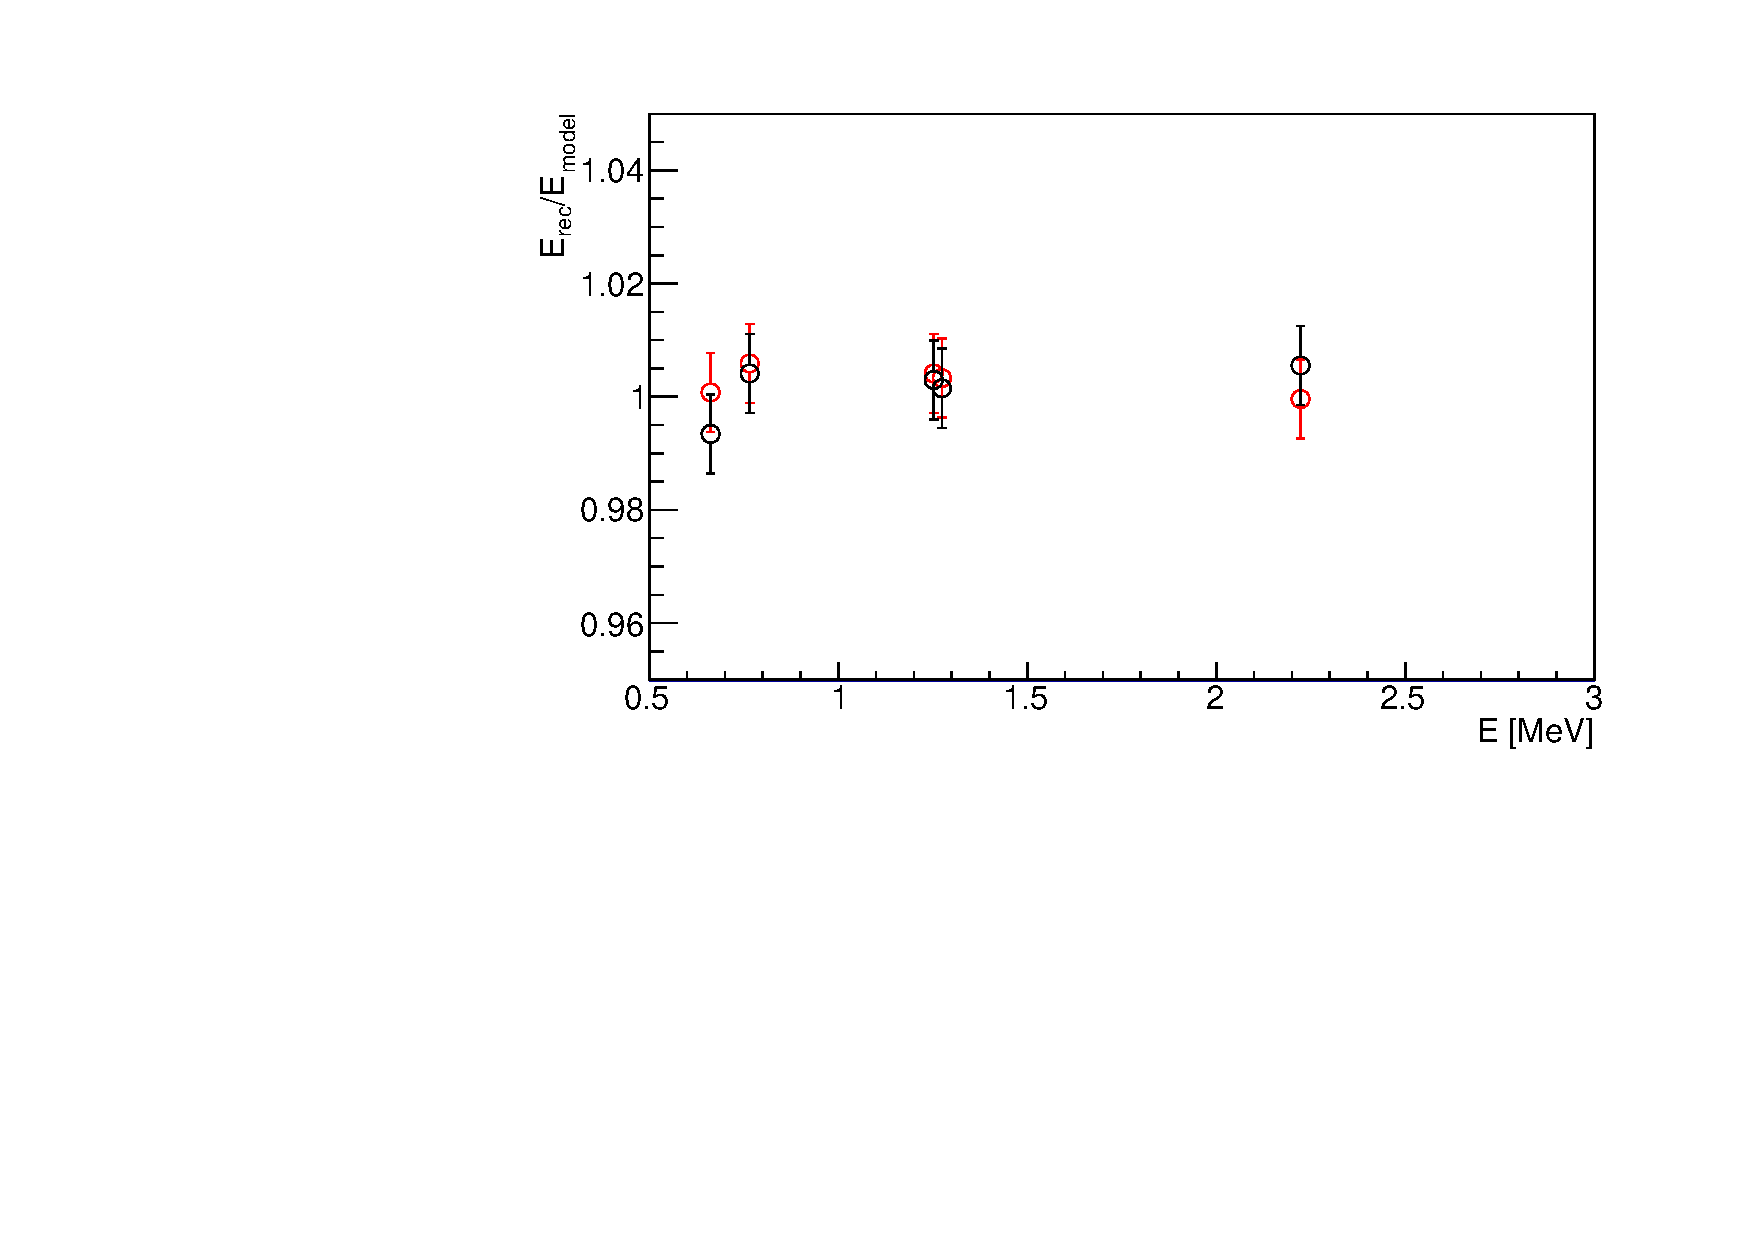
\includegraphics[width=80mm]{figures/EScaleCompare.pdf}
\caption{The discrepancy between April and August calibration energy scale is within $\sim0.8\%$ uncertainty.}
\label{fig:compare}
\end{figure}

\newpage

\section{Final Model and Uncertainties for the Spectrum Analysis}
According to Section \ref{sec:dataMC}, we finalized the energy nonlinearity model based on the single-cell data vs. MC comparison.
The energy scale of PROSPECT AD can be expressed as the ratio of true energy to reconstructed energy of average particle from different calibrations $E_{rec}/E_{true}$ as shown in Figure \ref{fig:escale}, which indicates at lower energy, the scale is able to vary $\sim0.8\%$ from 100\%, where 0.2\% came from energy scale fluctuation caused by nonlinearity model uncertainty, the 0.6\% will be discussed in the next paragraph.

\begin{figure}[h!]
\centering
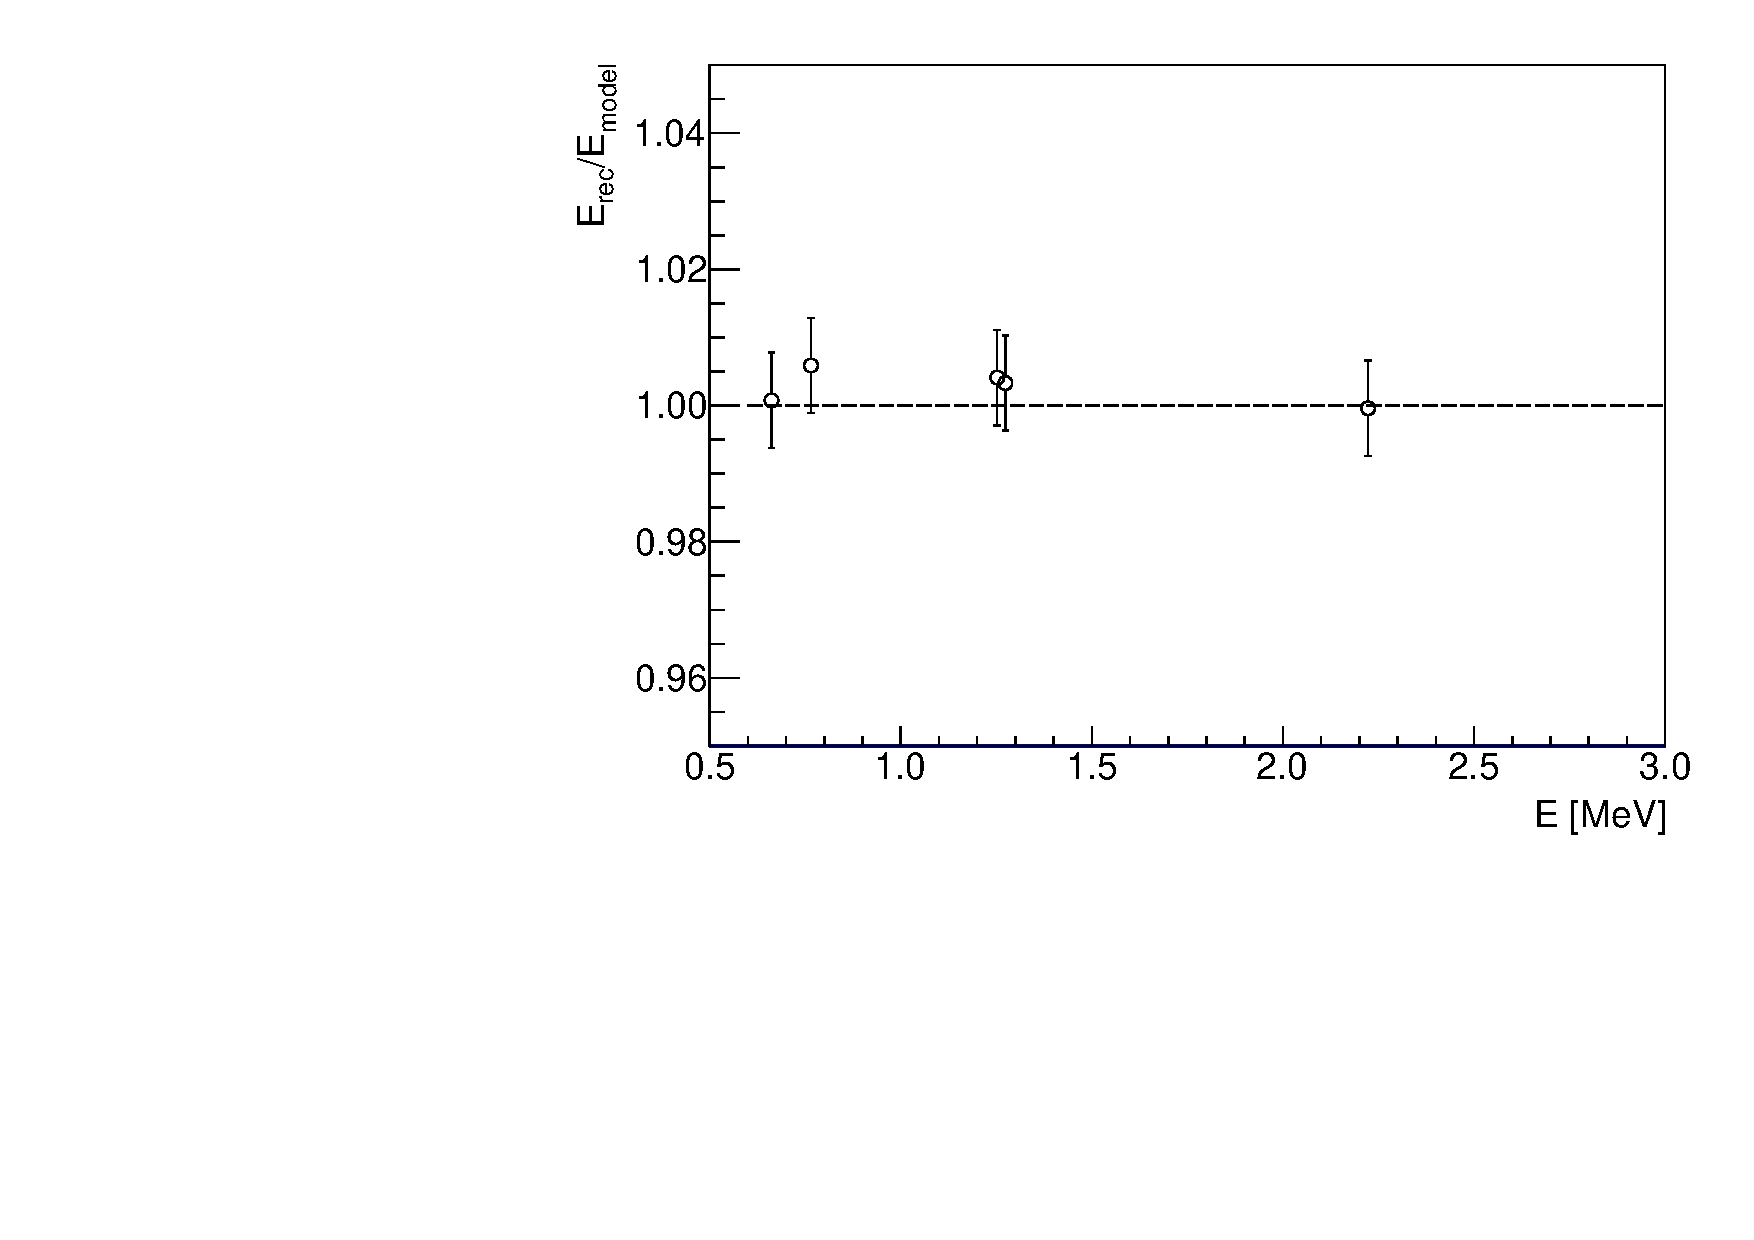
\includegraphics[width=80mm]{figures/EScale.pdf}
\caption{The reconstructed energy to true energy ratio.}
\label{fig:escale}
\end{figure}

The $^{12}$B energy spectrum data vs MC comparison was used to demonstrate the energy scale at higher energy, shown in Figure \ref{fig:B12final}. 

\begin{figure}[h!]
\centering
\subfigure[Full detector MC-data comparison for $^{12}$B spectrum.]{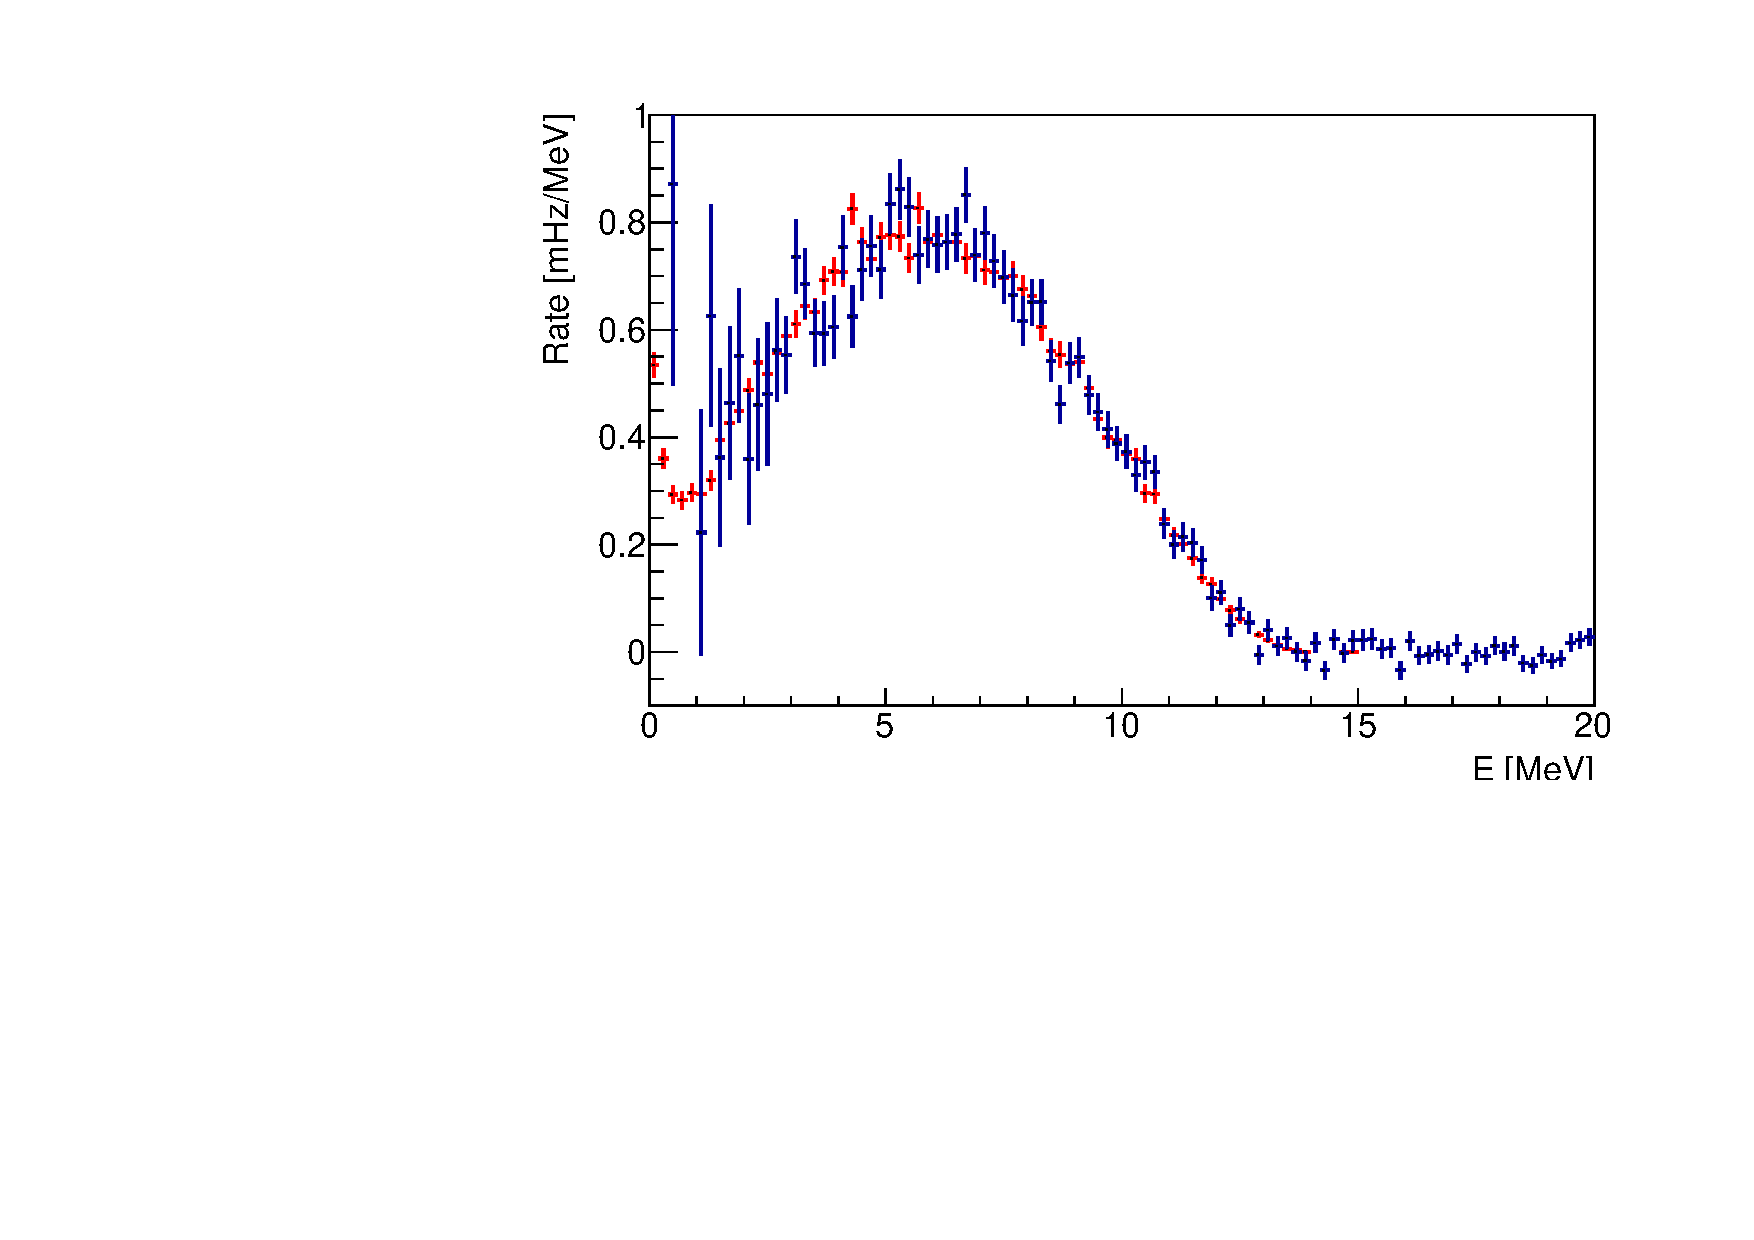
\includegraphics[width=60mm]{figures/hB12v2.pdf}} \quad
\subfigure[The residual of this comparison.]{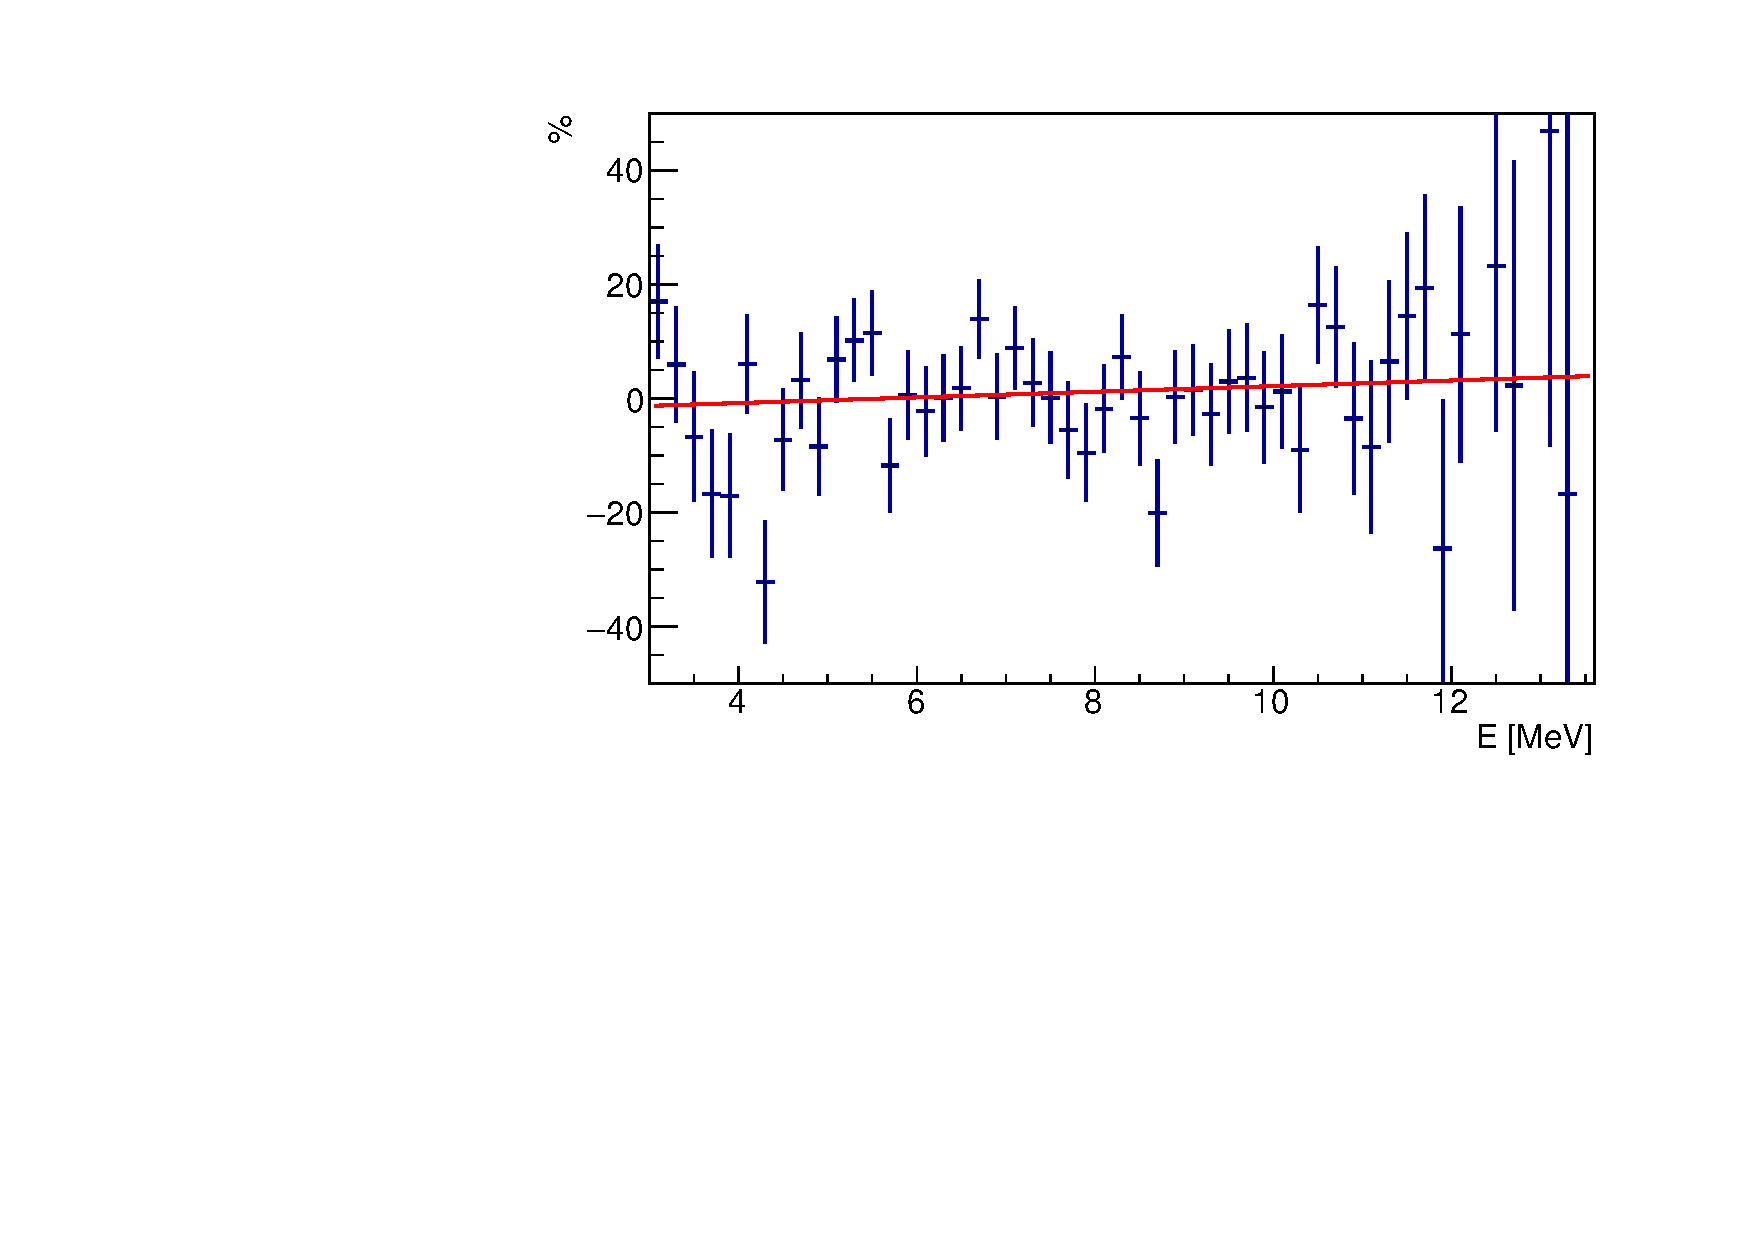
\includegraphics[width=60mm]{figures/hB12residualv2.pdf}} \quad
\caption{The average residual of this comparison found the to be $0.49 \pm 0.60\%$}
\label{fig:B12final}
\end{figure}

The energy resolution in Figure \ref{fig:resolution} shows the resolution of each energy distributions of calibrations, fitted with Function \ref{eql:resolution}.

\begin{figure}[h!]
\centering
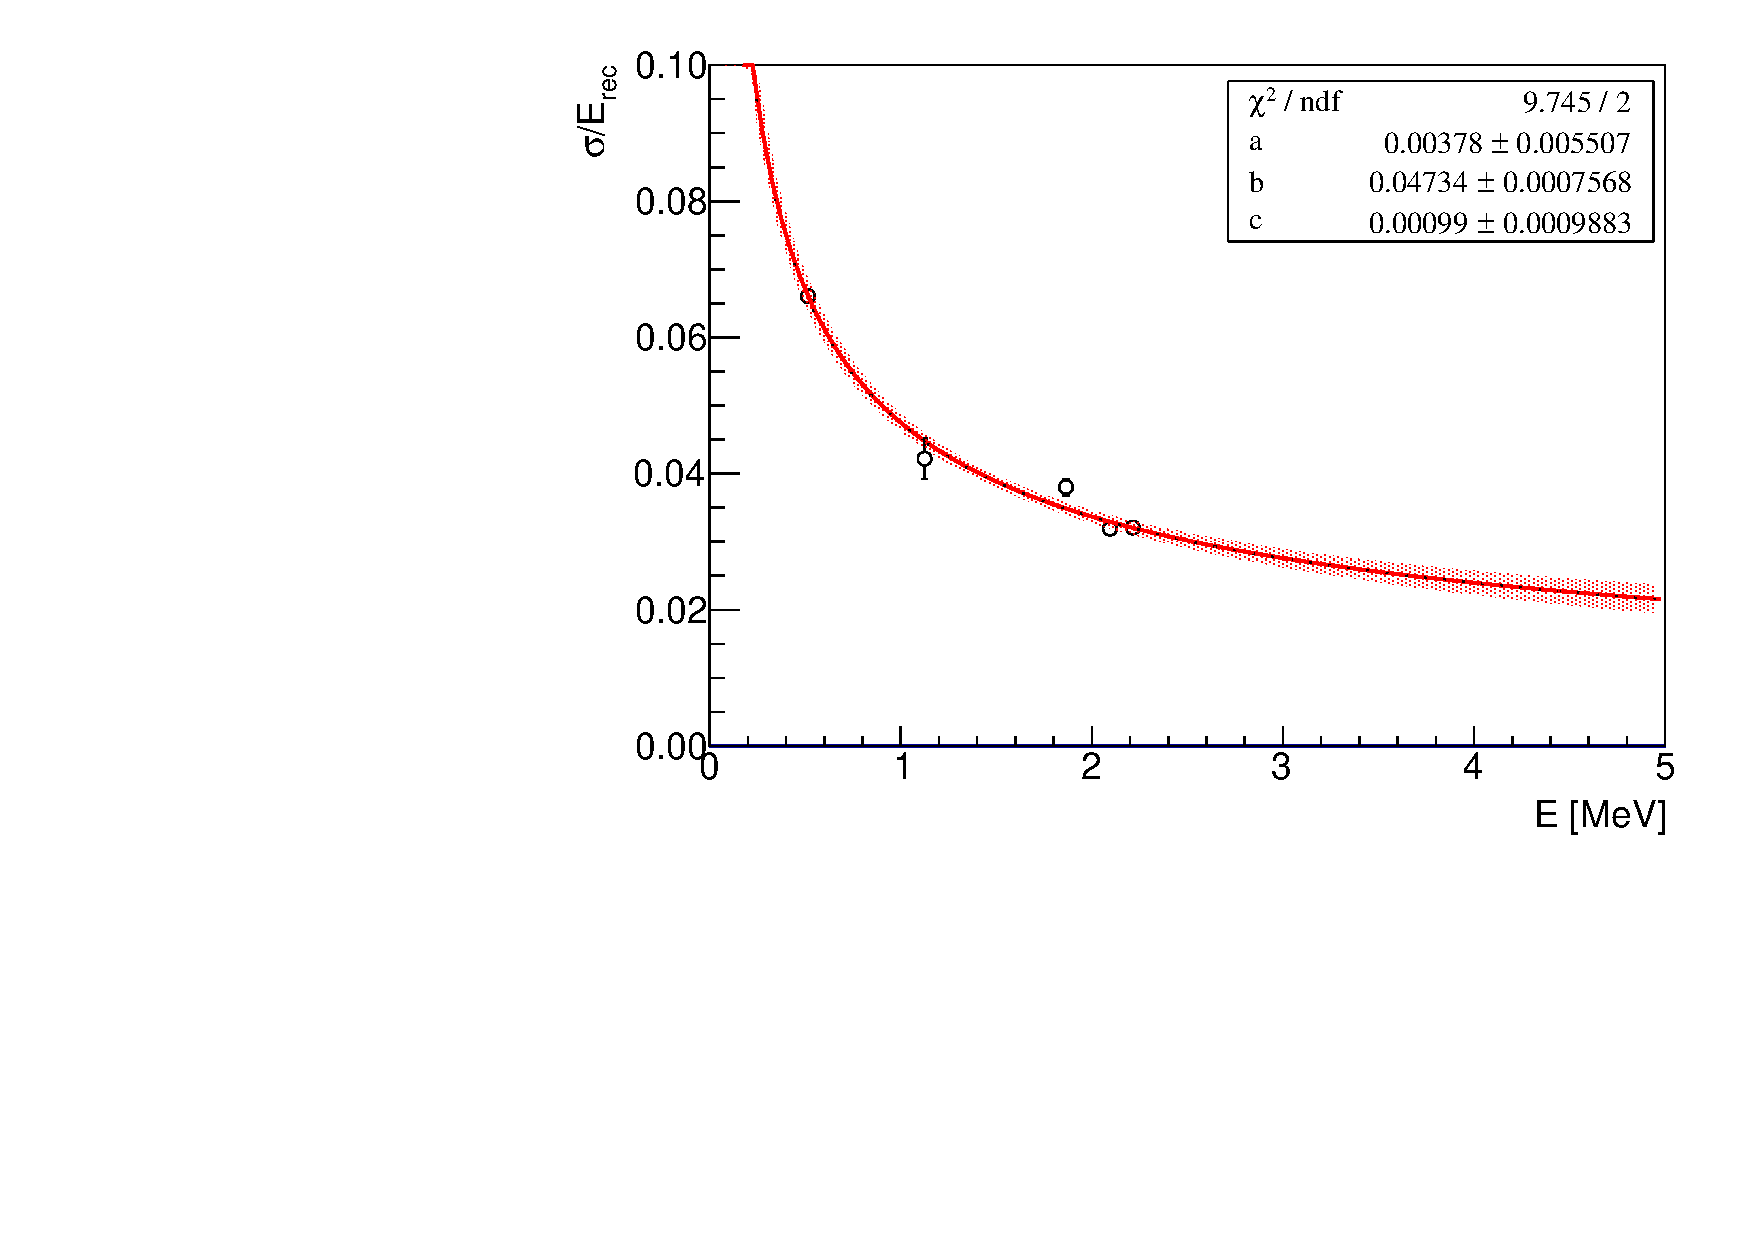
\includegraphics[width=80mm]{figures/Resolution.pdf}
\caption{The energy resolution of mean energies of each calibration fitted with resolution function. (errors are currently statisical only)}
\label{fig:resolution}
\end{figure}

The data vs. MC comparison of $^{22}$Na gamma spectrum is a good way to indicate the multi-particle event reconstructino of PROSPECT AD, see Figure \ref{fig:Na22final}.

\begin{figure}[h!]
\centering
\subfigure[Full detector data-MC comparison for $^{22}$Na calibration.]{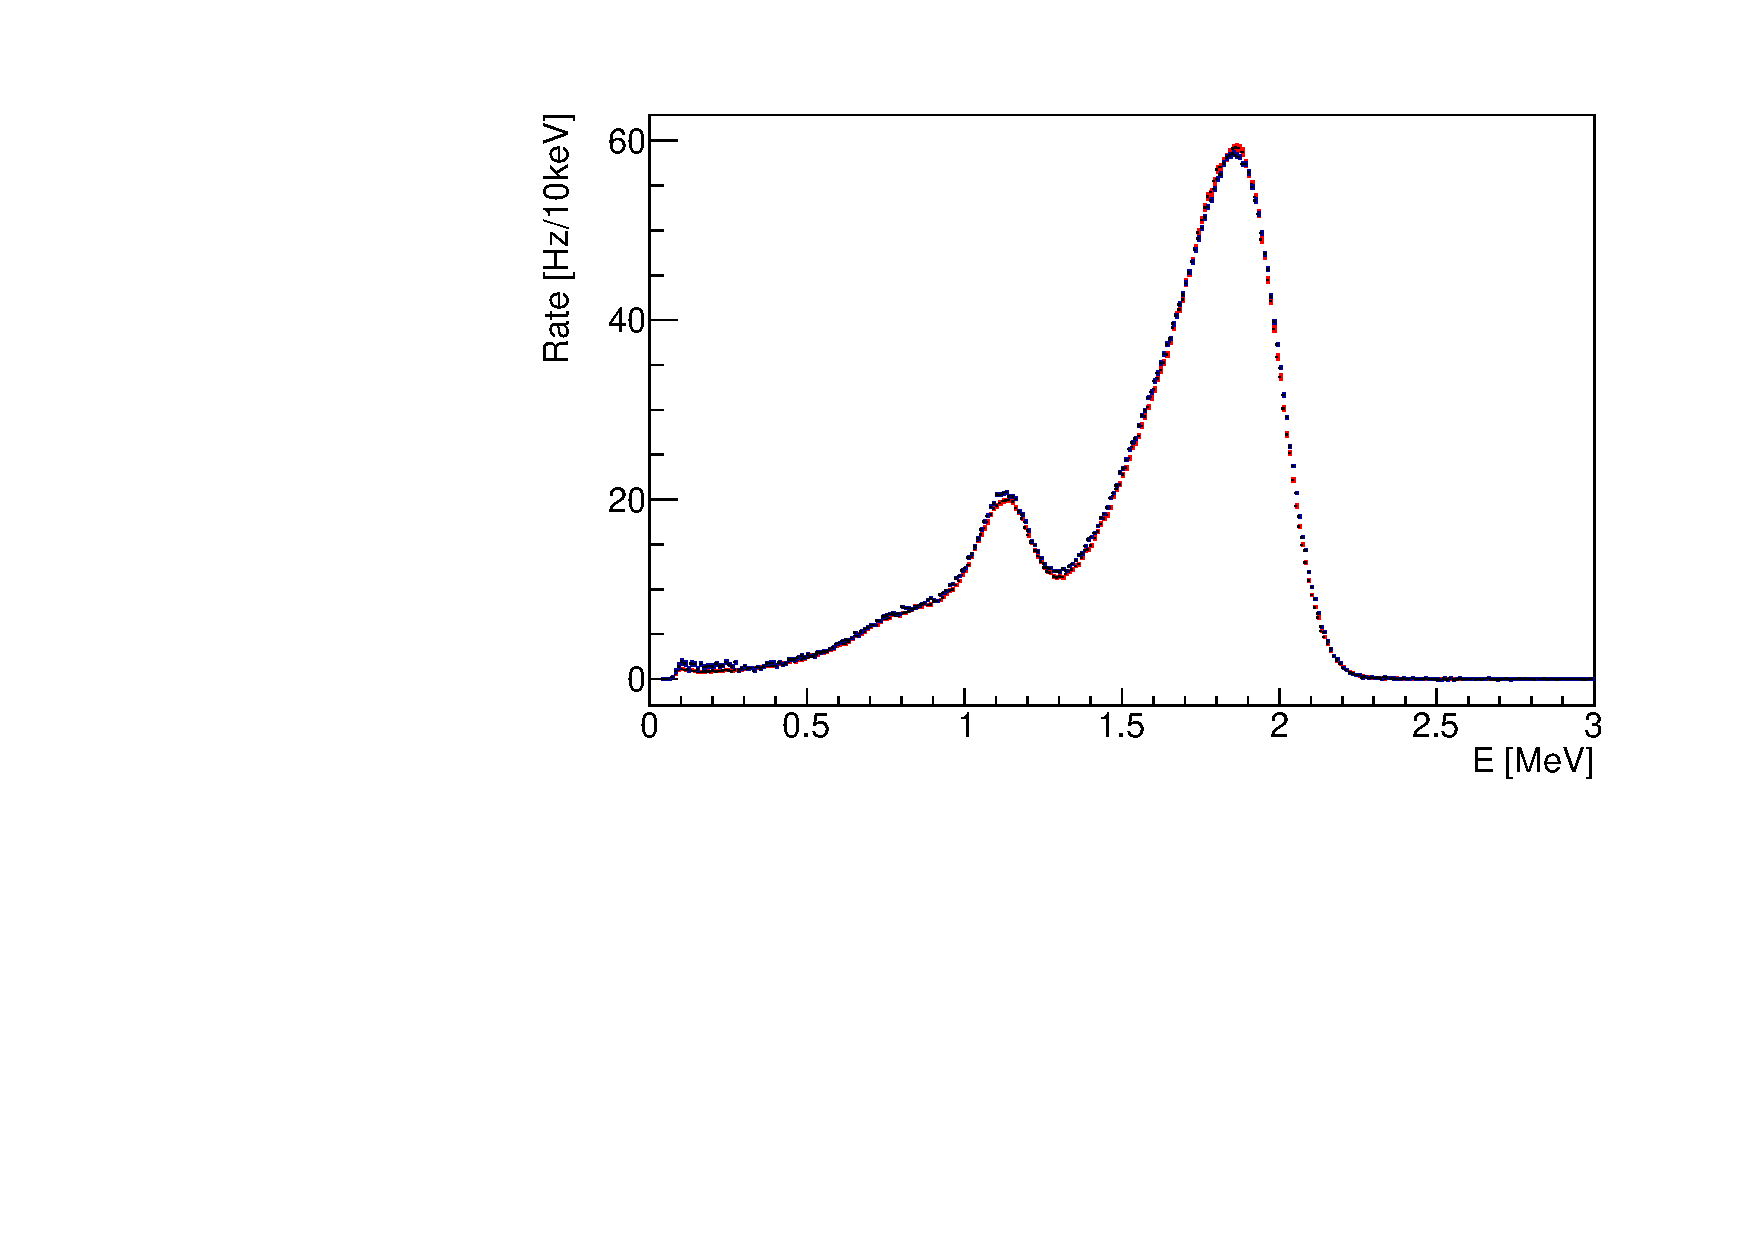
\includegraphics[width=60mm]{figures/hNa22v2.pdf}} \quad
\subfigure[The residual of this comparison.]{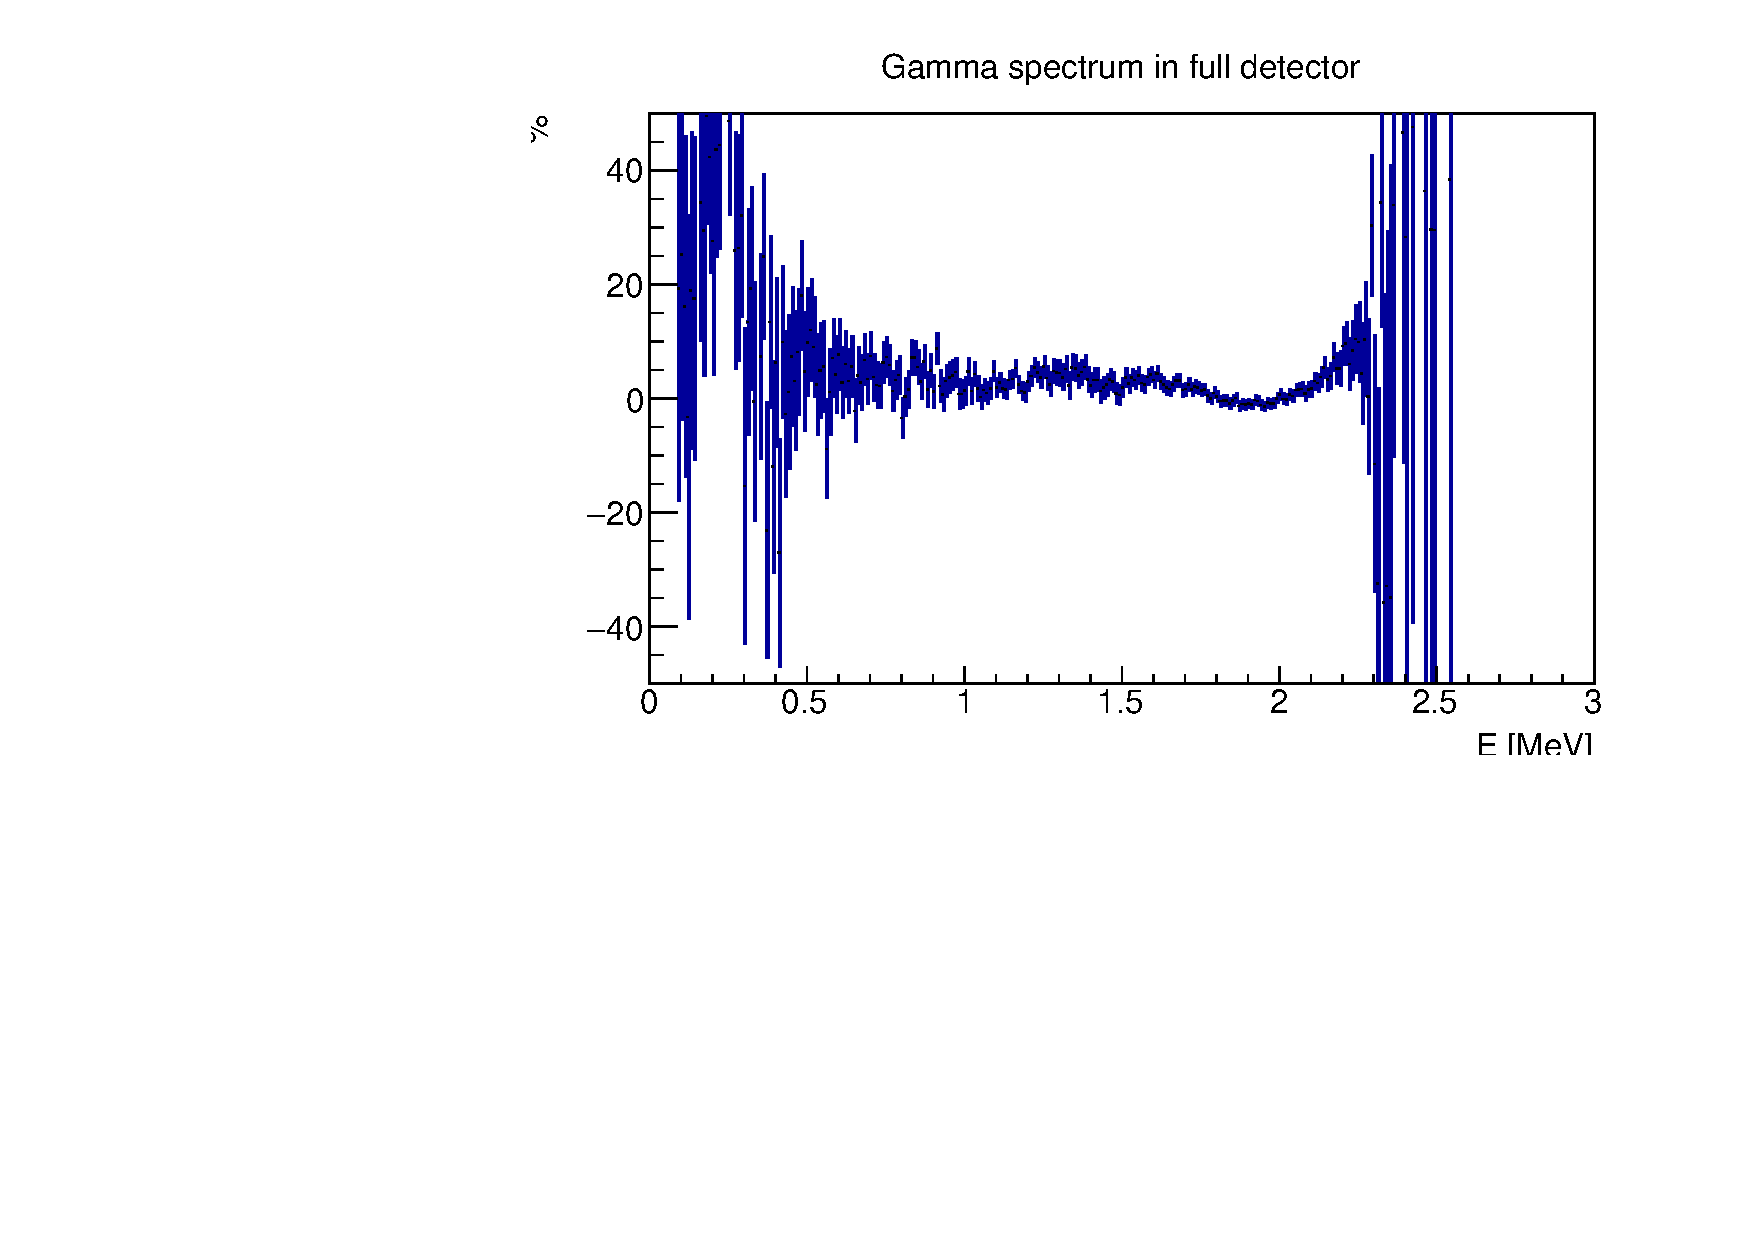
\includegraphics[width=60mm]{figures/hNa22residual.pdf}} \quad
\caption{The data-MC comparison of $^{22}$Na spectrum and residual of comparison.}
\label{fig:Na22final}
\end{figure}

\newpage
The gamma calibration sources supplied sufficient amount of statistics. 
The $0.60\%$ energy scale uncertainty and statistical uncertainty of $^{12}$B spectrum smeared the $\chi^2$ distribution during the quenching model search, thus enlarged uncertainty of nonlinearity model. 
We chose to be conservative and treat the 0.6\% energy scale uncertainty in $^{12}$B as an systematic energy scale uncertainty.
The energy resolution in spectrum analysis are forced to be smeared with respect to the poorest resolution measured in detector during data taking.

In conclusion, the uncertainty of energy response is dominated by the systematic uncertainties:

\begin{itemize}
    \item The $1-\sigma$ uncertainty of Birks$^\prime$ constants and Cherenkov efficiency.
    \item The 0.6\% uncertainty of absolute energy scale.
    \item The thresholding uncertainty of $85\pm5$ keV.
    \item The uncertainty of the artificial smearing $400\pm8$ PE/MeV.
    \item The uncertainty of thickness of separator of $1.18\pm0.05$ mm.
\end{itemize}
Each of the uncertainties above are turned into covariance matrix individually. 
As a result, the covariance matrices of energy scale uncertainty and thickness of separator are shonwn in Figure \ref{fig:cov}.

\begin{figure}[h!]
\centering
\subfigure[Covariance matrix for the uncertainty in nonlinearity and energy scale model.]{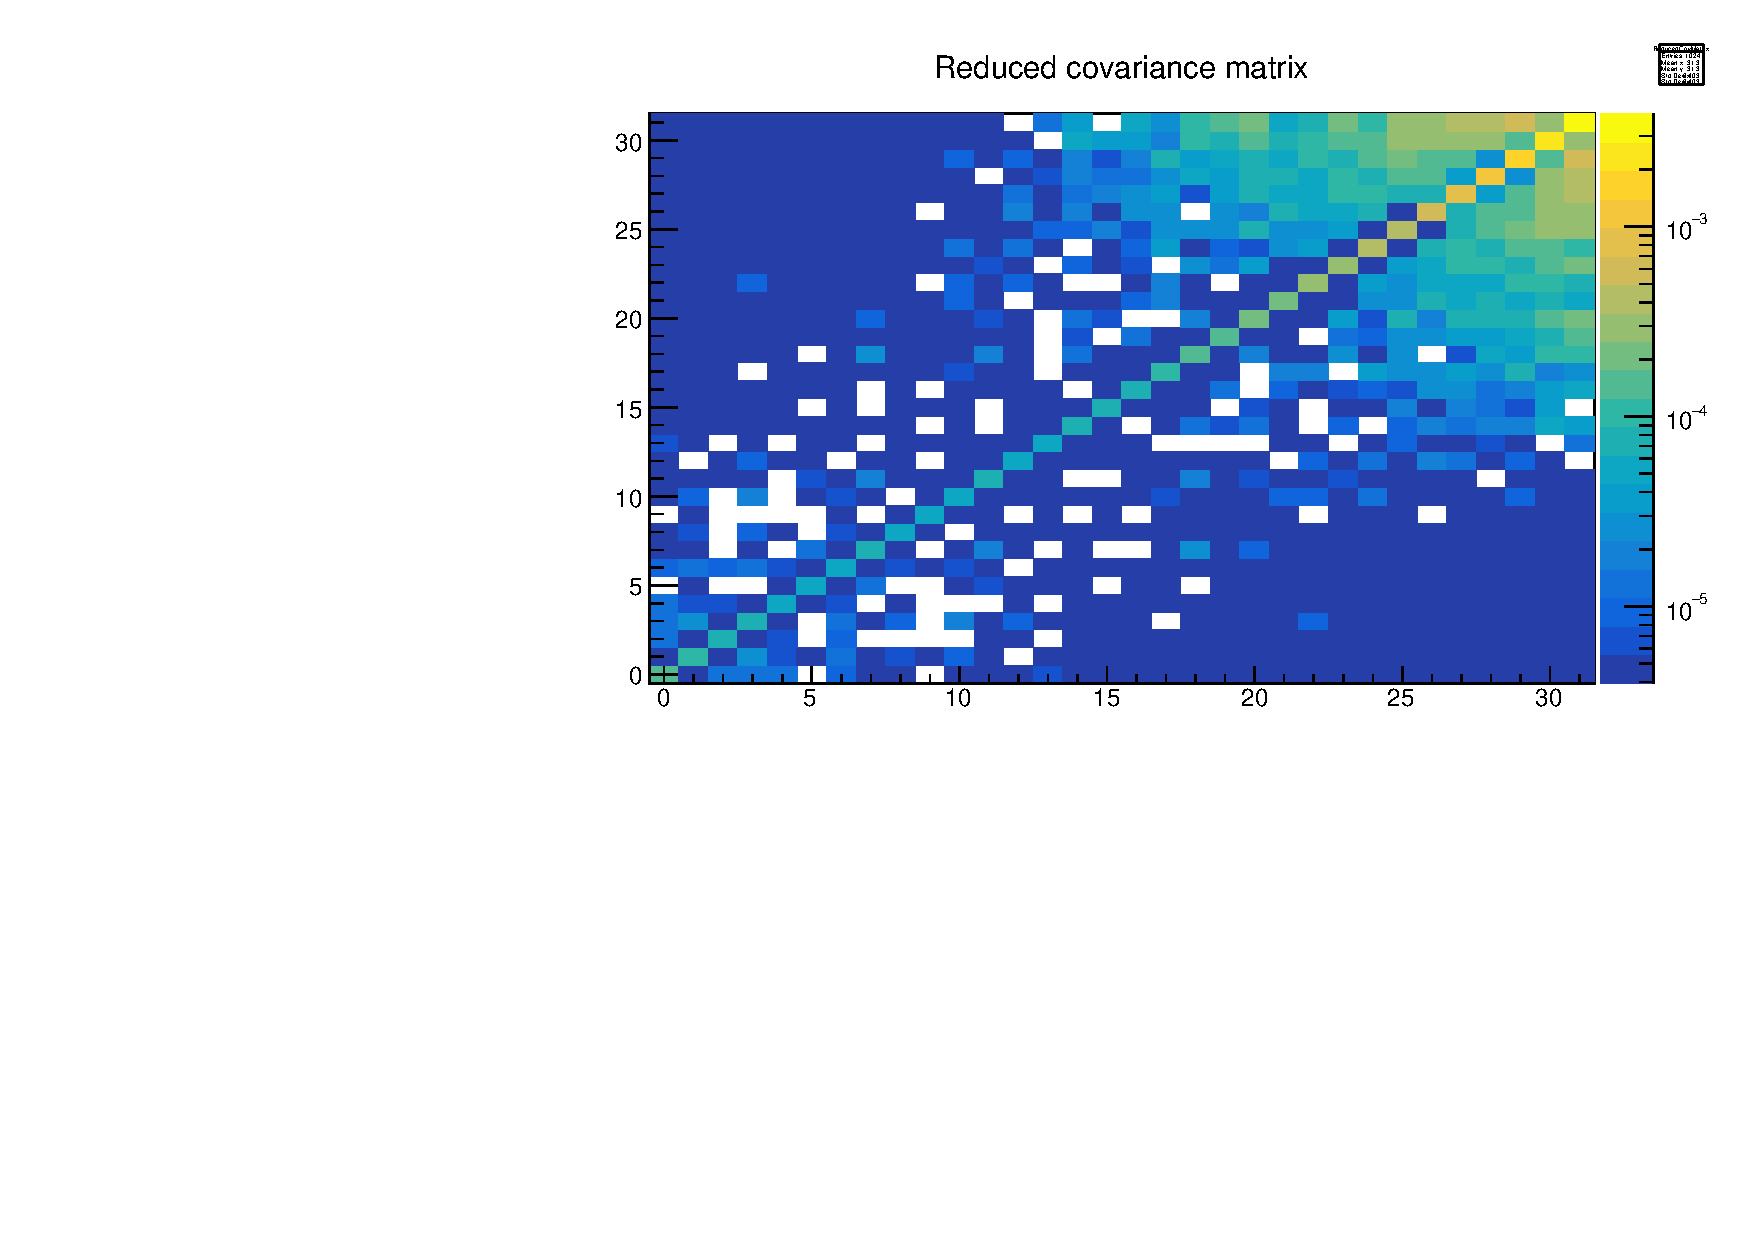
\includegraphics[width=60mm]{figures/nonlinearcov.pdf}} \quad
\subfigure[Covariance matrix for the uncertainty of panel thickness.]{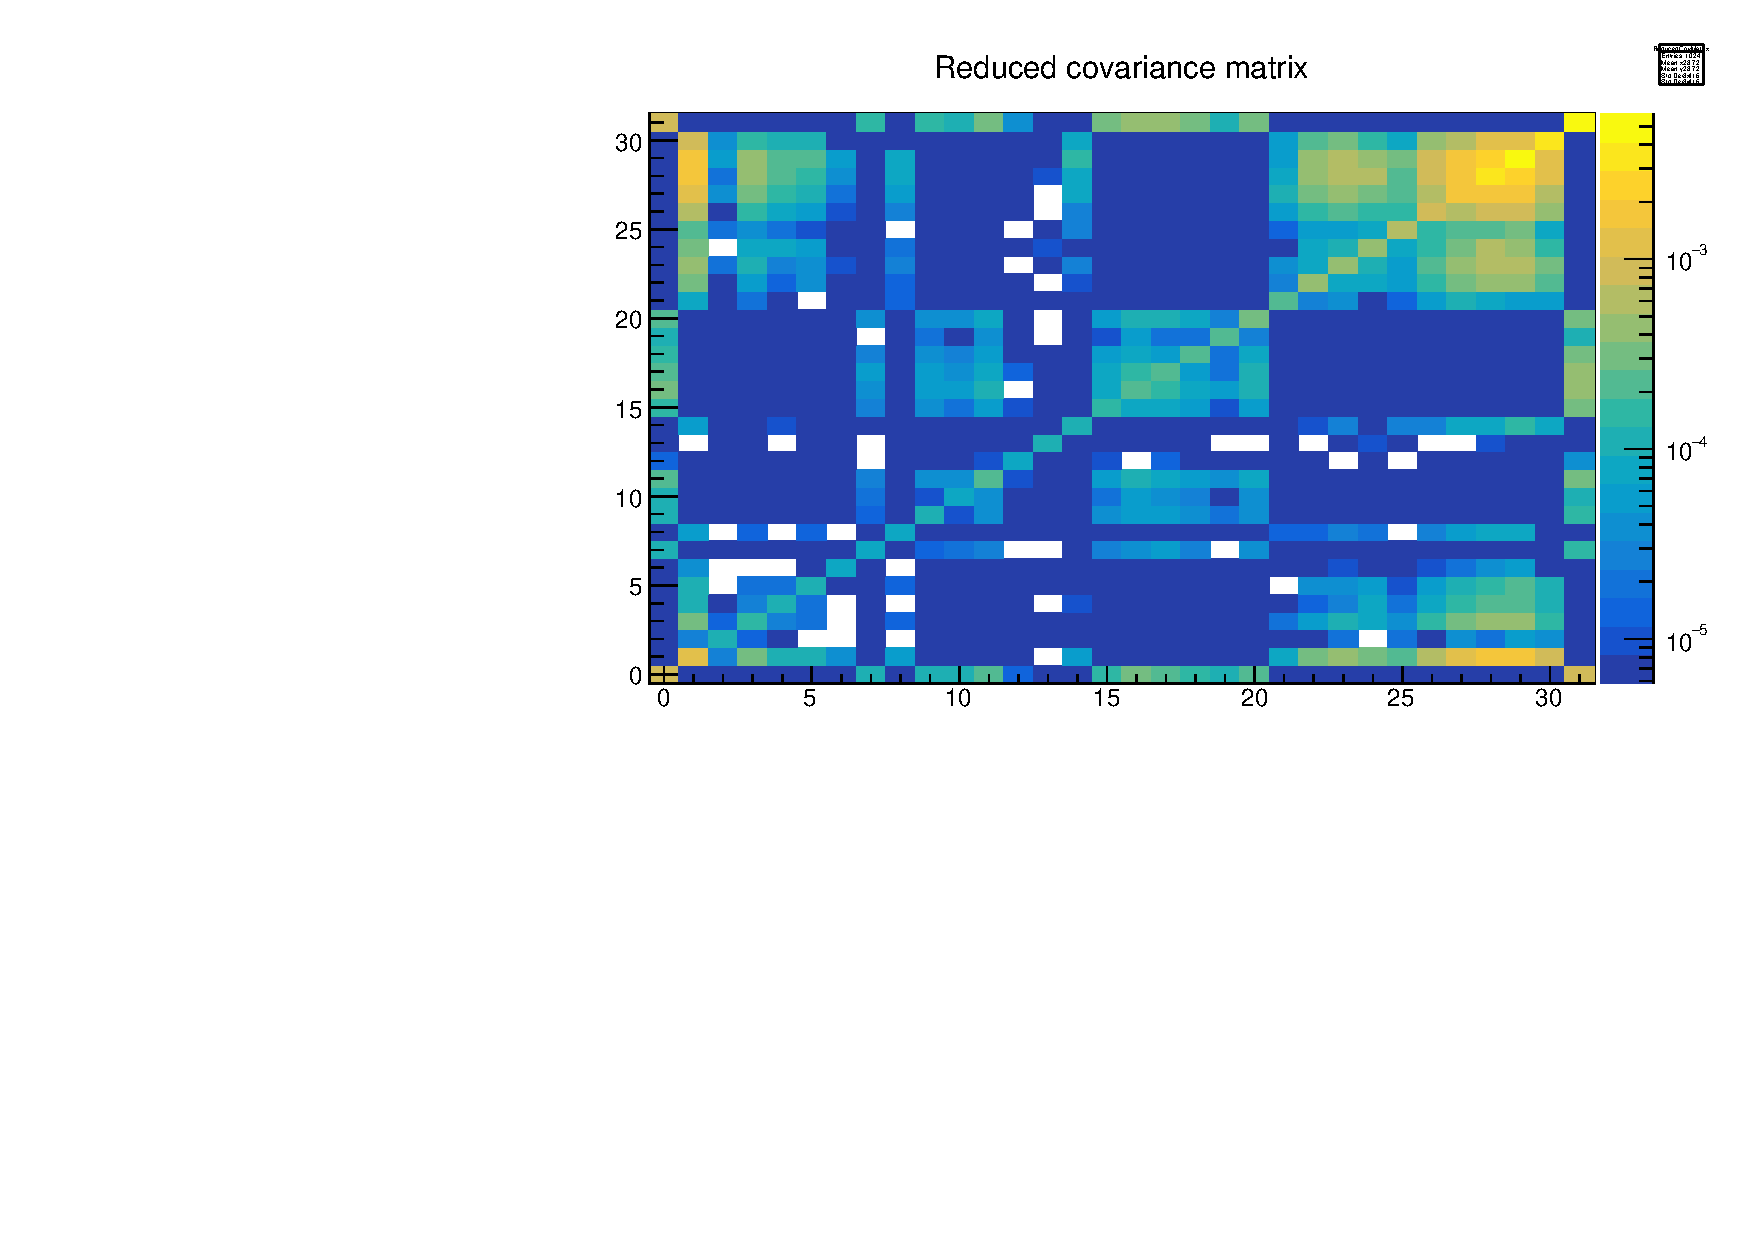
\includegraphics[width=60mm]{figures/thickcov.pdf}} \quad
\caption{Current reduced covariance matrices.}
\label{fig:cov}
\end{figure}

\section{Conclusion}

We are able to finalize the dominant parameters in energy scale study, which are $k_{B1} = 0.122 \pm 0.002$ mm/MeV, $k_{B2} = 0.032 \pm 0.002$ mm/MeV, $k_C = 41 \pm 1\%$, $\beta_{rec} = 100.36\pm0.6\%$.
The uncertainties in energy scale is mainly the uncertainty of parameters and separator thickness.
There are unresolved disagreement between full-detector best fit and single-cell best fit as well as multiplicity discrepancy that hinted further adjustments on detector geometry or material property.


%\newpage
%\appendix
%\section{...}
%\label{sec:resources}

%TODO edit bibliography
\newpage
\bibliography{citations.bib}{}

\end{document}